\documentclass[twoside]{book}

% Packages required by doxygen
\usepackage{fixltx2e}
\usepackage{calc}
\usepackage{doxygen}
\usepackage[export]{adjustbox} % also loads graphicx
\usepackage{graphicx}
\usepackage[utf8]{inputenc}
\usepackage{makeidx}
\usepackage{multicol}
\usepackage{multirow}
\PassOptionsToPackage{warn}{textcomp}
\usepackage{textcomp}
\usepackage[nointegrals]{wasysym}
\usepackage[table]{xcolor}

% Font selection
\usepackage[T1]{fontenc}
\usepackage[scaled=.90]{helvet}
\usepackage{courier}
\usepackage{amssymb}
\usepackage{sectsty}
\renewcommand{\familydefault}{\sfdefault}
\allsectionsfont{%
  \fontseries{bc}\selectfont%
  \color{darkgray}%
}
\renewcommand{\DoxyLabelFont}{%
  \fontseries{bc}\selectfont%
  \color{darkgray}%
}
\newcommand{\+}{\discretionary{\mbox{\scriptsize$\hookleftarrow$}}{}{}}

% Page & text layout
\usepackage{geometry}
\geometry{%
  a4paper,%
  top=2.5cm,%
  bottom=2.5cm,%
  left=2.5cm,%
  right=2.5cm%
}
\tolerance=750
\hfuzz=15pt
\hbadness=750
\setlength{\emergencystretch}{15pt}
\setlength{\parindent}{0cm}
\setlength{\parskip}{3ex plus 2ex minus 2ex}
\makeatletter
\renewcommand{\paragraph}{%
  \@startsection{paragraph}{4}{0ex}{-1.0ex}{1.0ex}{%
    \normalfont\normalsize\bfseries\SS@parafont%
  }%
}
\renewcommand{\subparagraph}{%
  \@startsection{subparagraph}{5}{0ex}{-1.0ex}{1.0ex}{%
    \normalfont\normalsize\bfseries\SS@subparafont%
  }%
}
\makeatother

% Headers & footers
\usepackage{fancyhdr}
\pagestyle{fancyplain}
\fancyhead[LE]{\fancyplain{}{\bfseries\thepage}}
\fancyhead[CE]{\fancyplain{}{}}
\fancyhead[RE]{\fancyplain{}{\bfseries\leftmark}}
\fancyhead[LO]{\fancyplain{}{\bfseries\rightmark}}
\fancyhead[CO]{\fancyplain{}{}}
\fancyhead[RO]{\fancyplain{}{\bfseries\thepage}}
\fancyfoot[LE]{\fancyplain{}{}}
\fancyfoot[CE]{\fancyplain{}{}}
\fancyfoot[RE]{\fancyplain{}{\bfseries\scriptsize Generated by Doxygen }}
\fancyfoot[LO]{\fancyplain{}{\bfseries\scriptsize Generated by Doxygen }}
\fancyfoot[CO]{\fancyplain{}{}}
\fancyfoot[RO]{\fancyplain{}{}}
\renewcommand{\footrulewidth}{0.4pt}
\renewcommand{\chaptermark}[1]{%
  \markboth{#1}{}%
}
\renewcommand{\sectionmark}[1]{%
  \markright{\thesection\ #1}%
}

% Indices & bibliography
\usepackage{natbib}
\usepackage[titles]{tocloft}
\setcounter{tocdepth}{3}
\setcounter{secnumdepth}{5}
\makeindex

% Hyperlinks (required, but should be loaded last)
\usepackage{ifpdf}
\ifpdf
  \usepackage[pdftex,pagebackref=true]{hyperref}
\else
  \usepackage[ps2pdf,pagebackref=true]{hyperref}
\fi
\hypersetup{%
  colorlinks=true,%
  linkcolor=blue,%
  citecolor=blue,%
  unicode%
}

% Custom commands
\newcommand{\clearemptydoublepage}{%
  \newpage{\pagestyle{empty}\cleardoublepage}%
}

\usepackage{caption}
\captionsetup{labelsep=space,justification=centering,font={bf},singlelinecheck=off,skip=4pt,position=top}

%===== C O N T E N T S =====

\begin{document}

% Titlepage & ToC
\hypersetup{pageanchor=false,
             bookmarksnumbered=true,
             pdfencoding=unicode
            }
\pagenumbering{alph}
\begin{titlepage}
\vspace*{7cm}
\begin{center}%
{\Large Project Fingerprint C\+L\+AP \\[1ex]\large 3.\+0 }\\
\vspace*{1cm}
{\large Generated by Doxygen 1.8.13}\\
\end{center}
\end{titlepage}
\clearemptydoublepage
\pagenumbering{roman}
\tableofcontents
\clearemptydoublepage
\pagenumbering{arabic}
\hypersetup{pageanchor=true}

%--- Begin generated contents ---
\chapter{fingerprint 👆}
\label{md__r_e_a_d_m_e}
\Hypertarget{md__r_e_a_d_m_e}
The aim of this project is to find mathematical filters and models which best simulate artefacts that could occur during the fingerprint acquisition. \subsection*{How to use the project}

Create a folder named build in the project folder. Go into this one and build the makefile with cmake. Then you can make. Finally the executable demo files are in /build/demo/. If you don\textquotesingle{}t give any argument when calling the demo files, a standard image will be used, but you can test each demo file on the image you want.


\begin{DoxyCode}
fingerprint$ mkdir build
fingerprint$ cd build
#Creatiion of the Makefile :
fingerprint/build$ cmake ..
#Make :
fingerprint/build$ make
# This is how to execute a demo file :
fingerprint/build$ ./demo/rotation\_demo
#If you want to test with a particular image, you can give it as an argument :
fingerprint/build$ ./demo/rotation\_demo ./../ressources/clean\_finger.png
# To call one of the tests :
fingerprint/build$ ./tests/test\_rotation
\end{DoxyCode}
 \+:construction\+: Warning \+:construction\+: You have to execute the demo and tests files from the build directory as described above if you want the standard images to be properly called. 
\chapter{Class Index}
\section{Class List}
Here are the classes, structs, unions and interfaces with brief descriptions\+:\begin{DoxyCompactList}
\item\contentsline{section}{\hyperlink{class_image}{Image} \\*Class of the image we\textquotesingle{}ll work on }{\pageref{class_image}}{}
\item\contentsline{section}{\hyperlink{class_pixel}{Pixel} }{\pageref{class_pixel}}{}
\end{DoxyCompactList}

\chapter{File Index}
\section{File List}
Here is a list of all files with brief descriptions\+:\begin{DoxyCompactList}
\item\contentsline{section}{demo/\hyperlink{blur__demo_8cpp}{blur\+\_\+demo.\+cpp} }{\pageref{blur__demo_8cpp}}{}
\item\contentsline{section}{demo/\hyperlink{convolution__demo_8cpp}{convolution\+\_\+demo.\+cpp} }{\pageref{convolution__demo_8cpp}}{}
\item\contentsline{section}{demo/\hyperlink{demo__time__convolution_8cpp}{demo\+\_\+time\+\_\+convolution.\+cpp} }{\pageref{demo__time__convolution_8cpp}}{}
\item\contentsline{section}{demo/\hyperlink{dft__convolution__demo_8cpp}{dft\+\_\+convolution\+\_\+demo.\+cpp} }{\pageref{dft__convolution__demo_8cpp}}{}
\item\contentsline{section}{demo/\hyperlink{image__demo_8cpp}{image\+\_\+demo.\+cpp} }{\pageref{image__demo_8cpp}}{}
\item\contentsline{section}{demo/\hyperlink{optimization__rtxy__demo_8cpp}{optimization\+\_\+rtxy\+\_\+demo.\+cpp} }{\pageref{optimization__rtxy__demo_8cpp}}{}
\item\contentsline{section}{demo/\hyperlink{optimization__tx__demo_8cpp}{optimization\+\_\+tx\+\_\+demo.\+cpp} }{\pageref{optimization__tx__demo_8cpp}}{}
\item\contentsline{section}{demo/\hyperlink{optimization__txy__demo_8cpp}{optimization\+\_\+txy\+\_\+demo.\+cpp} }{\pageref{optimization__txy__demo_8cpp}}{}
\item\contentsline{section}{demo/\hyperlink{pressure__demo_8cpp}{pressure\+\_\+demo.\+cpp} }{\pageref{pressure__demo_8cpp}}{}
\item\contentsline{section}{demo/\hyperlink{rotation__comp__demo_8cpp}{rotation\+\_\+comp\+\_\+demo.\+cpp} }{\pageref{rotation__comp__demo_8cpp}}{}
\item\contentsline{section}{demo/\hyperlink{rotation__demo_8cpp}{rotation\+\_\+demo.\+cpp} }{\pageref{rotation__demo_8cpp}}{}
\item\contentsline{section}{demo/\hyperlink{warp__demo_8cpp}{warp\+\_\+demo.\+cpp} }{\pageref{warp__demo_8cpp}}{}
\item\contentsline{section}{inc/\hyperlink{image_8hpp}{image.\+hpp} \\*Definition of \hyperlink{class_image}{Image} class }{\pageref{image_8hpp}}{}
\item\contentsline{section}{inc/\hyperlink{linear__filter_8hpp}{linear\+\_\+filter.\+hpp} }{\pageref{linear__filter_8hpp}}{}
\item\contentsline{section}{inc/\hyperlink{maths__tools_8hpp}{maths\+\_\+tools.\+hpp} }{\pageref{maths__tools_8hpp}}{}
\item\contentsline{section}{inc/\hyperlink{optimization_8hpp}{optimization.\+hpp} }{\pageref{optimization_8hpp}}{}
\item\contentsline{section}{inc/\hyperlink{pixel_8hpp}{pixel.\+hpp} }{\pageref{pixel_8hpp}}{}
\item\contentsline{section}{inc/\hyperlink{pressure_8hpp}{pressure.\+hpp} }{\pageref{pressure_8hpp}}{}
\item\contentsline{section}{src/\hyperlink{dft_8cpp}{dft.\+cpp} }{\pageref{dft_8cpp}}{}
\item\contentsline{section}{src/\hyperlink{image_8cpp}{image.\+cpp} \\*Definition of image class methods }{\pageref{image_8cpp}}{}
\item\contentsline{section}{src/\hyperlink{linear__filter_8cpp}{linear\+\_\+filter.\+cpp} \\*Definition of methods concerning the linear filtering }{\pageref{linear__filter_8cpp}}{}
\item\contentsline{section}{src/\hyperlink{maths__tools_8cpp}{maths\+\_\+tools.\+cpp} }{\pageref{maths__tools_8cpp}}{}
\item\contentsline{section}{src/\hyperlink{optimization_8cpp}{optimization.\+cpp} \\*Set of optimization methods and function }{\pageref{optimization_8cpp}}{}
\item\contentsline{section}{src/\hyperlink{pixel_8cpp}{pixel.\+cpp} }{\pageref{pixel_8cpp}}{}
\item\contentsline{section}{src/\hyperlink{pressure_8cpp}{pressure.\+cpp} \\*Set of methods and functions to simulate a variation of finger pressure during acquisition }{\pageref{pressure_8cpp}}{}
\item\contentsline{section}{src/\hyperlink{rotation_8cpp}{rotation.\+cpp} }{\pageref{rotation_8cpp}}{}
\item\contentsline{section}{src/\hyperlink{translation_8cpp}{translation.\+cpp} \\*Set of methods to translate the image along the x and y axis }{\pageref{translation_8cpp}}{}
\item\contentsline{section}{src/\hyperlink{warpping_8cpp}{warpping.\+cpp} }{\pageref{warpping_8cpp}}{}
\item\contentsline{section}{tests/\hyperlink{test__optimization_8cxx}{test\+\_\+optimization.\+cxx} }{\pageref{test__optimization_8cxx}}{}
\item\contentsline{section}{tests/\hyperlink{test__rotation_8cxx}{test\+\_\+rotation.\+cxx} }{\pageref{test__rotation_8cxx}}{}
\end{DoxyCompactList}

\chapter{Class Documentation}
\hypertarget{class_image}{}\section{Image Class Reference}
\label{class_image}\index{Image@{Image}}


class of the image we\textquotesingle{}ll work on  




{\ttfamily \#include $<$image.\+hpp$>$}

\subsection*{Public Member Functions}
\begin{DoxyCompactItemize}
\item 
\hyperlink{class_image_ae39428477b96676d7a6eb0c1778a44e9}{Image} (cv\+::\+Mat \&image, const std\+::string \&name)
\begin{DoxyCompactList}\small\item\em Basic \hyperlink{class_image}{Image} constructor. \end{DoxyCompactList}\item 
\hyperlink{class_image_a5a3bc57bd7ba53f9ae55b1963b9ba0a1}{Image} (const \hyperlink{class_image}{Image} \&other)
\item 
\hyperlink{class_image_a0294f63700543e11c0f0da85601c7ae5}{$\sim$\+Image} ()
\item 
float \hyperlink{class_image_ac4485f01ef5b1e741e8c2eaee781f2ab}{get\+\_\+intensity} (int k) const
\item 
float $\ast$ \hyperlink{class_image_a71ce9c6b5c2ac2c67a6c0ef807806fe1}{get\+\_\+pointer} (int k)
\item 
cv\+::\+Mat $\ast$ \hyperlink{class_image_aec03ea9e28674da4821f28c984bfe3a8}{get\+\_\+original\+\_\+image} ()
\item 
void \hyperlink{class_image_a9f86b6ca3d6237ffdaeece483b9e2f62}{display\+\_\+attributes} ()
\item 
void \hyperlink{class_image_a6a8a05862fa0157c8602fd760b347920}{back\+\_\+to\+\_\+\+Mat} ()
\begin{DoxyCompactList}\small\item\em Displays all attributes of \hyperlink{class_image}{Image}, including the full m\+\_\+intensity\+\_\+array. \end{DoxyCompactList}\item 
void \hyperlink{class_image_af92bb3e91201b76a9a0ccc642fb29a07}{display\+\_\+\+Mat} ()
\item 
float \hyperlink{class_image_a95722e3f24951df7cc6a88e152da9e2d}{min\+\_\+intensity} () const
\item 
float \hyperlink{class_image_a71cc86b70dfe64d9e49e578ec9cc35c4}{max\+\_\+intensity} () const
\item 
void \hyperlink{class_image_aab9a29c0674f48d19f351f1778650bcc}{save\+\_\+\+Mat} (std\+::string name=\char`\"{}\char`\"{})
\begin{DoxyCompactList}\small\item\em \hyperlink{class_image}{Image} save Saves \hyperlink{class_image}{Image} in project folder. \end{DoxyCompactList}\item 
void \hyperlink{class_image_a2e32215c63cf4f3c6e981ad9cdda3a37}{draw\+\_\+rectangle} (float intensity, int origine\mbox{[}2\mbox{]}, int width, int height)
\begin{DoxyCompactList}\small\item\em Saves the image in folder \char`\"{}results\char`\"{}. \end{DoxyCompactList}\item 
int \hyperlink{class_image_ad74c9687964b22f9fe9d01a75218802c}{coord\+\_\+to\+\_\+index} (int x, int y)
\begin{DoxyCompactList}\small\item\em Draws rectangle $\ast$. \end{DoxyCompactList}\item 
void \hyperlink{class_image_a1e5dc2ce667f652f79dfd424601746e6}{symetry\+\_\+x} ()
\item 
void \hyperlink{class_image_ae2c7363e2c5737769fdc72a32339ea94}{symetry\+\_\+y} ()
\begin{DoxyCompactList}\small\item\em Vertical symmetry. \end{DoxyCompactList}\item 
void \hyperlink{class_image_a2ce3ef5944ba2f2f150750306f51e700}{symetry\+\_\+diag} ()
\begin{DoxyCompactList}\small\item\em Horizontal symmetry. \end{DoxyCompactList}\item 
\hyperlink{class_image}{Image} \hyperlink{class_image_ae2457c01fba86c48ffd25a932e8a835a}{symetrize} ()
\begin{DoxyCompactList}\small\item\em Symmetry along diagonal x=y. \end{DoxyCompactList}\item 
void \hyperlink{class_image_ae7249beaa8c989f37888ec3b2c444166}{weight\+\_\+coeff} (int x\+\_\+spot, int y\+\_\+spot)
\begin{DoxyCompactList}\small\item\em Application of a weight function (Exponential) on the pixels to keep just a circle of the fingerprint. \end{DoxyCompactList}\item 
void \hyperlink{class_image_a8d5d7d07ddaf59d0875b94e538f8429e}{weight\+\_\+coeff\+\_\+ellipse} (float percentage)
\begin{DoxyCompactList}\small\item\em Application of a weight function (Exponential) on the pixels to keep just an ellipse of the fingerprint. \end{DoxyCompactList}\item 
int $\ast$ \hyperlink{class_image_aebad8aed02315ffc5df4ec774b9b960d}{find\+\_\+max\+\_\+intensity} ()
\begin{DoxyCompactList}\small\item\em Method to find the pixel of the image at the intersection between the row and the column with the max of intensity. \end{DoxyCompactList}\item 
std\+::array$<$ int, 4 $>$ \hyperlink{class_image_aa85eb23026300e759e763ce312464632}{find\+\_\+ellipse} ()
\begin{DoxyCompactList}\small\item\em Method to find the parameters of the ellipse that best represents the finger. \end{DoxyCompactList}\item 
std\+::vector$<$ \hyperlink{class_pixel}{Pixel} $>$ \hyperlink{class_image_a04c8cb611e932e8b211fe9ca4473fe8c}{convert\+\_\+to\+\_\+pixels} ()
\item 
std\+::vector$<$ \hyperlink{class_pixel}{Pixel} $>$ \hyperlink{class_image_a1eaeac03912d7ec0e5a78e6e6035dc4f}{rotate\+\_\+pixels} (std\+::vector$<$ \hyperlink{class_pixel}{Pixel} $>$ \&Pixel\+\_\+array, float angle, \hyperlink{class_pixel}{Pixel} rot\+\_\+\+Pixel)
\item 
void \hyperlink{class_image_a64afdd661bf40ac0129227f8bf1daad1}{rotate\+\_\+bilinear} (float angle, const \hyperlink{class_pixel}{Pixel} \&rot\+\_\+point, bool fill\+\_\+black=false)
\begin{DoxyCompactList}\small\item\em Calls rotate\+\_\+pixels, interpolate, and apply rotation on \hyperlink{class_image}{Image} $\ast$. \end{DoxyCompactList}\item 
void \hyperlink{class_image_a80b8db5c7a26eda57496f2cf53c54b5f}{bilinear\+\_\+interpolation} (std\+::vector$<$ \hyperlink{class_pixel}{Pixel} $>$ \&former\+\_\+pixels, bool fill\+\_\+black=false)
\begin{DoxyCompactList}\small\item\em Change the intensities value by interpolation. \end{DoxyCompactList}\item 
cv\+::\+Mat \hyperlink{class_image_ae18a138b9b7442a3429af2635afd8569}{rotate\+\_\+opencv} (float angle, \hyperlink{class_pixel}{Pixel} \&rot\+\_\+point)
\begin{DoxyCompactList}\small\item\em Rotation using Open\+CV Library $\ast$. \end{DoxyCompactList}\item 
std\+::vector$<$ \hyperlink{class_pixel}{Pixel} $>$ \hyperlink{class_image_a0b096c96e00fce35e5485699636618ce}{warp\+\_\+pixels} (std\+::vector$<$ \hyperlink{class_pixel}{Pixel} $>$ \&Pixel\+\_\+array, float strength, \hyperlink{class_pixel}{Pixel} \&location, float radius, int violence)
\item 
void \hyperlink{class_image_a514a67255f9227495b3fc807cec17b09}{warp} (float strength, \hyperlink{class_pixel}{Pixel} \&location, float radius, int violence)
\begin{DoxyCompactList}\small\item\em Warps a part of image. \end{DoxyCompactList}\item 
void \hyperlink{class_image_a3f3a121ab99ee4e67d891316bb802f02}{translation} (float p\+\_\+x, float p\+\_\+y)
\begin{DoxyCompactList}\small\item\em Translates the image using translate\+\_\+pixels and bilinear\+\_\+interpolation. \end{DoxyCompactList}\item 
std\+::vector$<$ \hyperlink{class_pixel}{Pixel} $>$ \hyperlink{class_image_ab26f28b1449fbb2f4fd4877df1bdb4d4}{translate\+\_\+pixels} (std\+::vector$<$ \hyperlink{class_pixel}{Pixel} $>$ \&Pixel\+\_\+array, float p\+\_\+x, float p\+\_\+y)
\begin{DoxyCompactList}\small\item\em Translates the pixel array of p\+\_\+x along the x axis and of p\+\_\+y along the y axis. \end{DoxyCompactList}\item 
\hyperlink{class_image}{Image} \hyperlink{class_image_aefdd49d01f47aeb93d507631adf4eacd}{Absolute\+\_\+error\+\_\+image} (\hyperlink{class_image}{Image} \&modele)
\item 
float \hyperlink{class_image_aaa3ca7a74f46cfbfc90b91204c2b16e3}{squared\+\_\+error} (\hyperlink{class_image}{Image} \&modele)
\begin{DoxyCompactList}\small\item\em lost function \+: sum of squared errors between the pixels of two images. \end{DoxyCompactList}\item 
float \hyperlink{class_image_a10800b4a1dde1d81827264904d948d49}{error\+\_\+rate} (\hyperlink{class_image}{Image} \&modele)
\item 
float \hyperlink{class_image_a398c9613ec6733d880c41f038a32baf5}{correlation} (\hyperlink{class_image}{Image} \&modele)
\begin{DoxyCompactList}\small\item\em lost function \+: Correlation between the pixels of two images. \end{DoxyCompactList}\item 
float \hyperlink{class_image_a3293e639f72645c62e07f5b2b3173100}{mean} ()
\begin{DoxyCompactList}\small\item\em Mean of its pixels. \end{DoxyCompactList}\item 
float \hyperlink{class_image_a1901bca6b241617d4ed24a534aef7076}{covariance} (\hyperlink{class_image}{Image} \&other)
\begin{DoxyCompactList}\small\item\em Covariance between the pixels of two images. \end{DoxyCompactList}\item 
void \hyperlink{class_image_a81319b99e3a51f1edc87c1b37ecaf677}{opti\+\_\+greedy\+\_\+x} (float \&p, \hyperlink{class_image}{Image} \&modele, bool squared, bool plot)
\begin{DoxyCompactList}\small\item\em Greedy strategy to optimize the integer parameter of translation along the x-\/axis of the image, in order to correspond to the modele. \end{DoxyCompactList}\item 
void \hyperlink{class_image_aa88be19239da61154efd07ab51a4e316}{opti\+\_\+greedy\+\_\+xy} (float p\mbox{[}2\mbox{]}, \hyperlink{class_image}{Image} \&modele, bool squared)
\begin{DoxyCompactList}\small\item\em Greedy strategy to optimize the couple of integer parameters of translations along the x and y axis of the image, in order to correspond to the modele. \end{DoxyCompactList}\item 
void \hyperlink{class_image_afc10861bfe4de599a064fd89b521c1f5}{opti\+\_\+greedy\+\_\+fast\+\_\+xy} (float p\mbox{[}2\mbox{]}, \hyperlink{class_image}{Image} \&modele, bool squared, bool plot)
\begin{DoxyCompactList}\small\item\em Faster greedy strategy to optimize the couple of integer parameters of translations along the x and y axis of the image, in order to correspond to the modele. \end{DoxyCompactList}\item 
void \hyperlink{class_image_a90bbd736c4544675793ccec24406c56b}{opti\+\_\+greedy\+\_\+fast\+\_\+rxy} (float p\mbox{[}3\mbox{]}, \hyperlink{class_image}{Image} \&modele, bool squared)
\begin{DoxyCompactList}\small\item\em Faster greedy strategy to optimize the couple of integer parameters of translations along the x and y axis of the image and the parameter of rotation, in order to correspond to the modele. \end{DoxyCompactList}\item 
void \hyperlink{class_image_a0ee02279d63183fcc4222f47bd49b1d2}{opti\+\_\+subpixel} (float p\mbox{[}2\mbox{]}, \hyperlink{class_image}{Image} \&modele, bool squared)
\begin{DoxyCompactList}\small\item\em Optimize the couple of float parameters of translations along the x and y axis of the image, in order to correspond to the modele. \end{DoxyCompactList}\item 
float \hyperlink{class_image_a9a3520176760ee55dfd4ce22f7d1290f}{compute\+\_\+l\+\_\+xy} (\hyperlink{class_image}{Image} \&modele, float px, float py, bool squared, std\+::vector$<$ float $>$ \&copy\+\_\+intensity\+\_\+array)
\begin{DoxyCompactList}\small\item\em Compute the loss function between the modele and the image translated. \end{DoxyCompactList}\item 
float \hyperlink{class_image_aa78a6f93d0f09b8f9691398533049215}{compute\+\_\+l\+\_\+rxy} (\hyperlink{class_image}{Image} \&modele, float px, float py, float angle, bool squared, std\+::vector$<$ float $>$ \&copy\+\_\+intensity\+\_\+array)
\begin{DoxyCompactList}\small\item\em Compute the loss function between the modele and the image translated and rotated. \end{DoxyCompactList}\item 
void \hyperlink{class_image_a9a9dc134dea9ed94a2f0717bbbdc203d}{opti\+\_\+rough} (float p\mbox{[}3\mbox{]}, \hyperlink{class_image}{Image} \&modele, bool squared)
\begin{DoxyCompactList}\small\item\em Rough optimization of the parameters of translations along the x and y axis and of rotation, in order to correspond to the modele. \end{DoxyCompactList}\item 
void \hyperlink{class_image_aafaf002c76afadb1241bb3b2bca8b097}{coord\+\_\+descent} (float p\+\_\+0\mbox{[}3\mbox{]}, \hyperlink{class_image}{Image} \&modele, bool squared, bool plot)
\begin{DoxyCompactList}\small\item\em Strategy of coordinates descent to affine the values of the parameters of translations and rotation, in order to correspond perfectly to the modele. \end{DoxyCompactList}\item 
void \hyperlink{class_image_ac12c55408bf0f10d274fc109484b65d2}{one\+\_\+step\+\_\+opti} (bool squared, \hyperlink{class_image}{Image} \&modele, float p\+\_\+0\mbox{[}3\mbox{]}, std\+::vector$<$ float $>$ \&alpha, int k, float \&l, std\+::vector$<$ float $>$ \&copy\+\_\+intensity\+\_\+array)
\begin{DoxyCompactList}\small\item\em Compute one step on the algorithm of coordinates descent for one parameter. \end{DoxyCompactList}\item 
void \hyperlink{class_image_a470150ab0e07a2edd2bd15523ec72543}{convolute\+\_\+classic} (std\+::vector$<$ float $>$ kernel)
\begin{DoxyCompactList}\small\item\em Convolute the image with a kernel (2D convolution). \end{DoxyCompactList}\item 
void \hyperlink{class_image_ada95b6ea97ecf58ef3d0e2d7e6c3c8e2}{convolute\+\_\+opti} (std\+::vector$<$ float $>$ kernel\+\_\+col, std\+::vector$<$ float $>$ kernel\+\_\+line)
\begin{DoxyCompactList}\small\item\em Convolution with separated kernel. This convolution works by making two 1D convolution with the two 1D Kernel given in order to optimize the time of the convolution. \end{DoxyCompactList}\item 
void \hyperlink{class_image_aba2973253b0bad7456c5434589cd79d3}{convolute\+\_\+blur} (int kernel\+\_\+radius, float speed)
\begin{DoxyCompactList}\small\item\em Convolution to simulate blur artefact. This convolution try to simulate the blur artefact. Unlike the other convolution, this one uses a kernel whose values is space dependant. The center of the fingerprint and its size are self-\/detected. \end{DoxyCompactList}\item 
cv\+::\+Mat \hyperlink{class_image_a2a9c42c15f6d5c6ecf6bc921169b9579}{fourier\+\_\+convolution} (cv\+::\+Mat \&kernel)
\begin{DoxyCompactList}\small\item\em Convolution in fourrier space. Convolute in fourrier space by realising a pointwise multiplication with the kernel wich is going to be shiftrf clerverly. \end{DoxyCompactList}\item 
\hyperlink{class_image}{Image} \hyperlink{class_image_aca2af304b9c00397cc4af4683f73cbaf}{D\+FT} ()
\item 
\hyperlink{class_image}{Image} \& \hyperlink{class_image_ac597aa24bd31b8564401e47a4f017a2c}{operator-\/} (float value)
\item 
\hyperlink{class_image}{Image} \& \hyperlink{class_image_a05c50340ea69a63d17885753cf553f4a}{operator+} (float value)
\item 
\hyperlink{class_image}{Image} \& \hyperlink{class_image_afbb87a31a42d42c876fb6dcd532b0ba6}{operator$\ast$} (float value)
\end{DoxyCompactItemize}


\subsection{Detailed Description}
class of the image we\textquotesingle{}ll work on 

A \hyperlink{class_pixel}{Pixel} represent a 2D Points which float coordinates which has an intenisty. Array of Pixels are used the class \hyperlink{class_image}{Image} when when dealing with non integer coordinates, mostly during interpolations. The basic geometrical transformation are implemented for \hyperlink{class_pixel}{Pixel} such as translation, rotation and warping.

The class is composed of several methods 

\subsection{Constructor \& Destructor Documentation}
\mbox{\Hypertarget{class_image_ae39428477b96676d7a6eb0c1778a44e9}\label{class_image_ae39428477b96676d7a6eb0c1778a44e9}} 
\index{Image@{Image}!Image@{Image}}
\index{Image@{Image}!Image@{Image}}
\subsubsection{\texorpdfstring{Image()}{Image()}\hspace{0.1cm}{\footnotesize\ttfamily [1/2]}}
{\footnotesize\ttfamily Image\+::\+Image (\begin{DoxyParamCaption}\item[{cv\+::\+Mat \&}]{image,  }\item[{const std\+::string \&}]{name }\end{DoxyParamCaption})}



Basic \hyperlink{class_image}{Image} constructor. 

Constructor of class \hyperlink{class_image}{Image}


\begin{DoxyParams}{Parameters}
{\em list\+Songs} & \+: image \char`\"{}\+Mat\char`\"{}, name \\
\hline
\end{DoxyParams}
\mbox{\Hypertarget{class_image_a5a3bc57bd7ba53f9ae55b1963b9ba0a1}\label{class_image_a5a3bc57bd7ba53f9ae55b1963b9ba0a1}} 
\index{Image@{Image}!Image@{Image}}
\index{Image@{Image}!Image@{Image}}
\subsubsection{\texorpdfstring{Image()}{Image()}\hspace{0.1cm}{\footnotesize\ttfamily [2/2]}}
{\footnotesize\ttfamily Image\+::\+Image (\begin{DoxyParamCaption}\item[{const \hyperlink{class_image}{Image} \&}]{other }\end{DoxyParamCaption})}

\mbox{\Hypertarget{class_image_a0294f63700543e11c0f0da85601c7ae5}\label{class_image_a0294f63700543e11c0f0da85601c7ae5}} 
\index{Image@{Image}!````~Image@{$\sim$\+Image}}
\index{````~Image@{$\sim$\+Image}!Image@{Image}}
\subsubsection{\texorpdfstring{$\sim$\+Image()}{~Image()}}
{\footnotesize\ttfamily Image\+::$\sim$\+Image (\begin{DoxyParamCaption}{ }\end{DoxyParamCaption})}



\subsection{Member Function Documentation}
\mbox{\Hypertarget{class_image_aefdd49d01f47aeb93d507631adf4eacd}\label{class_image_aefdd49d01f47aeb93d507631adf4eacd}} 
\index{Image@{Image}!Absolute\+\_\+error\+\_\+image@{Absolute\+\_\+error\+\_\+image}}
\index{Absolute\+\_\+error\+\_\+image@{Absolute\+\_\+error\+\_\+image}!Image@{Image}}
\subsubsection{\texorpdfstring{Absolute\+\_\+error\+\_\+image()}{Absolute\_error\_image()}}
{\footnotesize\ttfamily \hyperlink{class_image}{Image} Image\+::\+Absolute\+\_\+error\+\_\+image (\begin{DoxyParamCaption}\item[{\hyperlink{class_image}{Image} \&}]{modele }\end{DoxyParamCaption})}

Computes the absolute error image between the image and the model \mbox{\Hypertarget{class_image_a6a8a05862fa0157c8602fd760b347920}\label{class_image_a6a8a05862fa0157c8602fd760b347920}} 
\index{Image@{Image}!back\+\_\+to\+\_\+\+Mat@{back\+\_\+to\+\_\+\+Mat}}
\index{back\+\_\+to\+\_\+\+Mat@{back\+\_\+to\+\_\+\+Mat}!Image@{Image}}
\subsubsection{\texorpdfstring{back\+\_\+to\+\_\+\+Mat()}{back\_to\_Mat()}}
{\footnotesize\ttfamily void Image\+::back\+\_\+to\+\_\+\+Mat (\begin{DoxyParamCaption}{ }\end{DoxyParamCaption})}



Displays all attributes of \hyperlink{class_image}{Image}, including the full m\+\_\+intensity\+\_\+array. 

Update the Mat version of \hyperlink{class_image}{Image} \mbox{\Hypertarget{class_image_a80b8db5c7a26eda57496f2cf53c54b5f}\label{class_image_a80b8db5c7a26eda57496f2cf53c54b5f}} 
\index{Image@{Image}!bilinear\+\_\+interpolation@{bilinear\+\_\+interpolation}}
\index{bilinear\+\_\+interpolation@{bilinear\+\_\+interpolation}!Image@{Image}}
\subsubsection{\texorpdfstring{bilinear\+\_\+interpolation()}{bilinear\_interpolation()}}
{\footnotesize\ttfamily void Image\+::bilinear\+\_\+interpolation (\begin{DoxyParamCaption}\item[{std\+::vector$<$ \hyperlink{class_pixel}{Pixel} $>$ \&}]{former\+\_\+pixels,  }\item[{bool}]{fill\+\_\+black = {\ttfamily false} }\end{DoxyParamCaption})}



Change the intensities value by interpolation. 


\begin{DoxyParams}{Parameters}
{\em former\+\_\+pixels} & \+: Array of pixels to be interpolated according their position \\
\hline
\end{DoxyParams}
\mbox{\Hypertarget{class_image_aa78a6f93d0f09b8f9691398533049215}\label{class_image_aa78a6f93d0f09b8f9691398533049215}} 
\index{Image@{Image}!compute\+\_\+l\+\_\+rxy@{compute\+\_\+l\+\_\+rxy}}
\index{compute\+\_\+l\+\_\+rxy@{compute\+\_\+l\+\_\+rxy}!Image@{Image}}
\subsubsection{\texorpdfstring{compute\+\_\+l\+\_\+rxy()}{compute\_l\_rxy()}}
{\footnotesize\ttfamily float Image\+::compute\+\_\+l\+\_\+rxy (\begin{DoxyParamCaption}\item[{\hyperlink{class_image}{Image} \&}]{modele,  }\item[{float}]{px,  }\item[{float}]{py,  }\item[{float}]{angle,  }\item[{bool}]{squared,  }\item[{std\+::vector$<$ float $>$ \&}]{copy\+\_\+intensity\+\_\+array }\end{DoxyParamCaption})}



Compute the loss function between the modele and the image translated and rotated. 

The image is translated and rotated to compute the loss function and then put back to the original image in the function.


\begin{DoxyParams}{Parameters}
{\em \hyperlink{class_image}{Image}} & \+: the modele image, the parameter of translation along the x-\/axis, the parameter of translation along the y-\/axis, the parameter of rotation, a boolean which is true if the loss function used is the squared error, false if it\textquotesingle{}s the correlation, a copy of the pixel of the image before modifications. \\
\hline
\end{DoxyParams}
\mbox{\Hypertarget{class_image_a9a3520176760ee55dfd4ce22f7d1290f}\label{class_image_a9a3520176760ee55dfd4ce22f7d1290f}} 
\index{Image@{Image}!compute\+\_\+l\+\_\+xy@{compute\+\_\+l\+\_\+xy}}
\index{compute\+\_\+l\+\_\+xy@{compute\+\_\+l\+\_\+xy}!Image@{Image}}
\subsubsection{\texorpdfstring{compute\+\_\+l\+\_\+xy()}{compute\_l\_xy()}}
{\footnotesize\ttfamily float Image\+::compute\+\_\+l\+\_\+xy (\begin{DoxyParamCaption}\item[{\hyperlink{class_image}{Image} \&}]{modele,  }\item[{float}]{px,  }\item[{float}]{py,  }\item[{bool}]{squared,  }\item[{std\+::vector$<$ float $>$ \&}]{copy\+\_\+intensity\+\_\+array }\end{DoxyParamCaption})}



Compute the loss function between the modele and the image translated. 

The image is translated to compute the loss function and then put back to the original image in the function.


\begin{DoxyParams}{Parameters}
{\em \hyperlink{class_image}{Image}} & \+: the modele image, the parameter of translation along the x-\/axis, the parameter of translation along the y-\/axis, a boolean which is true if the loss function used is the squared error, false if it\textquotesingle{}s the correlation, a copy of the pixel of the image before modifications. \\
\hline
\end{DoxyParams}
\begin{DoxyReturn}{Returns}
the value of the loss function 
\end{DoxyReturn}
\mbox{\Hypertarget{class_image_a04c8cb611e932e8b211fe9ca4473fe8c}\label{class_image_a04c8cb611e932e8b211fe9ca4473fe8c}} 
\index{Image@{Image}!convert\+\_\+to\+\_\+pixels@{convert\+\_\+to\+\_\+pixels}}
\index{convert\+\_\+to\+\_\+pixels@{convert\+\_\+to\+\_\+pixels}!Image@{Image}}
\subsubsection{\texorpdfstring{convert\+\_\+to\+\_\+pixels()}{convert\_to\_pixels()}}
{\footnotesize\ttfamily std\+::vector$<$ \hyperlink{class_pixel}{Pixel} $>$ Image\+::convert\+\_\+to\+\_\+pixels (\begin{DoxyParamCaption}{ }\end{DoxyParamCaption})}

\begin{DoxyReturn}{Returns}
A 1D array of Pixels representing the image 
\end{DoxyReturn}
\mbox{\Hypertarget{class_image_aba2973253b0bad7456c5434589cd79d3}\label{class_image_aba2973253b0bad7456c5434589cd79d3}} 
\index{Image@{Image}!convolute\+\_\+blur@{convolute\+\_\+blur}}
\index{convolute\+\_\+blur@{convolute\+\_\+blur}!Image@{Image}}
\subsubsection{\texorpdfstring{convolute\+\_\+blur()}{convolute\_blur()}}
{\footnotesize\ttfamily void Image\+::convolute\+\_\+blur (\begin{DoxyParamCaption}\item[{int}]{kernel\+\_\+radius,  }\item[{float}]{speed }\end{DoxyParamCaption})}



Convolution to simulate blur artefact. This convolution try to simulate the blur artefact. Unlike the other convolution, this one uses a kernel whose values is space dependant. The center of the fingerprint and its size are self-\/detected. 


\begin{DoxyParams}{Parameters}
{\em kernel\+\_\+radius} & \+: The radius of the blur kernel used. The size of the kernel will be 2$\ast$kernel\+\_\+radius + 1 . \\
\hline
{\em speed} & \+: speed of transition between the blur and sharp region. \\
\hline
\end{DoxyParams}
\mbox{\Hypertarget{class_image_a470150ab0e07a2edd2bd15523ec72543}\label{class_image_a470150ab0e07a2edd2bd15523ec72543}} 
\index{Image@{Image}!convolute\+\_\+classic@{convolute\+\_\+classic}}
\index{convolute\+\_\+classic@{convolute\+\_\+classic}!Image@{Image}}
\subsubsection{\texorpdfstring{convolute\+\_\+classic()}{convolute\_classic()}}
{\footnotesize\ttfamily void Image\+::convolute\+\_\+classic (\begin{DoxyParamCaption}\item[{std\+::vector$<$ float $>$}]{kernel }\end{DoxyParamCaption})}



Convolute the image with a kernel (2D convolution). 


\begin{DoxyParams}{Parameters}
{\em kernel} & \+: The kernel must be under 1D form and must be square, with an odd side. No need to pad the kernel. \\
\hline
\end{DoxyParams}
\mbox{\Hypertarget{class_image_ada95b6ea97ecf58ef3d0e2d7e6c3c8e2}\label{class_image_ada95b6ea97ecf58ef3d0e2d7e6c3c8e2}} 
\index{Image@{Image}!convolute\+\_\+opti@{convolute\+\_\+opti}}
\index{convolute\+\_\+opti@{convolute\+\_\+opti}!Image@{Image}}
\subsubsection{\texorpdfstring{convolute\+\_\+opti()}{convolute\_opti()}}
{\footnotesize\ttfamily void Image\+::convolute\+\_\+opti (\begin{DoxyParamCaption}\item[{std\+::vector$<$ float $>$}]{kernel\+\_\+col,  }\item[{std\+::vector$<$ float $>$}]{kernel\+\_\+line }\end{DoxyParamCaption})}



Convolution with separated kernel. This convolution works by making two 1D convolution with the two 1D Kernel given in order to optimize the time of the convolution. 


\begin{DoxyParams}{Parameters}
{\em kernel\+\_\+col} & \+: This kernel is a 1D float array whose size is a an odd number. A convolution along the y axis will be performed with this kernnel. \\
\hline
{\em kernel\+\_\+line} & \+: This kernel is a 1D float array whose size is a an odd number. A convolution along the x axis will be performed with this kernnel. \\
\hline
\end{DoxyParams}
\mbox{\Hypertarget{class_image_aafaf002c76afadb1241bb3b2bca8b097}\label{class_image_aafaf002c76afadb1241bb3b2bca8b097}} 
\index{Image@{Image}!coord\+\_\+descent@{coord\+\_\+descent}}
\index{coord\+\_\+descent@{coord\+\_\+descent}!Image@{Image}}
\subsubsection{\texorpdfstring{coord\+\_\+descent()}{coord\_descent()}}
{\footnotesize\ttfamily void Image\+::coord\+\_\+descent (\begin{DoxyParamCaption}\item[{float}]{p\+\_\+0\mbox{[}3\mbox{]},  }\item[{\hyperlink{class_image}{Image} \&}]{modele,  }\item[{bool}]{squared,  }\item[{bool}]{plot }\end{DoxyParamCaption})}



Strategy of coordinates descent to affine the values of the parameters of translations and rotation, in order to correspond perfectly to the modele. 

The algorithm of coordinates descent is applied from the reslut of a first greedy strategy solution.


\begin{DoxyParams}{Parameters}
{\em table} & in which we put the best parameters, the modele image, a boolean which is true if the loss function used is the squared error, false if it\textquotesingle{}s the correlation. \\
\hline
\end{DoxyParams}
\mbox{\Hypertarget{class_image_ad74c9687964b22f9fe9d01a75218802c}\label{class_image_ad74c9687964b22f9fe9d01a75218802c}} 
\index{Image@{Image}!coord\+\_\+to\+\_\+index@{coord\+\_\+to\+\_\+index}}
\index{coord\+\_\+to\+\_\+index@{coord\+\_\+to\+\_\+index}!Image@{Image}}
\subsubsection{\texorpdfstring{coord\+\_\+to\+\_\+index()}{coord\_to\_index()}}
{\footnotesize\ttfamily int Image\+::coord\+\_\+to\+\_\+index (\begin{DoxyParamCaption}\item[{int}]{x,  }\item[{int}]{y }\end{DoxyParamCaption})}



Draws rectangle $\ast$. 


\begin{DoxyParams}{Parameters}
{\em intensity} & \+: intensity of rectangle (0 to 1) \\
\hline
{\em origine} & \+: Coordinates of top left point \\
\hline
\end{DoxyParams}
\mbox{\Hypertarget{class_image_a398c9613ec6733d880c41f038a32baf5}\label{class_image_a398c9613ec6733d880c41f038a32baf5}} 
\index{Image@{Image}!correlation@{correlation}}
\index{correlation@{correlation}!Image@{Image}}
\subsubsection{\texorpdfstring{correlation()}{correlation()}}
{\footnotesize\ttfamily float Image\+::correlation (\begin{DoxyParamCaption}\item[{\hyperlink{class_image}{Image} \&}]{modele }\end{DoxyParamCaption})}



lost function \+: Correlation between the pixels of two images. 


\begin{DoxyParams}{Parameters}
{\em \hyperlink{class_image}{Image}} & \+: the modele image \\
\hline
\end{DoxyParams}
\mbox{\Hypertarget{class_image_a1901bca6b241617d4ed24a534aef7076}\label{class_image_a1901bca6b241617d4ed24a534aef7076}} 
\index{Image@{Image}!covariance@{covariance}}
\index{covariance@{covariance}!Image@{Image}}
\subsubsection{\texorpdfstring{covariance()}{covariance()}}
{\footnotesize\ttfamily float Image\+::covariance (\begin{DoxyParamCaption}\item[{\hyperlink{class_image}{Image} \&}]{other }\end{DoxyParamCaption})}



Covariance between the pixels of two images. 


\begin{DoxyParams}{Parameters}
{\em \hyperlink{class_image}{Image}} & \+: the modele image \\
\hline
\end{DoxyParams}
\mbox{\Hypertarget{class_image_aca2af304b9c00397cc4af4683f73cbaf}\label{class_image_aca2af304b9c00397cc4af4683f73cbaf}} 
\index{Image@{Image}!D\+FT@{D\+FT}}
\index{D\+FT@{D\+FT}!Image@{Image}}
\subsubsection{\texorpdfstring{D\+F\+T()}{DFT()}}
{\footnotesize\ttfamily \hyperlink{class_image}{Image} Image\+::\+D\+FT (\begin{DoxyParamCaption}{ }\end{DoxyParamCaption})}

\mbox{\Hypertarget{class_image_a9f86b6ca3d6237ffdaeece483b9e2f62}\label{class_image_a9f86b6ca3d6237ffdaeece483b9e2f62}} 
\index{Image@{Image}!display\+\_\+attributes@{display\+\_\+attributes}}
\index{display\+\_\+attributes@{display\+\_\+attributes}!Image@{Image}}
\subsubsection{\texorpdfstring{display\+\_\+attributes()}{display\_attributes()}}
{\footnotesize\ttfamily void Image\+::display\+\_\+attributes (\begin{DoxyParamCaption}{ }\end{DoxyParamCaption})}


\begin{DoxyParams}{Parameters}
{\em k} & \+: index $\ast$ \\
\hline
\end{DoxyParams}
\begin{DoxyReturn}{Returns}
Adress of Mat object representing the image. 
\end{DoxyReturn}
\mbox{\Hypertarget{class_image_af92bb3e91201b76a9a0ccc642fb29a07}\label{class_image_af92bb3e91201b76a9a0ccc642fb29a07}} 
\index{Image@{Image}!display\+\_\+\+Mat@{display\+\_\+\+Mat}}
\index{display\+\_\+\+Mat@{display\+\_\+\+Mat}!Image@{Image}}
\subsubsection{\texorpdfstring{display\+\_\+\+Mat()}{display\_Mat()}}
{\footnotesize\ttfamily void Image\+::display\+\_\+\+Mat (\begin{DoxyParamCaption}{ }\end{DoxyParamCaption})}

Display the image in a new Window. \mbox{\Hypertarget{class_image_a2e32215c63cf4f3c6e981ad9cdda3a37}\label{class_image_a2e32215c63cf4f3c6e981ad9cdda3a37}} 
\index{Image@{Image}!draw\+\_\+rectangle@{draw\+\_\+rectangle}}
\index{draw\+\_\+rectangle@{draw\+\_\+rectangle}!Image@{Image}}
\subsubsection{\texorpdfstring{draw\+\_\+rectangle()}{draw\_rectangle()}}
{\footnotesize\ttfamily void Image\+::draw\+\_\+rectangle (\begin{DoxyParamCaption}\item[{float}]{intensity,  }\item[{int}]{origine\mbox{[}2\mbox{]},  }\item[{int}]{width,  }\item[{int}]{height }\end{DoxyParamCaption})}



Saves the image in folder \char`\"{}results\char`\"{}. 

\mbox{\Hypertarget{class_image_a10800b4a1dde1d81827264904d948d49}\label{class_image_a10800b4a1dde1d81827264904d948d49}} 
\index{Image@{Image}!error\+\_\+rate@{error\+\_\+rate}}
\index{error\+\_\+rate@{error\+\_\+rate}!Image@{Image}}
\subsubsection{\texorpdfstring{error\+\_\+rate()}{error\_rate()}}
{\footnotesize\ttfamily float Image\+::error\+\_\+rate (\begin{DoxyParamCaption}\item[{\hyperlink{class_image}{Image} \&}]{modele }\end{DoxyParamCaption})}


\begin{DoxyParams}{Parameters}
{\em \hyperlink{class_image}{Image}} & \+: the modele image \\
\hline
\end{DoxyParams}
\begin{DoxyReturn}{Returns}
Sum of differences normalised to 1, divided by size. 
\end{DoxyReturn}
\mbox{\Hypertarget{class_image_aa85eb23026300e759e763ce312464632}\label{class_image_aa85eb23026300e759e763ce312464632}} 
\index{Image@{Image}!find\+\_\+ellipse@{find\+\_\+ellipse}}
\index{find\+\_\+ellipse@{find\+\_\+ellipse}!Image@{Image}}
\subsubsection{\texorpdfstring{find\+\_\+ellipse()}{find\_ellipse()}}
{\footnotesize\ttfamily std\+::array$<$ int, 4 $>$ Image\+::find\+\_\+ellipse (\begin{DoxyParamCaption}{ }\end{DoxyParamCaption})}



Method to find the parameters of the ellipse that best represents the finger. 

\begin{DoxyReturn}{Returns}
Pointer to the coordinates of the ellipse middle, its width and its height. 
\end{DoxyReturn}
\mbox{\Hypertarget{class_image_aebad8aed02315ffc5df4ec774b9b960d}\label{class_image_aebad8aed02315ffc5df4ec774b9b960d}} 
\index{Image@{Image}!find\+\_\+max\+\_\+intensity@{find\+\_\+max\+\_\+intensity}}
\index{find\+\_\+max\+\_\+intensity@{find\+\_\+max\+\_\+intensity}!Image@{Image}}
\subsubsection{\texorpdfstring{find\+\_\+max\+\_\+intensity()}{find\_max\_intensity()}}
{\footnotesize\ttfamily int $\ast$ Image\+::find\+\_\+max\+\_\+intensity (\begin{DoxyParamCaption}{ }\end{DoxyParamCaption})}



Method to find the pixel of the image at the intersection between the row and the column with the max of intensity. 

\begin{DoxyReturn}{Returns}
Pointer to the coordinates of the pixel found. 
\end{DoxyReturn}
\mbox{\Hypertarget{class_image_a2a9c42c15f6d5c6ecf6bc921169b9579}\label{class_image_a2a9c42c15f6d5c6ecf6bc921169b9579}} 
\index{Image@{Image}!fourier\+\_\+convolution@{fourier\+\_\+convolution}}
\index{fourier\+\_\+convolution@{fourier\+\_\+convolution}!Image@{Image}}
\subsubsection{\texorpdfstring{fourier\+\_\+convolution()}{fourier\_convolution()}}
{\footnotesize\ttfamily Mat Image\+::fourier\+\_\+convolution (\begin{DoxyParamCaption}\item[{cv\+::\+Mat \&}]{kernel }\end{DoxyParamCaption})}



Convolution in fourrier space. Convolute in fourrier space by realising a pointwise multiplication with the kernel wich is going to be shiftrf clerverly. 


\begin{DoxyParams}{Parameters}
{\em kernel} & \+: The kernel has to be the same size of the image, at the center of the image, and 0 padded elsewhere. The shifting of the kernel will be done inside the method. \\
\hline
\end{DoxyParams}
\mbox{\Hypertarget{class_image_ac4485f01ef5b1e741e8c2eaee781f2ab}\label{class_image_ac4485f01ef5b1e741e8c2eaee781f2ab}} 
\index{Image@{Image}!get\+\_\+intensity@{get\+\_\+intensity}}
\index{get\+\_\+intensity@{get\+\_\+intensity}!Image@{Image}}
\subsubsection{\texorpdfstring{get\+\_\+intensity()}{get\_intensity()}}
{\footnotesize\ttfamily float Image\+::get\+\_\+intensity (\begin{DoxyParamCaption}\item[{int}]{k }\end{DoxyParamCaption}) const}

\mbox{\Hypertarget{class_image_aec03ea9e28674da4821f28c984bfe3a8}\label{class_image_aec03ea9e28674da4821f28c984bfe3a8}} 
\index{Image@{Image}!get\+\_\+original\+\_\+image@{get\+\_\+original\+\_\+image}}
\index{get\+\_\+original\+\_\+image@{get\+\_\+original\+\_\+image}!Image@{Image}}
\subsubsection{\texorpdfstring{get\+\_\+original\+\_\+image()}{get\_original\_image()}}
{\footnotesize\ttfamily cv\+::\+Mat $\ast$ Image\+::get\+\_\+original\+\_\+image (\begin{DoxyParamCaption}{ }\end{DoxyParamCaption})}


\begin{DoxyParams}{Parameters}
{\em k} & \+: index $\ast$ \\
\hline
\end{DoxyParams}
\begin{DoxyReturn}{Returns}
Pointer towards k-\/th intensity in m\+\_\+intensity\+\_\+array . 
\end{DoxyReturn}
\mbox{\Hypertarget{class_image_a71ce9c6b5c2ac2c67a6c0ef807806fe1}\label{class_image_a71ce9c6b5c2ac2c67a6c0ef807806fe1}} 
\index{Image@{Image}!get\+\_\+pointer@{get\+\_\+pointer}}
\index{get\+\_\+pointer@{get\+\_\+pointer}!Image@{Image}}
\subsubsection{\texorpdfstring{get\+\_\+pointer()}{get\_pointer()}}
{\footnotesize\ttfamily float $\ast$ Image\+::get\+\_\+pointer (\begin{DoxyParamCaption}\item[{int}]{k }\end{DoxyParamCaption})}


\begin{DoxyParams}{Parameters}
{\em k} & \+: index $\ast$ \\
\hline
\end{DoxyParams}
\begin{DoxyReturn}{Returns}
Intensity at index k of m\+\_\+intensity\+\_\+array. 
\end{DoxyReturn}
\mbox{\Hypertarget{class_image_a71cc86b70dfe64d9e49e578ec9cc35c4}\label{class_image_a71cc86b70dfe64d9e49e578ec9cc35c4}} 
\index{Image@{Image}!max\+\_\+intensity@{max\+\_\+intensity}}
\index{max\+\_\+intensity@{max\+\_\+intensity}!Image@{Image}}
\subsubsection{\texorpdfstring{max\+\_\+intensity()}{max\_intensity()}}
{\footnotesize\ttfamily float Image\+::max\+\_\+intensity (\begin{DoxyParamCaption}{ }\end{DoxyParamCaption}) const}

\begin{DoxyReturn}{Returns}
Minimum intensity in m\+\_\+intensity\+\_\+array 
\end{DoxyReturn}
\mbox{\Hypertarget{class_image_a3293e639f72645c62e07f5b2b3173100}\label{class_image_a3293e639f72645c62e07f5b2b3173100}} 
\index{Image@{Image}!mean@{mean}}
\index{mean@{mean}!Image@{Image}}
\subsubsection{\texorpdfstring{mean()}{mean()}}
{\footnotesize\ttfamily float Image\+::mean (\begin{DoxyParamCaption}{ }\end{DoxyParamCaption})}



Mean of its pixels. 

\mbox{\Hypertarget{class_image_a95722e3f24951df7cc6a88e152da9e2d}\label{class_image_a95722e3f24951df7cc6a88e152da9e2d}} 
\index{Image@{Image}!min\+\_\+intensity@{min\+\_\+intensity}}
\index{min\+\_\+intensity@{min\+\_\+intensity}!Image@{Image}}
\subsubsection{\texorpdfstring{min\+\_\+intensity()}{min\_intensity()}}
{\footnotesize\ttfamily float Image\+::min\+\_\+intensity (\begin{DoxyParamCaption}{ }\end{DoxyParamCaption}) const}

\mbox{\Hypertarget{class_image_ac12c55408bf0f10d274fc109484b65d2}\label{class_image_ac12c55408bf0f10d274fc109484b65d2}} 
\index{Image@{Image}!one\+\_\+step\+\_\+opti@{one\+\_\+step\+\_\+opti}}
\index{one\+\_\+step\+\_\+opti@{one\+\_\+step\+\_\+opti}!Image@{Image}}
\subsubsection{\texorpdfstring{one\+\_\+step\+\_\+opti()}{one\_step\_opti()}}
{\footnotesize\ttfamily void Image\+::one\+\_\+step\+\_\+opti (\begin{DoxyParamCaption}\item[{bool}]{squared,  }\item[{\hyperlink{class_image}{Image} \&}]{modele,  }\item[{float}]{p\+\_\+0\mbox{[}3\mbox{]},  }\item[{std\+::vector$<$ float $>$ \&}]{alpha,  }\item[{int}]{k,  }\item[{float \&}]{l,  }\item[{std\+::vector$<$ float $>$ \&}]{copy\+\_\+intensity\+\_\+array }\end{DoxyParamCaption})}



Compute one step on the algorithm of coordinates descent for one parameter. 


\begin{DoxyParams}{Parameters}
{\em a} & boolean \+: true if the loss function used is the squared error, false if it\textquotesingle{}s the correlation, the modele image, table in which we put the parameters, a vector with the percentages of increasing or decreasing of each parameter, the value of the loss function, a copy of the pixel values of the original image. \\
\hline
\end{DoxyParams}
\mbox{\Hypertarget{class_image_afbb87a31a42d42c876fb6dcd532b0ba6}\label{class_image_afbb87a31a42d42c876fb6dcd532b0ba6}} 
\index{Image@{Image}!operator$\ast$@{operator$\ast$}}
\index{operator$\ast$@{operator$\ast$}!Image@{Image}}
\subsubsection{\texorpdfstring{operator$\ast$()}{operator*()}}
{\footnotesize\ttfamily \hyperlink{class_image}{Image} \& Image\+::operator$\ast$ (\begin{DoxyParamCaption}\item[{float}]{value }\end{DoxyParamCaption})}

\mbox{\Hypertarget{class_image_a05c50340ea69a63d17885753cf553f4a}\label{class_image_a05c50340ea69a63d17885753cf553f4a}} 
\index{Image@{Image}!operator+@{operator+}}
\index{operator+@{operator+}!Image@{Image}}
\subsubsection{\texorpdfstring{operator+()}{operator+()}}
{\footnotesize\ttfamily \hyperlink{class_image}{Image} \& Image\+::operator+ (\begin{DoxyParamCaption}\item[{float}]{value }\end{DoxyParamCaption})}

\mbox{\Hypertarget{class_image_ac597aa24bd31b8564401e47a4f017a2c}\label{class_image_ac597aa24bd31b8564401e47a4f017a2c}} 
\index{Image@{Image}!operator-\/@{operator-\/}}
\index{operator-\/@{operator-\/}!Image@{Image}}
\subsubsection{\texorpdfstring{operator-\/()}{operator-()}}
{\footnotesize\ttfamily \hyperlink{class_image}{Image} \& Image\+::operator-\/ (\begin{DoxyParamCaption}\item[{float}]{value }\end{DoxyParamCaption})}

\mbox{\Hypertarget{class_image_a90bbd736c4544675793ccec24406c56b}\label{class_image_a90bbd736c4544675793ccec24406c56b}} 
\index{Image@{Image}!opti\+\_\+greedy\+\_\+fast\+\_\+rxy@{opti\+\_\+greedy\+\_\+fast\+\_\+rxy}}
\index{opti\+\_\+greedy\+\_\+fast\+\_\+rxy@{opti\+\_\+greedy\+\_\+fast\+\_\+rxy}!Image@{Image}}
\subsubsection{\texorpdfstring{opti\+\_\+greedy\+\_\+fast\+\_\+rxy()}{opti\_greedy\_fast\_rxy()}}
{\footnotesize\ttfamily void Image\+::opti\+\_\+greedy\+\_\+fast\+\_\+rxy (\begin{DoxyParamCaption}\item[{float}]{p\mbox{[}3\mbox{]},  }\item[{\hyperlink{class_image}{Image} \&}]{modele,  }\item[{bool}]{squared }\end{DoxyParamCaption})}



Faster greedy strategy to optimize the couple of integer parameters of translations along the x and y axis of the image and the parameter of rotation, in order to correspond to the modele. 

The greedy strategy is applied on a little number of pixels around the values of the parameters found by the function opti\+\_\+rough, to affine them.


\begin{DoxyParams}{Parameters}
{\em table} & in which we put the best parameters, the modele image, a boolean which is true if the loss function used is the squared error, false if it\textquotesingle{}s the correlation. \\
\hline
\end{DoxyParams}
\mbox{\Hypertarget{class_image_afc10861bfe4de599a064fd89b521c1f5}\label{class_image_afc10861bfe4de599a064fd89b521c1f5}} 
\index{Image@{Image}!opti\+\_\+greedy\+\_\+fast\+\_\+xy@{opti\+\_\+greedy\+\_\+fast\+\_\+xy}}
\index{opti\+\_\+greedy\+\_\+fast\+\_\+xy@{opti\+\_\+greedy\+\_\+fast\+\_\+xy}!Image@{Image}}
\subsubsection{\texorpdfstring{opti\+\_\+greedy\+\_\+fast\+\_\+xy()}{opti\_greedy\_fast\_xy()}}
{\footnotesize\ttfamily void Image\+::opti\+\_\+greedy\+\_\+fast\+\_\+xy (\begin{DoxyParamCaption}\item[{float}]{p\mbox{[}2\mbox{]},  }\item[{\hyperlink{class_image}{Image} \&}]{modele,  }\item[{bool}]{squared,  }\item[{bool}]{plot }\end{DoxyParamCaption})}



Faster greedy strategy to optimize the couple of integer parameters of translations along the x and y axis of the image, in order to correspond to the modele. 

A first translation is done to match the pixel with the maximum of intensity of each image. The greedy strategy is apply on a lower number of pixels around this point.


\begin{DoxyParams}{Parameters}
{\em table} & in which we put the best parameters, the modele image, a boolean which is true if the loss function used is the squared error, false if it\textquotesingle{}s the correlation. \\
\hline
\end{DoxyParams}
\mbox{\Hypertarget{class_image_a81319b99e3a51f1edc87c1b37ecaf677}\label{class_image_a81319b99e3a51f1edc87c1b37ecaf677}} 
\index{Image@{Image}!opti\+\_\+greedy\+\_\+x@{opti\+\_\+greedy\+\_\+x}}
\index{opti\+\_\+greedy\+\_\+x@{opti\+\_\+greedy\+\_\+x}!Image@{Image}}
\subsubsection{\texorpdfstring{opti\+\_\+greedy\+\_\+x()}{opti\_greedy\_x()}}
{\footnotesize\ttfamily void Image\+::opti\+\_\+greedy\+\_\+x (\begin{DoxyParamCaption}\item[{float \&}]{p,  }\item[{\hyperlink{class_image}{Image} \&}]{modele,  }\item[{bool}]{squared,  }\item[{bool}]{plot }\end{DoxyParamCaption})}



Greedy strategy to optimize the integer parameter of translation along the x-\/axis of the image, in order to correspond to the modele. 


\begin{DoxyParams}{Parameters}
{\em variable} & in which we put the best parameter, the modele image, a boolean which is true if the loss function used is the squared error, false if it\textquotesingle{}s the correlation. \\
\hline
\end{DoxyParams}
\mbox{\Hypertarget{class_image_aa88be19239da61154efd07ab51a4e316}\label{class_image_aa88be19239da61154efd07ab51a4e316}} 
\index{Image@{Image}!opti\+\_\+greedy\+\_\+xy@{opti\+\_\+greedy\+\_\+xy}}
\index{opti\+\_\+greedy\+\_\+xy@{opti\+\_\+greedy\+\_\+xy}!Image@{Image}}
\subsubsection{\texorpdfstring{opti\+\_\+greedy\+\_\+xy()}{opti\_greedy\_xy()}}
{\footnotesize\ttfamily void Image\+::opti\+\_\+greedy\+\_\+xy (\begin{DoxyParamCaption}\item[{float}]{p\mbox{[}2\mbox{]},  }\item[{\hyperlink{class_image}{Image} \&}]{modele,  }\item[{bool}]{squared }\end{DoxyParamCaption})}



Greedy strategy to optimize the couple of integer parameters of translations along the x and y axis of the image, in order to correspond to the modele. 


\begin{DoxyParams}{Parameters}
{\em table} & in which we put the best parameters, the modele image, a boolean which is true if the loss function used is the squared error, false if it\textquotesingle{}s the correlation. \\
\hline
\end{DoxyParams}
\mbox{\Hypertarget{class_image_a9a9dc134dea9ed94a2f0717bbbdc203d}\label{class_image_a9a9dc134dea9ed94a2f0717bbbdc203d}} 
\index{Image@{Image}!opti\+\_\+rough@{opti\+\_\+rough}}
\index{opti\+\_\+rough@{opti\+\_\+rough}!Image@{Image}}
\subsubsection{\texorpdfstring{opti\+\_\+rough()}{opti\_rough()}}
{\footnotesize\ttfamily void Image\+::opti\+\_\+rough (\begin{DoxyParamCaption}\item[{float}]{p\mbox{[}3\mbox{]},  }\item[{\hyperlink{class_image}{Image} \&}]{modele,  }\item[{bool}]{squared }\end{DoxyParamCaption})}



Rough optimization of the parameters of translations along the x and y axis and of rotation, in order to correspond to the modele. 

Only 1/100 of the pixels are tested to give a first approximation of the parameters of optimization.


\begin{DoxyParams}{Parameters}
{\em table} & in which we put the best parameters, the modele image, a boolean which is true if the loss function used is the squared error, false if it\textquotesingle{}s the correlation. \\
\hline
\end{DoxyParams}
\mbox{\Hypertarget{class_image_a0ee02279d63183fcc4222f47bd49b1d2}\label{class_image_a0ee02279d63183fcc4222f47bd49b1d2}} 
\index{Image@{Image}!opti\+\_\+subpixel@{opti\+\_\+subpixel}}
\index{opti\+\_\+subpixel@{opti\+\_\+subpixel}!Image@{Image}}
\subsubsection{\texorpdfstring{opti\+\_\+subpixel()}{opti\_subpixel()}}
{\footnotesize\ttfamily void Image\+::opti\+\_\+subpixel (\begin{DoxyParamCaption}\item[{float}]{p\mbox{[}2\mbox{]},  }\item[{\hyperlink{class_image}{Image} \&}]{modele,  }\item[{bool}]{squared }\end{DoxyParamCaption})}



Optimize the couple of float parameters of translations along the x and y axis of the image, in order to correspond to the modele. 

It uses the function opti\+\_\+greedy\+\_\+fast\+\_\+xy to find the integer parameter and by dichotomy finds the float ones.


\begin{DoxyParams}{Parameters}
{\em table} & in which we put the best parameters, the modele image, a boolean which is true if the loss function used is the squared error, false if it\textquotesingle{}s the correlation. \\
\hline
\end{DoxyParams}
\mbox{\Hypertarget{class_image_a64afdd661bf40ac0129227f8bf1daad1}\label{class_image_a64afdd661bf40ac0129227f8bf1daad1}} 
\index{Image@{Image}!rotate\+\_\+bilinear@{rotate\+\_\+bilinear}}
\index{rotate\+\_\+bilinear@{rotate\+\_\+bilinear}!Image@{Image}}
\subsubsection{\texorpdfstring{rotate\+\_\+bilinear()}{rotate\_bilinear()}}
{\footnotesize\ttfamily void Image\+::rotate\+\_\+bilinear (\begin{DoxyParamCaption}\item[{float}]{angle,  }\item[{const \hyperlink{class_pixel}{Pixel} \&}]{rot\+\_\+point,  }\item[{bool}]{fill\+\_\+black = {\ttfamily false} }\end{DoxyParamCaption})}



Calls rotate\+\_\+pixels, interpolate, and apply rotation on \hyperlink{class_image}{Image} $\ast$. 


\begin{DoxyParams}{Parameters}
{\em angle} & \+: angle of rotation $\ast$ \\
\hline
{\em rot\+\_\+point} & \+: rotation \hyperlink{class_pixel}{Pixel} \\
\hline
\end{DoxyParams}
\mbox{\Hypertarget{class_image_ae18a138b9b7442a3429af2635afd8569}\label{class_image_ae18a138b9b7442a3429af2635afd8569}} 
\index{Image@{Image}!rotate\+\_\+opencv@{rotate\+\_\+opencv}}
\index{rotate\+\_\+opencv@{rotate\+\_\+opencv}!Image@{Image}}
\subsubsection{\texorpdfstring{rotate\+\_\+opencv()}{rotate\_opencv()}}
{\footnotesize\ttfamily cv\+::\+Mat Image\+::rotate\+\_\+opencv (\begin{DoxyParamCaption}\item[{float}]{angle,  }\item[{\hyperlink{class_pixel}{Pixel} \&}]{rot\+\_\+point }\end{DoxyParamCaption})}



Rotation using Open\+CV Library $\ast$. 


\begin{DoxyParams}{Parameters}
{\em angle} & \+: angle of rotation $\ast$ \\
\hline
{\em rot\+\_\+point} & \+: rotation \hyperlink{class_pixel}{Pixel} \\
\hline
\end{DoxyParams}
\mbox{\Hypertarget{class_image_a1eaeac03912d7ec0e5a78e6e6035dc4f}\label{class_image_a1eaeac03912d7ec0e5a78e6e6035dc4f}} 
\index{Image@{Image}!rotate\+\_\+pixels@{rotate\+\_\+pixels}}
\index{rotate\+\_\+pixels@{rotate\+\_\+pixels}!Image@{Image}}
\subsubsection{\texorpdfstring{rotate\+\_\+pixels()}{rotate\_pixels()}}
{\footnotesize\ttfamily std\+::vector$<$ \hyperlink{class_pixel}{Pixel} $>$ Image\+::rotate\+\_\+pixels (\begin{DoxyParamCaption}\item[{std\+::vector$<$ \hyperlink{class_pixel}{Pixel} $>$ \&}]{Pixel\+\_\+array,  }\item[{float}]{angle,  }\item[{\hyperlink{class_pixel}{Pixel}}]{rot\+\_\+\+Pixel }\end{DoxyParamCaption})}


\begin{DoxyParams}{Parameters}
{\em Pixel\+\_\+array} & \+: The array of pixels to be rotated $\ast$ \\
\hline
{\em angle} & \+: angle of rotation $\ast$ \\
\hline
{\em rot\+\_\+\+Pixel} & \+: rotation \hyperlink{class_pixel}{Pixel} \\
\hline
\end{DoxyParams}
\begin{DoxyReturn}{Returns}
Vector of pixels rotated
\end{DoxyReturn}
Do not change the position of the Pixels in the returned array. \mbox{\Hypertarget{class_image_aab9a29c0674f48d19f351f1778650bcc}\label{class_image_aab9a29c0674f48d19f351f1778650bcc}} 
\index{Image@{Image}!save\+\_\+\+Mat@{save\+\_\+\+Mat}}
\index{save\+\_\+\+Mat@{save\+\_\+\+Mat}!Image@{Image}}
\subsubsection{\texorpdfstring{save\+\_\+\+Mat()}{save\_Mat()}}
{\footnotesize\ttfamily void Image\+::save\+\_\+\+Mat (\begin{DoxyParamCaption}\item[{std\+::string}]{name = {\ttfamily \char`\"{}\char`\"{}} }\end{DoxyParamCaption})}



\hyperlink{class_image}{Image} save Saves \hyperlink{class_image}{Image} in project folder. 

\begin{DoxyReturn}{Returns}
Maximum intensity in m\+\_\+intensity\+\_\+array
\end{DoxyReturn}

\begin{DoxyParams}{Parameters}
{\em list\+Songs} & \+: name of image \\
\hline
\end{DoxyParams}
\mbox{\Hypertarget{class_image_aaa3ca7a74f46cfbfc90b91204c2b16e3}\label{class_image_aaa3ca7a74f46cfbfc90b91204c2b16e3}} 
\index{Image@{Image}!squared\+\_\+error@{squared\+\_\+error}}
\index{squared\+\_\+error@{squared\+\_\+error}!Image@{Image}}
\subsubsection{\texorpdfstring{squared\+\_\+error()}{squared\_error()}}
{\footnotesize\ttfamily float Image\+::squared\+\_\+error (\begin{DoxyParamCaption}\item[{\hyperlink{class_image}{Image} \&}]{modele }\end{DoxyParamCaption})}



lost function \+: sum of squared errors between the pixels of two images. 


\begin{DoxyParams}{Parameters}
{\em \hyperlink{class_image}{Image}} & \+: the modele image \\
\hline
\end{DoxyParams}
\mbox{\Hypertarget{class_image_ae2457c01fba86c48ffd25a932e8a835a}\label{class_image_ae2457c01fba86c48ffd25a932e8a835a}} 
\index{Image@{Image}!symetrize@{symetrize}}
\index{symetrize@{symetrize}!Image@{Image}}
\subsubsection{\texorpdfstring{symetrize()}{symetrize()}}
{\footnotesize\ttfamily \hyperlink{class_image}{Image} Image\+::symetrize (\begin{DoxyParamCaption}{ }\end{DoxyParamCaption})}



Symmetry along diagonal x=y. 

Creates an image 4 times bigger, containing all 3 symmetries possibilies \+: Horizontal symmetry on top left, Diagonnal symmetry on bottom left, Vertical symmetry on bottom right, and Orginal image on top right. \mbox{\Hypertarget{class_image_a2ce3ef5944ba2f2f150750306f51e700}\label{class_image_a2ce3ef5944ba2f2f150750306f51e700}} 
\index{Image@{Image}!symetry\+\_\+diag@{symetry\+\_\+diag}}
\index{symetry\+\_\+diag@{symetry\+\_\+diag}!Image@{Image}}
\subsubsection{\texorpdfstring{symetry\+\_\+diag()}{symetry\_diag()}}
{\footnotesize\ttfamily void Image\+::symetry\+\_\+diag (\begin{DoxyParamCaption}{ }\end{DoxyParamCaption})}



Horizontal symmetry. 

\mbox{\Hypertarget{class_image_a1e5dc2ce667f652f79dfd424601746e6}\label{class_image_a1e5dc2ce667f652f79dfd424601746e6}} 
\index{Image@{Image}!symetry\+\_\+x@{symetry\+\_\+x}}
\index{symetry\+\_\+x@{symetry\+\_\+x}!Image@{Image}}
\subsubsection{\texorpdfstring{symetry\+\_\+x()}{symetry\_x()}}
{\footnotesize\ttfamily void Image\+::symetry\+\_\+x (\begin{DoxyParamCaption}{ }\end{DoxyParamCaption})}

\begin{DoxyReturn}{Returns}
\+: 1D Index in m\+\_\+intensity\+\_\+array 
\end{DoxyReturn}
\mbox{\Hypertarget{class_image_ae2c7363e2c5737769fdc72a32339ea94}\label{class_image_ae2c7363e2c5737769fdc72a32339ea94}} 
\index{Image@{Image}!symetry\+\_\+y@{symetry\+\_\+y}}
\index{symetry\+\_\+y@{symetry\+\_\+y}!Image@{Image}}
\subsubsection{\texorpdfstring{symetry\+\_\+y()}{symetry\_y()}}
{\footnotesize\ttfamily void Image\+::symetry\+\_\+y (\begin{DoxyParamCaption}{ }\end{DoxyParamCaption})}



Vertical symmetry. 

\mbox{\Hypertarget{class_image_ab26f28b1449fbb2f4fd4877df1bdb4d4}\label{class_image_ab26f28b1449fbb2f4fd4877df1bdb4d4}} 
\index{Image@{Image}!translate\+\_\+pixels@{translate\+\_\+pixels}}
\index{translate\+\_\+pixels@{translate\+\_\+pixels}!Image@{Image}}
\subsubsection{\texorpdfstring{translate\+\_\+pixels()}{translate\_pixels()}}
{\footnotesize\ttfamily std\+::vector$<$ \hyperlink{class_pixel}{Pixel} $>$ Image\+::translate\+\_\+pixels (\begin{DoxyParamCaption}\item[{std\+::vector$<$ \hyperlink{class_pixel}{Pixel} $>$ \&}]{Pixel\+\_\+array,  }\item[{float}]{p\+\_\+x,  }\item[{float}]{p\+\_\+y }\end{DoxyParamCaption})}



Translates the pixel array of p\+\_\+x along the x axis and of p\+\_\+y along the y axis. 


\begin{DoxyParams}{Parameters}
{\em vector} & of the image pixels, floats parameters p\+\_\+x and p\+\_\+y of translation. \\
\hline
\end{DoxyParams}
\mbox{\Hypertarget{class_image_a3f3a121ab99ee4e67d891316bb802f02}\label{class_image_a3f3a121ab99ee4e67d891316bb802f02}} 
\index{Image@{Image}!translation@{translation}}
\index{translation@{translation}!Image@{Image}}
\subsubsection{\texorpdfstring{translation()}{translation()}}
{\footnotesize\ttfamily void Image\+::translation (\begin{DoxyParamCaption}\item[{float}]{p\+\_\+x,  }\item[{float}]{p\+\_\+y }\end{DoxyParamCaption})}



Translates the image using translate\+\_\+pixels and bilinear\+\_\+interpolation. 


\begin{DoxyParams}{Parameters}
{\em floats} & parameters p\+\_\+x and p\+\_\+y of translation. \\
\hline
\end{DoxyParams}
\mbox{\Hypertarget{class_image_a514a67255f9227495b3fc807cec17b09}\label{class_image_a514a67255f9227495b3fc807cec17b09}} 
\index{Image@{Image}!warp@{warp}}
\index{warp@{warp}!Image@{Image}}
\subsubsection{\texorpdfstring{warp()}{warp()}}
{\footnotesize\ttfamily void Image\+::warp (\begin{DoxyParamCaption}\item[{float}]{strength,  }\item[{\hyperlink{class_pixel}{Pixel} \&}]{location,  }\item[{float}]{radius,  }\item[{int}]{violence }\end{DoxyParamCaption})}



Warps a part of image. 


\begin{DoxyParams}{Parameters}
{\em strength} & \+: \char`\"{}strength\char`\"{} of rotation \\
\hline
{\em location} & \+: pixel around which the warps occurs\\
\hline
\end{DoxyParams}
Apply warp and interpolation on image. The interpolation is done on the whole image. \mbox{\Hypertarget{class_image_a0b096c96e00fce35e5485699636618ce}\label{class_image_a0b096c96e00fce35e5485699636618ce}} 
\index{Image@{Image}!warp\+\_\+pixels@{warp\+\_\+pixels}}
\index{warp\+\_\+pixels@{warp\+\_\+pixels}!Image@{Image}}
\subsubsection{\texorpdfstring{warp\+\_\+pixels()}{warp\_pixels()}}
{\footnotesize\ttfamily std\+::vector$<$ \hyperlink{class_pixel}{Pixel} $>$ Image\+::warp\+\_\+pixels (\begin{DoxyParamCaption}\item[{std\+::vector$<$ \hyperlink{class_pixel}{Pixel} $>$ \&}]{Pixel\+\_\+array,  }\item[{float}]{strength,  }\item[{\hyperlink{class_pixel}{Pixel} \&}]{location,  }\item[{float}]{radius,  }\item[{int}]{violence }\end{DoxyParamCaption})}

Returns array of warpped pixels (but keep same order than convert\+\_\+to\+\_\+pixels) \mbox{\Hypertarget{class_image_ae7249beaa8c989f37888ec3b2c444166}\label{class_image_ae7249beaa8c989f37888ec3b2c444166}} 
\index{Image@{Image}!weight\+\_\+coeff@{weight\+\_\+coeff}}
\index{weight\+\_\+coeff@{weight\+\_\+coeff}!Image@{Image}}
\subsubsection{\texorpdfstring{weight\+\_\+coeff()}{weight\_coeff()}}
{\footnotesize\ttfamily void Image\+::weight\+\_\+coeff (\begin{DoxyParamCaption}\item[{int}]{x\+\_\+spot,  }\item[{int}]{y\+\_\+spot }\end{DoxyParamCaption})}



Application of a weight function (Exponential) on the pixels to keep just a circle of the fingerprint. 

\begin{DoxyReturn}{Returns}
New image containing all symmetries vesrions
\end{DoxyReturn}

\begin{DoxyParams}{Parameters}
{\em Coordinates} & of the circle center. \\
\hline
\end{DoxyParams}
\mbox{\Hypertarget{class_image_a8d5d7d07ddaf59d0875b94e538f8429e}\label{class_image_a8d5d7d07ddaf59d0875b94e538f8429e}} 
\index{Image@{Image}!weight\+\_\+coeff\+\_\+ellipse@{weight\+\_\+coeff\+\_\+ellipse}}
\index{weight\+\_\+coeff\+\_\+ellipse@{weight\+\_\+coeff\+\_\+ellipse}!Image@{Image}}
\subsubsection{\texorpdfstring{weight\+\_\+coeff\+\_\+ellipse()}{weight\_coeff\_ellipse()}}
{\footnotesize\ttfamily void Image\+::weight\+\_\+coeff\+\_\+ellipse (\begin{DoxyParamCaption}\item[{float}]{percentage }\end{DoxyParamCaption})}



Application of a weight function (Exponential) on the pixels to keep just an ellipse of the fingerprint. 


\begin{DoxyParams}{Parameters}
{\em percentage} & of variation of the ellipse size. \\
\hline
\end{DoxyParams}


The documentation for this class was generated from the following files\+:\begin{DoxyCompactItemize}
\item 
inc/\hyperlink{image_8hpp}{image.\+hpp}\item 
src/\hyperlink{dft_8cpp}{dft.\+cpp}\item 
src/\hyperlink{image_8cpp}{image.\+cpp}\item 
src/\hyperlink{linear__filter_8cpp}{linear\+\_\+filter.\+cpp}\item 
src/\hyperlink{optimization_8cpp}{optimization.\+cpp}\item 
src/\hyperlink{pressure_8cpp}{pressure.\+cpp}\item 
src/\hyperlink{rotation_8cpp}{rotation.\+cpp}\item 
src/\hyperlink{translation_8cpp}{translation.\+cpp}\item 
src/\hyperlink{warpping_8cpp}{warpping.\+cpp}\end{DoxyCompactItemize}

\hypertarget{class_pixel}{}\section{Pixel Class Reference}
\label{class_pixel}\index{Pixel@{Pixel}}


{\ttfamily \#include $<$pixel.\+hpp$>$}

\subsection*{Public Member Functions}
\begin{DoxyCompactItemize}
\item 
\hyperlink{class_pixel_a2b002814b07e6d2679dfe3dbbe6b6bb2}{Pixel} (float x, float y, float intensity=0)
\item 
float \hyperlink{class_pixel_abfcc199906820cbdd1fb4c833db4084b}{get\+\_\+x} ()
\item 
float \hyperlink{class_pixel_a477538b4154f2d6986e54bae001e3655}{get\+\_\+y} ()
\item 
float \hyperlink{class_pixel_aa7897039a0142fd49e3c71402f708031}{get\+\_\+intensity} ()
\item 
float \hyperlink{class_pixel_afa4a51cc8da3bbc494978266b17facdb}{distance} (\hyperlink{class_pixel}{Pixel} p)
\item 
void \hyperlink{class_pixel_a1909b90317d44b2e24e4f20fde94509a}{rotation} (const \hyperlink{class_pixel}{Pixel} \&origin, float angle)
\begin{DoxyCompactList}\small\item\em return the \hyperlink{class_pixel}{Pixel} rotated around origin of angle $\ast$ \end{DoxyCompactList}\item 
void \hyperlink{class_pixel_ac47147cbdbdc49b4c5ffc32cb11a3ce7}{warp} (const \hyperlink{class_pixel}{Pixel} \&location, float strength, float radius, int violence)
\begin{DoxyCompactList}\small\item\em return the \hyperlink{class_pixel}{Pixel} rotated around location of angle calculated according to parameters strength,radius,violence \end{DoxyCompactList}\item 
\hyperlink{class_pixel}{Pixel} \hyperlink{class_pixel_aede90013c4a336131bd26e1a10b62aae}{translation\+\_\+one\+\_\+pixel} (float p\+\_\+x, float p\+\_\+y)
\end{DoxyCompactItemize}


\subsection{Constructor \& Destructor Documentation}
\mbox{\Hypertarget{class_pixel_a2b002814b07e6d2679dfe3dbbe6b6bb2}\label{class_pixel_a2b002814b07e6d2679dfe3dbbe6b6bb2}} 
\index{Pixel@{Pixel}!Pixel@{Pixel}}
\index{Pixel@{Pixel}!Pixel@{Pixel}}
\subsubsection{\texorpdfstring{Pixel()}{Pixel()}}
{\footnotesize\ttfamily Pixel\+::\+Pixel (\begin{DoxyParamCaption}\item[{float}]{x,  }\item[{float}]{y,  }\item[{float}]{intensity = {\ttfamily 0} }\end{DoxyParamCaption})}



\subsection{Member Function Documentation}
\mbox{\Hypertarget{class_pixel_afa4a51cc8da3bbc494978266b17facdb}\label{class_pixel_afa4a51cc8da3bbc494978266b17facdb}} 
\index{Pixel@{Pixel}!distance@{distance}}
\index{distance@{distance}!Pixel@{Pixel}}
\subsubsection{\texorpdfstring{distance()}{distance()}}
{\footnotesize\ttfamily float Pixel\+::distance (\begin{DoxyParamCaption}\item[{\hyperlink{class_pixel}{Pixel}}]{p }\end{DoxyParamCaption})}

\mbox{\Hypertarget{class_pixel_aa7897039a0142fd49e3c71402f708031}\label{class_pixel_aa7897039a0142fd49e3c71402f708031}} 
\index{Pixel@{Pixel}!get\+\_\+intensity@{get\+\_\+intensity}}
\index{get\+\_\+intensity@{get\+\_\+intensity}!Pixel@{Pixel}}
\subsubsection{\texorpdfstring{get\+\_\+intensity()}{get\_intensity()}}
{\footnotesize\ttfamily float Pixel\+::get\+\_\+intensity (\begin{DoxyParamCaption}{ }\end{DoxyParamCaption})}

\mbox{\Hypertarget{class_pixel_abfcc199906820cbdd1fb4c833db4084b}\label{class_pixel_abfcc199906820cbdd1fb4c833db4084b}} 
\index{Pixel@{Pixel}!get\+\_\+x@{get\+\_\+x}}
\index{get\+\_\+x@{get\+\_\+x}!Pixel@{Pixel}}
\subsubsection{\texorpdfstring{get\+\_\+x()}{get\_x()}}
{\footnotesize\ttfamily float Pixel\+::get\+\_\+x (\begin{DoxyParamCaption}{ }\end{DoxyParamCaption})}

\mbox{\Hypertarget{class_pixel_a477538b4154f2d6986e54bae001e3655}\label{class_pixel_a477538b4154f2d6986e54bae001e3655}} 
\index{Pixel@{Pixel}!get\+\_\+y@{get\+\_\+y}}
\index{get\+\_\+y@{get\+\_\+y}!Pixel@{Pixel}}
\subsubsection{\texorpdfstring{get\+\_\+y()}{get\_y()}}
{\footnotesize\ttfamily float Pixel\+::get\+\_\+y (\begin{DoxyParamCaption}{ }\end{DoxyParamCaption})}

\mbox{\Hypertarget{class_pixel_a1909b90317d44b2e24e4f20fde94509a}\label{class_pixel_a1909b90317d44b2e24e4f20fde94509a}} 
\index{Pixel@{Pixel}!rotation@{rotation}}
\index{rotation@{rotation}!Pixel@{Pixel}}
\subsubsection{\texorpdfstring{rotation()}{rotation()}}
{\footnotesize\ttfamily void Pixel\+::rotation (\begin{DoxyParamCaption}\item[{const \hyperlink{class_pixel}{Pixel} \&}]{origin,  }\item[{float}]{angle }\end{DoxyParamCaption})}



return the \hyperlink{class_pixel}{Pixel} rotated around origin of angle $\ast$ 


\begin{DoxyParams}{Parameters}
{\em origin} & \+: rotation pixel \\
\hline
{\em angle} & \+: rotation angle \\
\hline
\end{DoxyParams}
\mbox{\Hypertarget{class_pixel_aede90013c4a336131bd26e1a10b62aae}\label{class_pixel_aede90013c4a336131bd26e1a10b62aae}} 
\index{Pixel@{Pixel}!translation\+\_\+one\+\_\+pixel@{translation\+\_\+one\+\_\+pixel}}
\index{translation\+\_\+one\+\_\+pixel@{translation\+\_\+one\+\_\+pixel}!Pixel@{Pixel}}
\subsubsection{\texorpdfstring{translation\+\_\+one\+\_\+pixel()}{translation\_one\_pixel()}}
{\footnotesize\ttfamily \hyperlink{class_pixel}{Pixel} Pixel\+::translation\+\_\+one\+\_\+pixel (\begin{DoxyParamCaption}\item[{float}]{p\+\_\+x,  }\item[{float}]{p\+\_\+y }\end{DoxyParamCaption})}

\mbox{\Hypertarget{class_pixel_ac47147cbdbdc49b4c5ffc32cb11a3ce7}\label{class_pixel_ac47147cbdbdc49b4c5ffc32cb11a3ce7}} 
\index{Pixel@{Pixel}!warp@{warp}}
\index{warp@{warp}!Pixel@{Pixel}}
\subsubsection{\texorpdfstring{warp()}{warp()}}
{\footnotesize\ttfamily void Pixel\+::warp (\begin{DoxyParamCaption}\item[{const \hyperlink{class_pixel}{Pixel} \&}]{location,  }\item[{float}]{strength,  }\item[{float}]{radius,  }\item[{int}]{violence }\end{DoxyParamCaption})}



return the \hyperlink{class_pixel}{Pixel} rotated around location of angle calculated according to parameters strength,radius,violence 


\begin{DoxyParams}{Parameters}
{\em location} & \+: coordinates of center of rotation \\
\hline
{\em strength} & \+: rotation at the origin \\
\hline
{\em radius} & \+: radius on which the rotation remains almost constant \\
\hline
{\em violence} & \+: speed of deacreasing of the rotation at distance \char`\"{}radius\char`\"{} \\
\hline
\end{DoxyParams}


The documentation for this class was generated from the following files\+:\begin{DoxyCompactItemize}
\item 
inc/\hyperlink{pixel_8hpp}{pixel.\+hpp}\item 
src/\hyperlink{pixel_8cpp}{pixel.\+cpp}\end{DoxyCompactItemize}

\chapter{File Documentation}
\hypertarget{blur__demo_8cpp}{}\section{demo/blur\+\_\+demo.cpp File Reference}
\label{blur__demo_8cpp}\index{demo/blur\+\_\+demo.\+cpp@{demo/blur\+\_\+demo.\+cpp}}
{\ttfamily \#include \char`\"{}linear\+\_\+filter.\+hpp\char`\"{}}\newline
Include dependency graph for blur\+\_\+demo.\+cpp\+:
\nopagebreak
\begin{figure}[H]
\begin{center}
\leavevmode
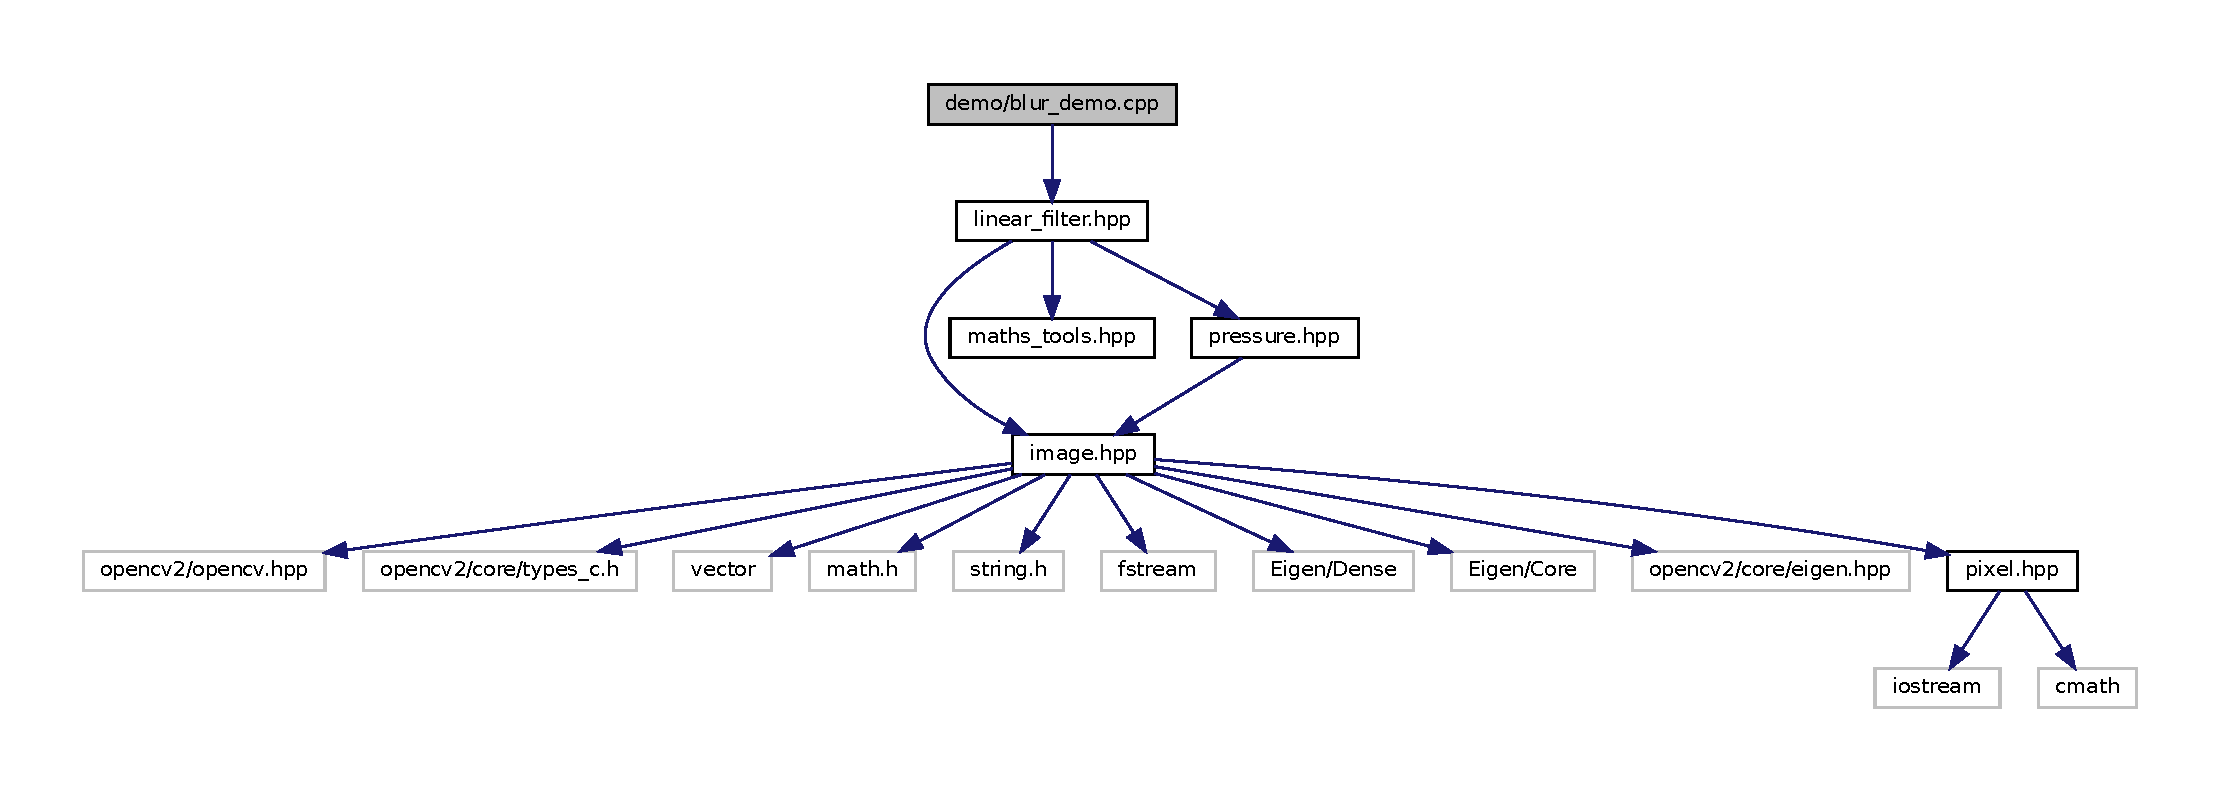
\includegraphics[width=350pt]{blur__demo_8cpp__incl}
\end{center}
\end{figure}
\subsection*{Functions}
\begin{DoxyCompactItemize}
\item 
int \hyperlink{blur__demo_8cpp_abf9e6b7e6f15df4b525a2e7705ba3089}{main} (int argc, char const $\ast$argv\mbox{[}$\,$\mbox{]})
\end{DoxyCompactItemize}


\subsection{Function Documentation}
\mbox{\Hypertarget{blur__demo_8cpp_abf9e6b7e6f15df4b525a2e7705ba3089}\label{blur__demo_8cpp_abf9e6b7e6f15df4b525a2e7705ba3089}} 
\index{blur\+\_\+demo.\+cpp@{blur\+\_\+demo.\+cpp}!main@{main}}
\index{main@{main}!blur\+\_\+demo.\+cpp@{blur\+\_\+demo.\+cpp}}
\subsubsection{\texorpdfstring{main()}{main()}}
{\footnotesize\ttfamily int main (\begin{DoxyParamCaption}\item[{int}]{argc,  }\item[{char const $\ast$}]{argv\mbox{[}$\,$\mbox{]} }\end{DoxyParamCaption})}


\hypertarget{convolution__demo_8cpp}{}\section{demo/convolution\+\_\+demo.cpp File Reference}
\label{convolution__demo_8cpp}\index{demo/convolution\+\_\+demo.\+cpp@{demo/convolution\+\_\+demo.\+cpp}}
{\ttfamily \#include \char`\"{}linear\+\_\+filter.\+hpp\char`\"{}}\newline
Include dependency graph for convolution\+\_\+demo.\+cpp\+:
\nopagebreak
\begin{figure}[H]
\begin{center}
\leavevmode
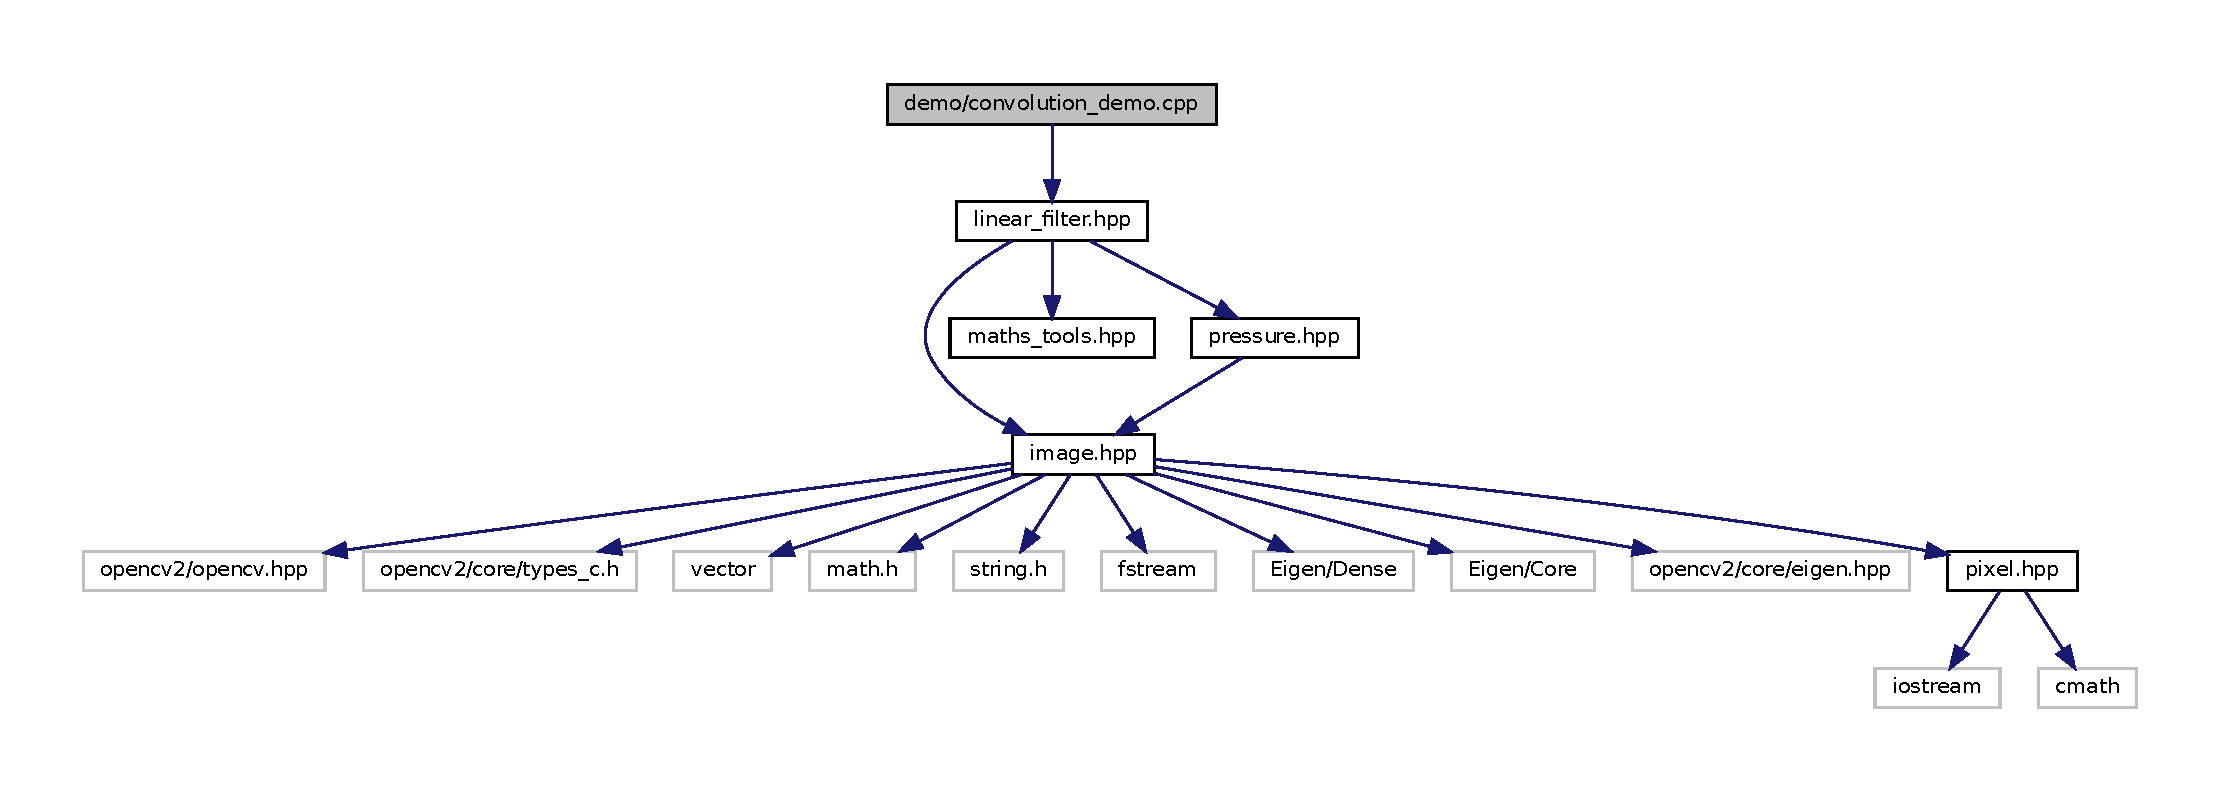
\includegraphics[width=350pt]{convolution__demo_8cpp__incl}
\end{center}
\end{figure}
\subsection*{Functions}
\begin{DoxyCompactItemize}
\item 
int \hyperlink{convolution__demo_8cpp_abf9e6b7e6f15df4b525a2e7705ba3089}{main} (int argc, char const $\ast$argv\mbox{[}$\,$\mbox{]})
\end{DoxyCompactItemize}


\subsection{Function Documentation}
\mbox{\Hypertarget{convolution__demo_8cpp_abf9e6b7e6f15df4b525a2e7705ba3089}\label{convolution__demo_8cpp_abf9e6b7e6f15df4b525a2e7705ba3089}} 
\index{convolution\+\_\+demo.\+cpp@{convolution\+\_\+demo.\+cpp}!main@{main}}
\index{main@{main}!convolution\+\_\+demo.\+cpp@{convolution\+\_\+demo.\+cpp}}
\subsubsection{\texorpdfstring{main()}{main()}}
{\footnotesize\ttfamily int main (\begin{DoxyParamCaption}\item[{int}]{argc,  }\item[{char const $\ast$}]{argv\mbox{[}$\,$\mbox{]} }\end{DoxyParamCaption})}


\hypertarget{demo__time__convolution_8cpp}{}\section{demo/demo\+\_\+time\+\_\+convolution.cpp File Reference}
\label{demo__time__convolution_8cpp}\index{demo/demo\+\_\+time\+\_\+convolution.\+cpp@{demo/demo\+\_\+time\+\_\+convolution.\+cpp}}
{\ttfamily \#include \char`\"{}linear\+\_\+filter.\+hpp\char`\"{}}\newline
Include dependency graph for demo\+\_\+time\+\_\+convolution.\+cpp\+:
\nopagebreak
\begin{figure}[H]
\begin{center}
\leavevmode
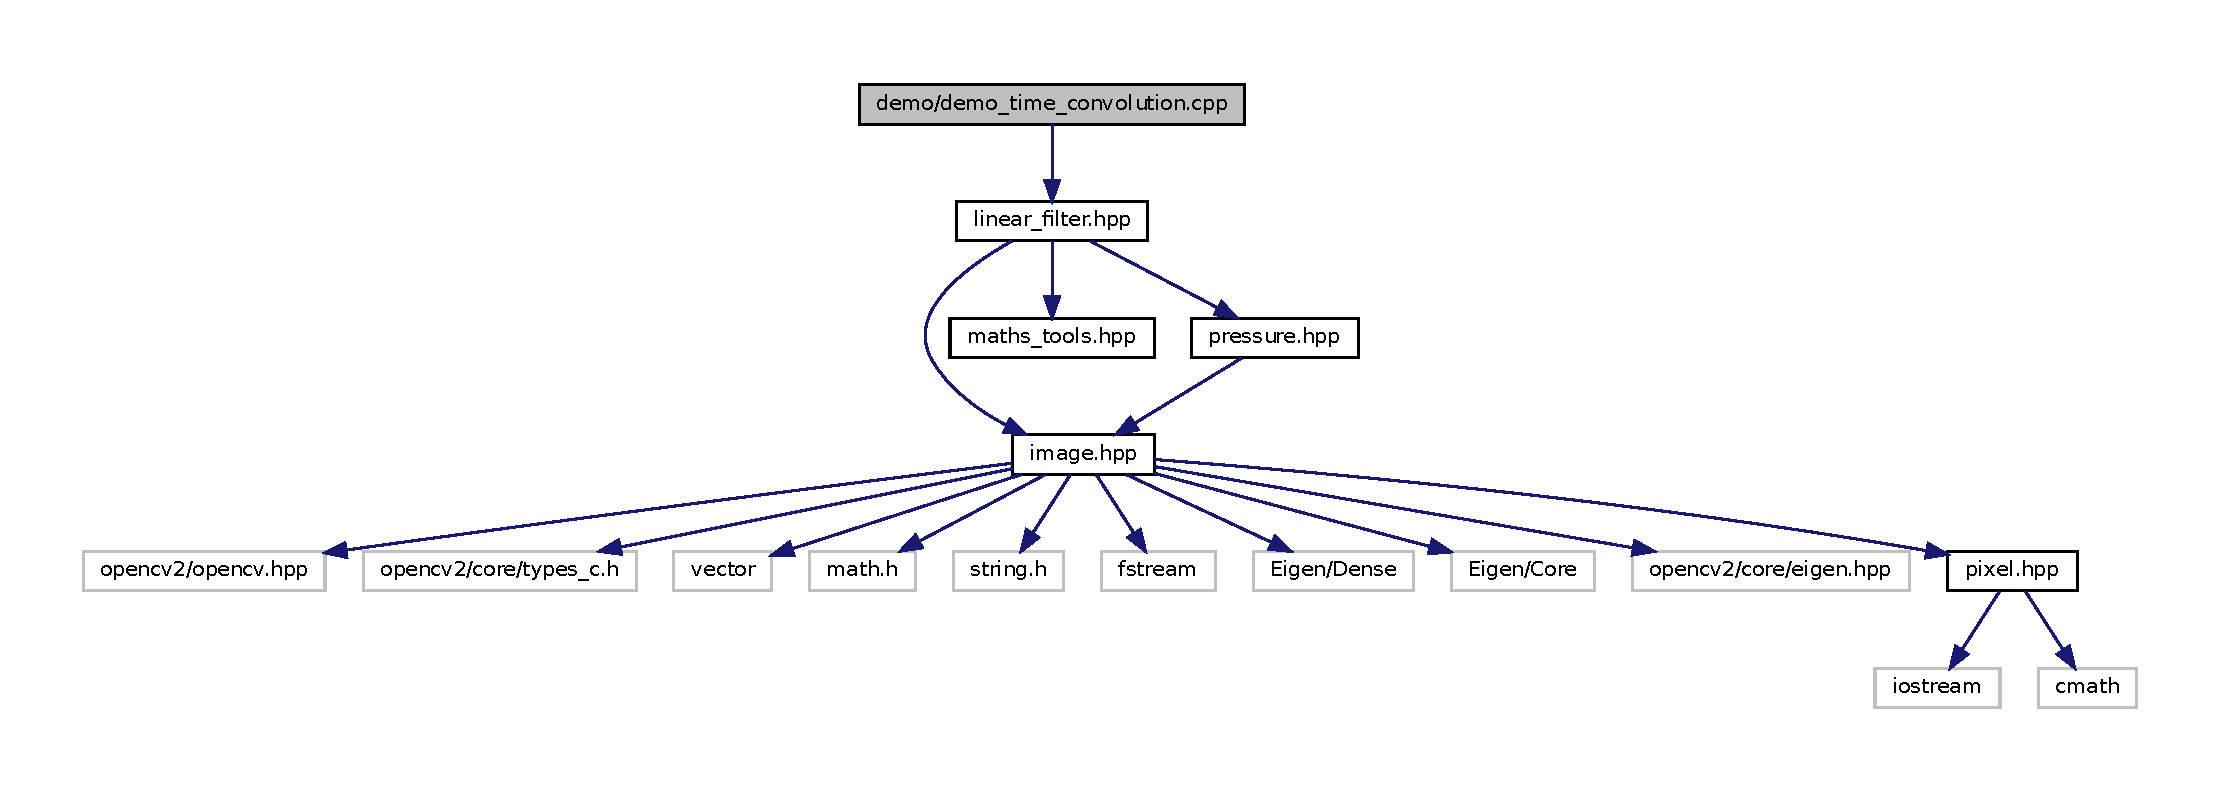
\includegraphics[width=350pt]{demo__time__convolution_8cpp__incl}
\end{center}
\end{figure}
\subsection*{Functions}
\begin{DoxyCompactItemize}
\item 
int \hyperlink{demo__time__convolution_8cpp_abf9e6b7e6f15df4b525a2e7705ba3089}{main} (int argc, char const $\ast$argv\mbox{[}$\,$\mbox{]})
\end{DoxyCompactItemize}


\subsection{Function Documentation}
\mbox{\Hypertarget{demo__time__convolution_8cpp_abf9e6b7e6f15df4b525a2e7705ba3089}\label{demo__time__convolution_8cpp_abf9e6b7e6f15df4b525a2e7705ba3089}} 
\index{demo\+\_\+time\+\_\+convolution.\+cpp@{demo\+\_\+time\+\_\+convolution.\+cpp}!main@{main}}
\index{main@{main}!demo\+\_\+time\+\_\+convolution.\+cpp@{demo\+\_\+time\+\_\+convolution.\+cpp}}
\subsubsection{\texorpdfstring{main()}{main()}}
{\footnotesize\ttfamily int main (\begin{DoxyParamCaption}\item[{int}]{argc,  }\item[{char const $\ast$}]{argv\mbox{[}$\,$\mbox{]} }\end{DoxyParamCaption})}


\hypertarget{dft__convolution__demo_8cpp}{}\section{demo/dft\+\_\+convolution\+\_\+demo.cpp File Reference}
\label{dft__convolution__demo_8cpp}\index{demo/dft\+\_\+convolution\+\_\+demo.\+cpp@{demo/dft\+\_\+convolution\+\_\+demo.\+cpp}}
{\ttfamily \#include \char`\"{}linear\+\_\+filter.\+hpp\char`\"{}}\newline
Include dependency graph for dft\+\_\+convolution\+\_\+demo.\+cpp\+:
\nopagebreak
\begin{figure}[H]
\begin{center}
\leavevmode
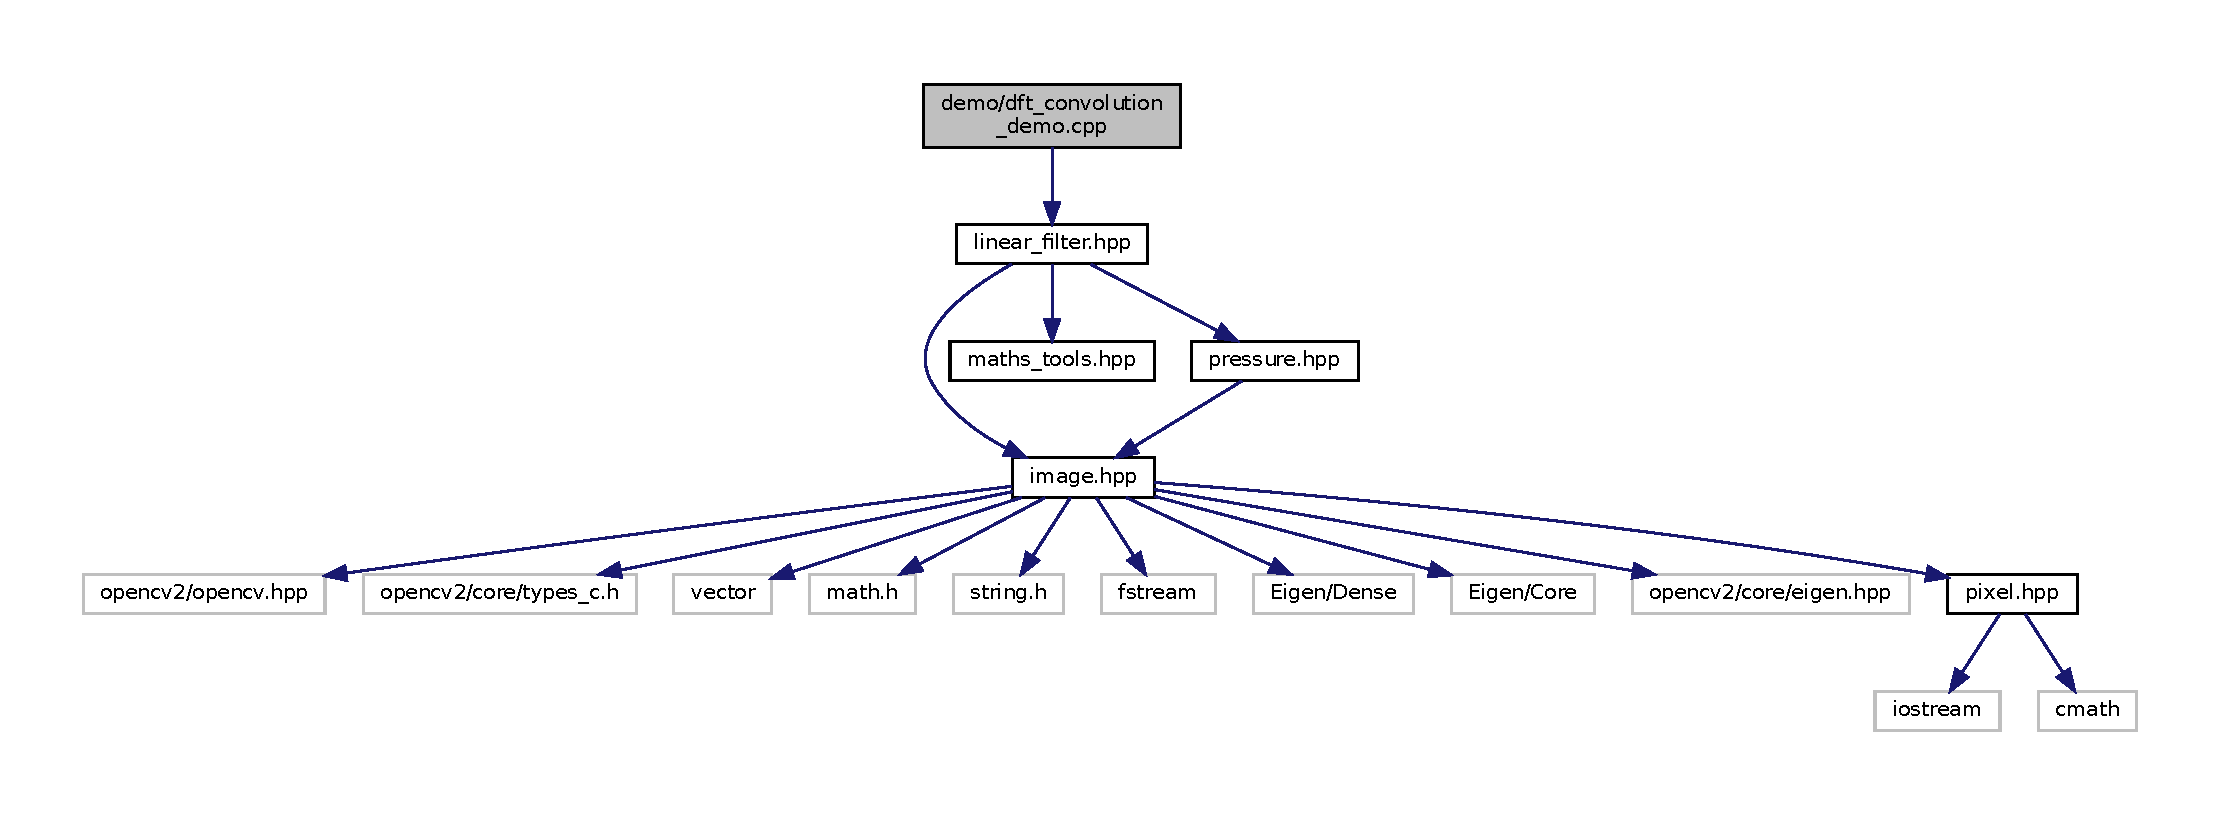
\includegraphics[width=350pt]{dft__convolution__demo_8cpp__incl}
\end{center}
\end{figure}
\subsection*{Functions}
\begin{DoxyCompactItemize}
\item 
int \hyperlink{dft__convolution__demo_8cpp_abf9e6b7e6f15df4b525a2e7705ba3089}{main} (int argc, char const $\ast$argv\mbox{[}$\,$\mbox{]})
\end{DoxyCompactItemize}


\subsection{Function Documentation}
\mbox{\Hypertarget{dft__convolution__demo_8cpp_abf9e6b7e6f15df4b525a2e7705ba3089}\label{dft__convolution__demo_8cpp_abf9e6b7e6f15df4b525a2e7705ba3089}} 
\index{dft\+\_\+convolution\+\_\+demo.\+cpp@{dft\+\_\+convolution\+\_\+demo.\+cpp}!main@{main}}
\index{main@{main}!dft\+\_\+convolution\+\_\+demo.\+cpp@{dft\+\_\+convolution\+\_\+demo.\+cpp}}
\subsubsection{\texorpdfstring{main()}{main()}}
{\footnotesize\ttfamily int main (\begin{DoxyParamCaption}\item[{int}]{argc,  }\item[{char const $\ast$}]{argv\mbox{[}$\,$\mbox{]} }\end{DoxyParamCaption})}


\hypertarget{image__demo_8cpp}{}\section{demo/image\+\_\+demo.cpp File Reference}
\label{image__demo_8cpp}\index{demo/image\+\_\+demo.\+cpp@{demo/image\+\_\+demo.\+cpp}}
{\ttfamily \#include \char`\"{}image.\+hpp\char`\"{}}\newline
Include dependency graph for image\+\_\+demo.\+cpp\+:
\nopagebreak
\begin{figure}[H]
\begin{center}
\leavevmode
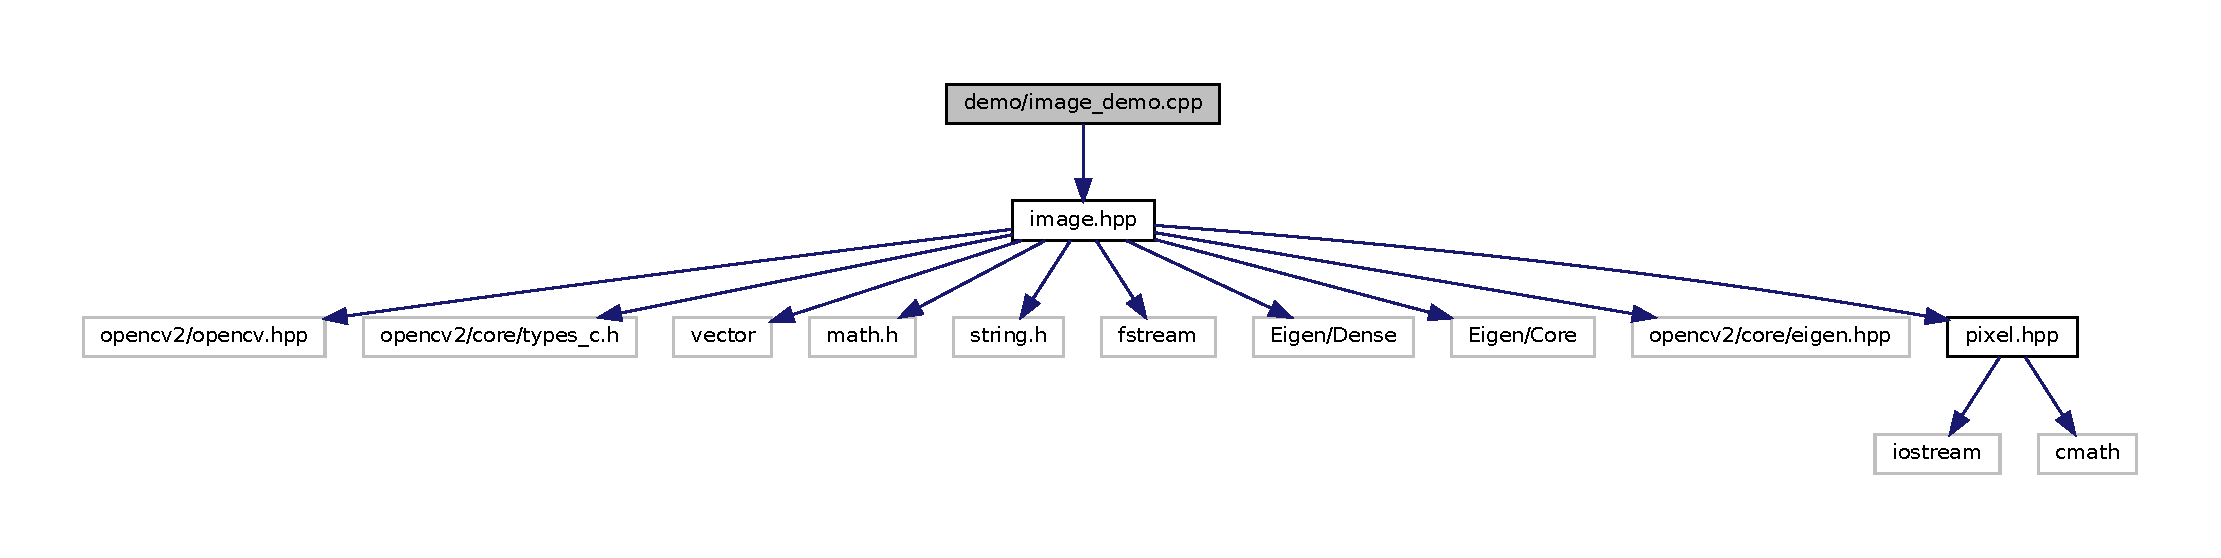
\includegraphics[width=350pt]{image__demo_8cpp__incl}
\end{center}
\end{figure}
\subsection*{Functions}
\begin{DoxyCompactItemize}
\item 
int \hyperlink{image__demo_8cpp_abf9e6b7e6f15df4b525a2e7705ba3089}{main} (int argc, char const $\ast$argv\mbox{[}$\,$\mbox{]})
\end{DoxyCompactItemize}


\subsection{Function Documentation}
\mbox{\Hypertarget{image__demo_8cpp_abf9e6b7e6f15df4b525a2e7705ba3089}\label{image__demo_8cpp_abf9e6b7e6f15df4b525a2e7705ba3089}} 
\index{image\+\_\+demo.\+cpp@{image\+\_\+demo.\+cpp}!main@{main}}
\index{main@{main}!image\+\_\+demo.\+cpp@{image\+\_\+demo.\+cpp}}
\subsubsection{\texorpdfstring{main()}{main()}}
{\footnotesize\ttfamily int main (\begin{DoxyParamCaption}\item[{int}]{argc,  }\item[{char const $\ast$}]{argv\mbox{[}$\,$\mbox{]} }\end{DoxyParamCaption})}


\hypertarget{optimization__rtxy__demo_8cpp}{}\section{demo/optimization\+\_\+rtxy\+\_\+demo.cpp File Reference}
\label{optimization__rtxy__demo_8cpp}\index{demo/optimization\+\_\+rtxy\+\_\+demo.\+cpp@{demo/optimization\+\_\+rtxy\+\_\+demo.\+cpp}}
{\ttfamily \#include \char`\"{}image.\+hpp\char`\"{}}\newline
Include dependency graph for optimization\+\_\+rtxy\+\_\+demo.\+cpp\+:
\nopagebreak
\begin{figure}[H]
\begin{center}
\leavevmode
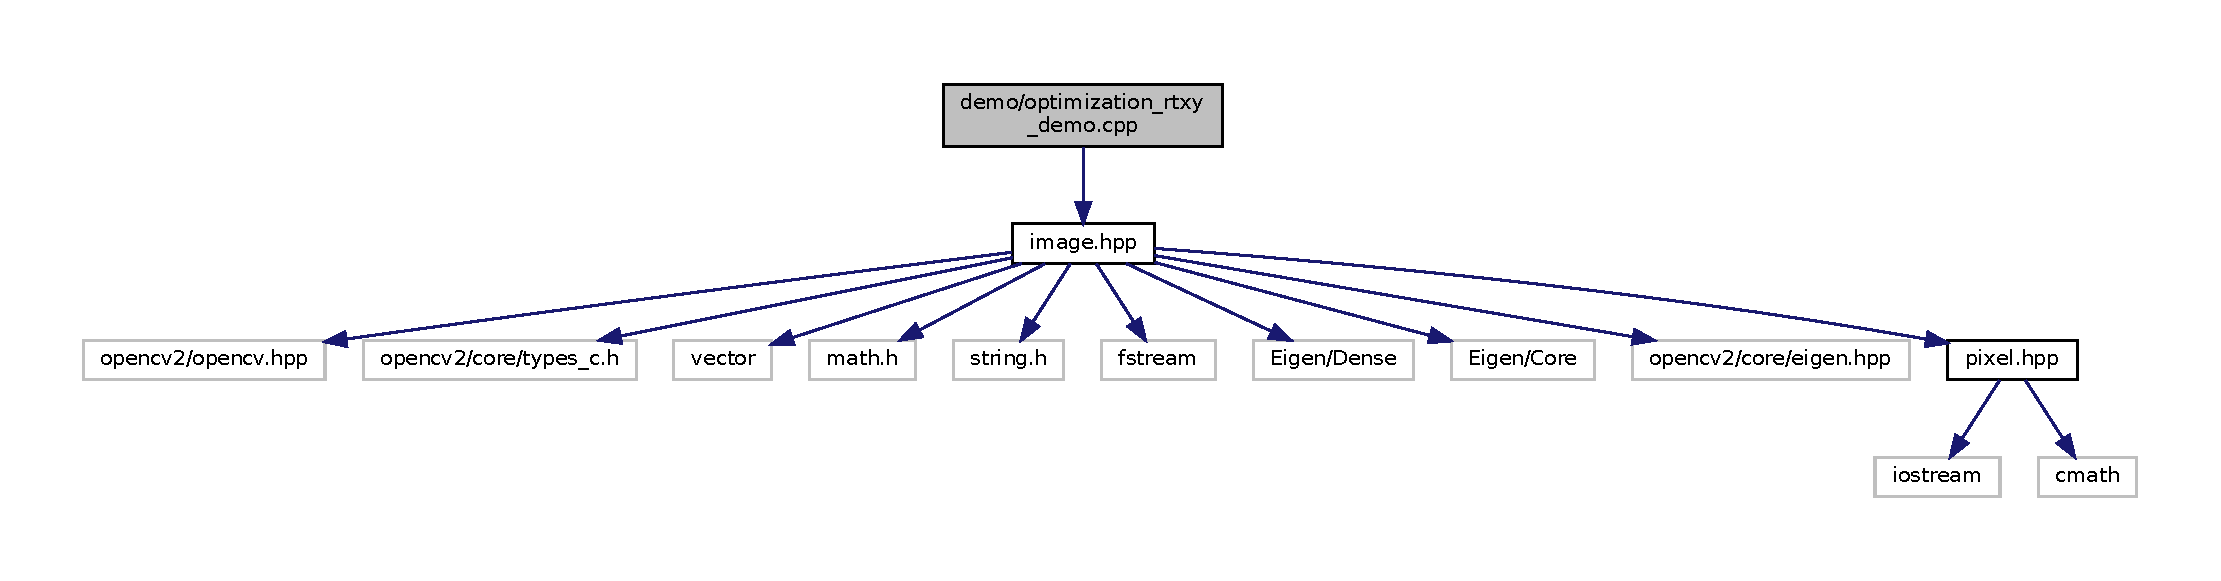
\includegraphics[width=350pt]{optimization__rtxy__demo_8cpp__incl}
\end{center}
\end{figure}
\subsection*{Functions}
\begin{DoxyCompactItemize}
\item 
int \hyperlink{optimization__rtxy__demo_8cpp_abf9e6b7e6f15df4b525a2e7705ba3089}{main} (int argc, char const $\ast$argv\mbox{[}$\,$\mbox{]})
\end{DoxyCompactItemize}


\subsection{Function Documentation}
\mbox{\Hypertarget{optimization__rtxy__demo_8cpp_abf9e6b7e6f15df4b525a2e7705ba3089}\label{optimization__rtxy__demo_8cpp_abf9e6b7e6f15df4b525a2e7705ba3089}} 
\index{optimization\+\_\+rtxy\+\_\+demo.\+cpp@{optimization\+\_\+rtxy\+\_\+demo.\+cpp}!main@{main}}
\index{main@{main}!optimization\+\_\+rtxy\+\_\+demo.\+cpp@{optimization\+\_\+rtxy\+\_\+demo.\+cpp}}
\subsubsection{\texorpdfstring{main()}{main()}}
{\footnotesize\ttfamily int main (\begin{DoxyParamCaption}\item[{int}]{argc,  }\item[{char const $\ast$}]{argv\mbox{[}$\,$\mbox{]} }\end{DoxyParamCaption})}


\hypertarget{optimization__tx__demo_8cpp}{}\section{demo/optimization\+\_\+tx\+\_\+demo.cpp File Reference}
\label{optimization__tx__demo_8cpp}\index{demo/optimization\+\_\+tx\+\_\+demo.\+cpp@{demo/optimization\+\_\+tx\+\_\+demo.\+cpp}}
{\ttfamily \#include \char`\"{}image.\+hpp\char`\"{}}\newline
Include dependency graph for optimization\+\_\+tx\+\_\+demo.\+cpp\+:
\nopagebreak
\begin{figure}[H]
\begin{center}
\leavevmode
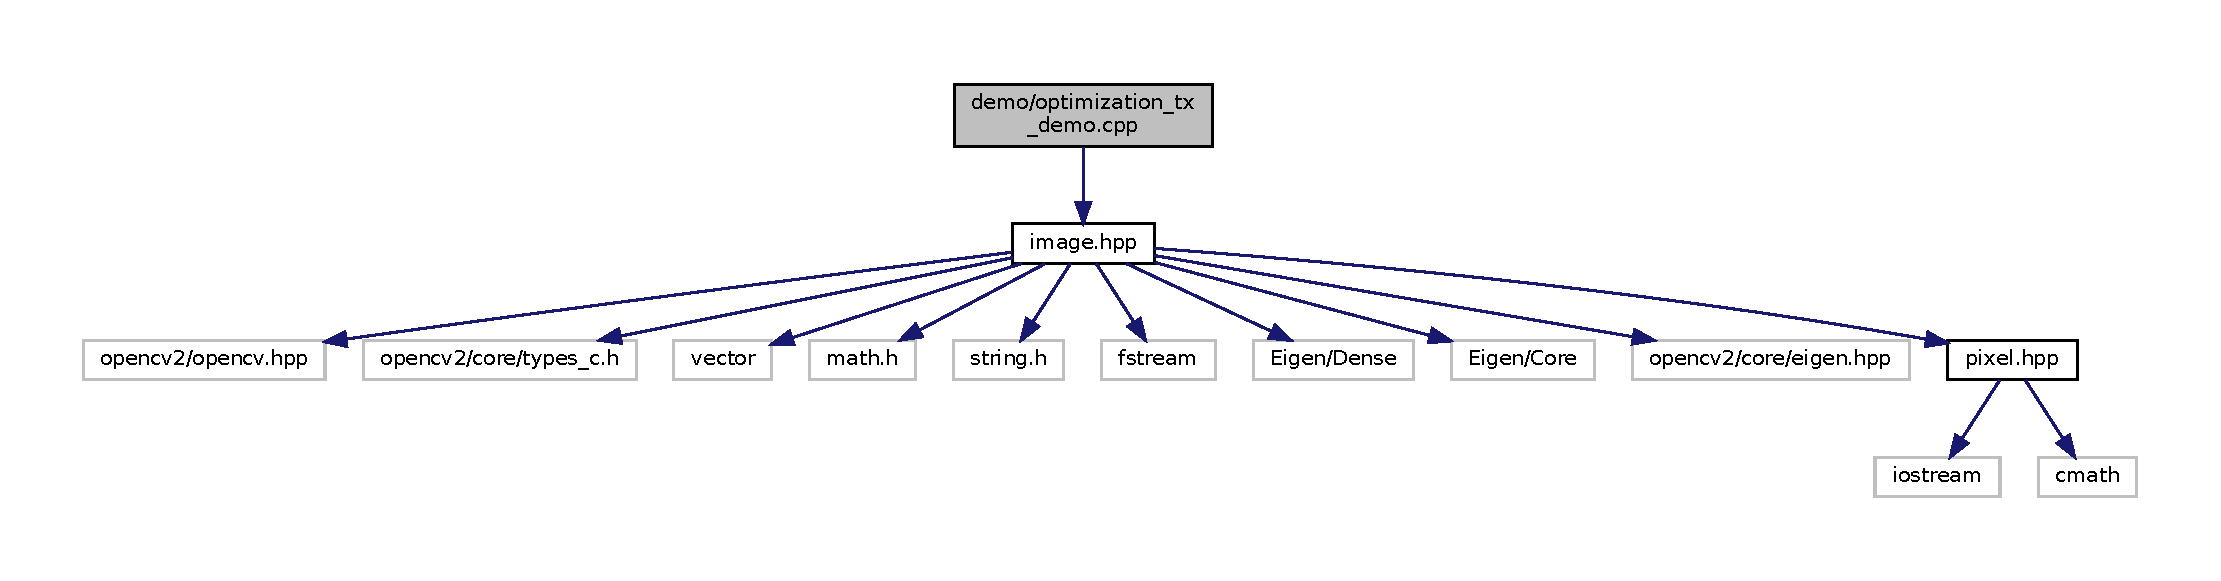
\includegraphics[width=350pt]{optimization__tx__demo_8cpp__incl}
\end{center}
\end{figure}
\subsection*{Functions}
\begin{DoxyCompactItemize}
\item 
int \hyperlink{optimization__tx__demo_8cpp_abf9e6b7e6f15df4b525a2e7705ba3089}{main} (int argc, char const $\ast$argv\mbox{[}$\,$\mbox{]})
\end{DoxyCompactItemize}


\subsection{Function Documentation}
\mbox{\Hypertarget{optimization__tx__demo_8cpp_abf9e6b7e6f15df4b525a2e7705ba3089}\label{optimization__tx__demo_8cpp_abf9e6b7e6f15df4b525a2e7705ba3089}} 
\index{optimization\+\_\+tx\+\_\+demo.\+cpp@{optimization\+\_\+tx\+\_\+demo.\+cpp}!main@{main}}
\index{main@{main}!optimization\+\_\+tx\+\_\+demo.\+cpp@{optimization\+\_\+tx\+\_\+demo.\+cpp}}
\subsubsection{\texorpdfstring{main()}{main()}}
{\footnotesize\ttfamily int main (\begin{DoxyParamCaption}\item[{int}]{argc,  }\item[{char const $\ast$}]{argv\mbox{[}$\,$\mbox{]} }\end{DoxyParamCaption})}


\hypertarget{optimization__txy__demo_8cpp}{}\section{demo/optimization\+\_\+txy\+\_\+demo.cpp File Reference}
\label{optimization__txy__demo_8cpp}\index{demo/optimization\+\_\+txy\+\_\+demo.\+cpp@{demo/optimization\+\_\+txy\+\_\+demo.\+cpp}}
{\ttfamily \#include \char`\"{}image.\+hpp\char`\"{}}\newline
Include dependency graph for optimization\+\_\+txy\+\_\+demo.\+cpp\+:
\nopagebreak
\begin{figure}[H]
\begin{center}
\leavevmode
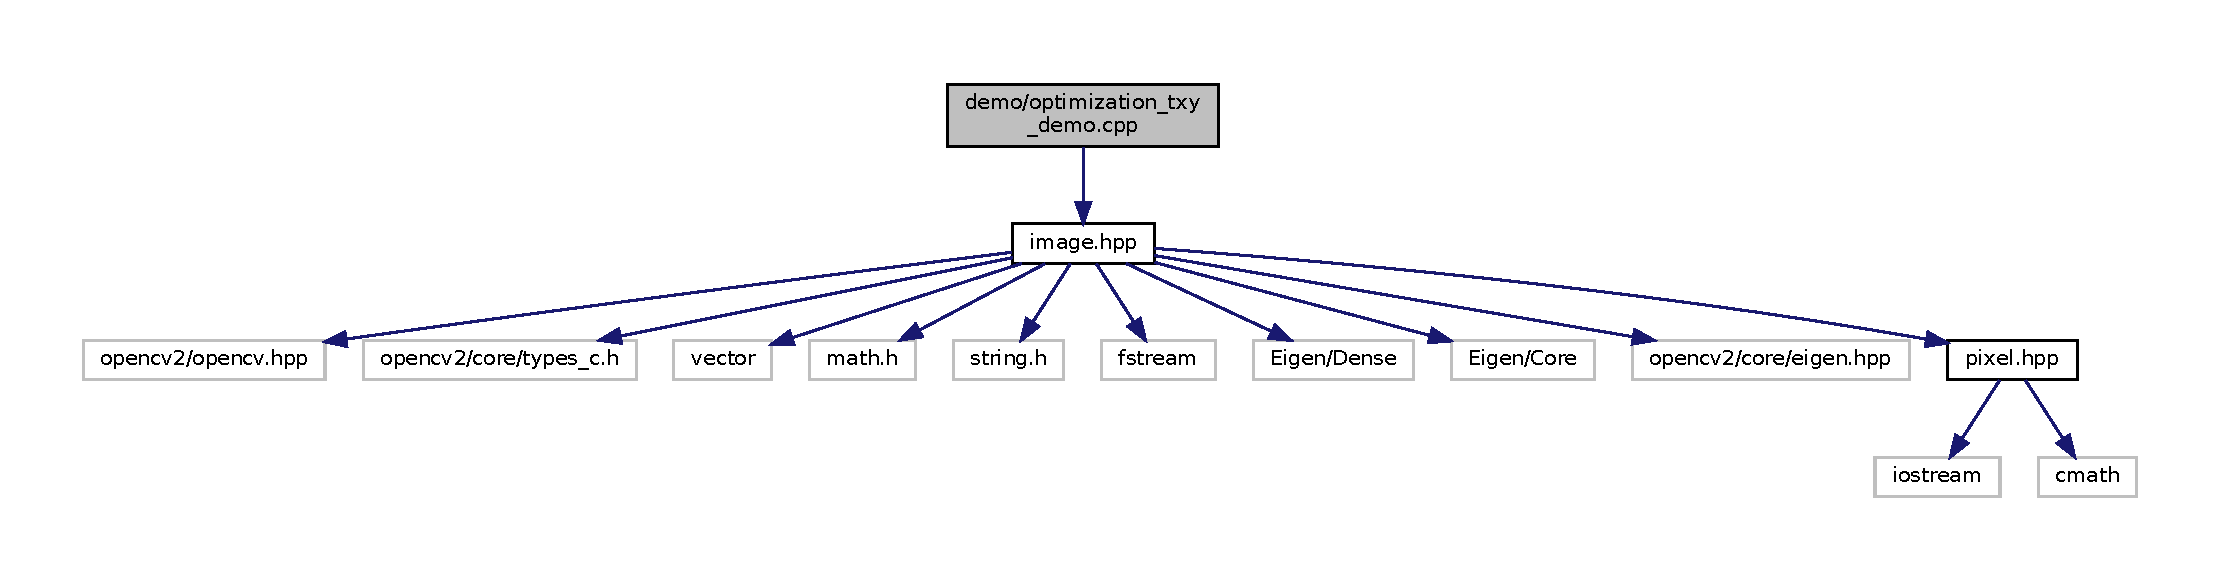
\includegraphics[width=350pt]{optimization__txy__demo_8cpp__incl}
\end{center}
\end{figure}
\subsection*{Functions}
\begin{DoxyCompactItemize}
\item 
int \hyperlink{optimization__txy__demo_8cpp_abf9e6b7e6f15df4b525a2e7705ba3089}{main} (int argc, char const $\ast$argv\mbox{[}$\,$\mbox{]})
\end{DoxyCompactItemize}


\subsection{Function Documentation}
\mbox{\Hypertarget{optimization__txy__demo_8cpp_abf9e6b7e6f15df4b525a2e7705ba3089}\label{optimization__txy__demo_8cpp_abf9e6b7e6f15df4b525a2e7705ba3089}} 
\index{optimization\+\_\+txy\+\_\+demo.\+cpp@{optimization\+\_\+txy\+\_\+demo.\+cpp}!main@{main}}
\index{main@{main}!optimization\+\_\+txy\+\_\+demo.\+cpp@{optimization\+\_\+txy\+\_\+demo.\+cpp}}
\subsubsection{\texorpdfstring{main()}{main()}}
{\footnotesize\ttfamily int main (\begin{DoxyParamCaption}\item[{int}]{argc,  }\item[{char const $\ast$}]{argv\mbox{[}$\,$\mbox{]} }\end{DoxyParamCaption})}


\hypertarget{pressure__demo_8cpp}{}\section{demo/pressure\+\_\+demo.cpp File Reference}
\label{pressure__demo_8cpp}\index{demo/pressure\+\_\+demo.\+cpp@{demo/pressure\+\_\+demo.\+cpp}}
{\ttfamily \#include \char`\"{}image.\+hpp\char`\"{}}\newline
Include dependency graph for pressure\+\_\+demo.\+cpp\+:
\nopagebreak
\begin{figure}[H]
\begin{center}
\leavevmode
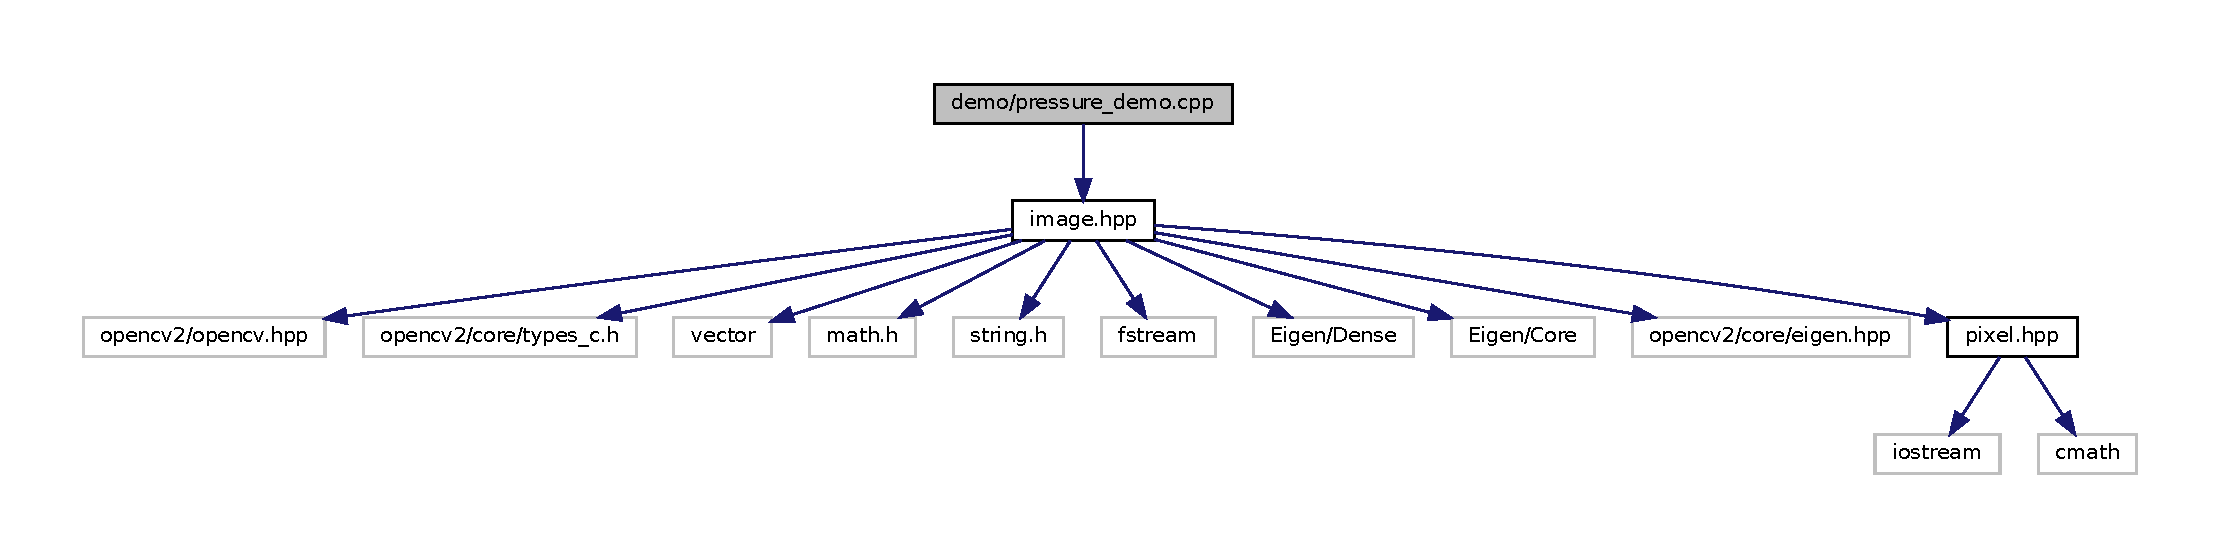
\includegraphics[width=350pt]{pressure__demo_8cpp__incl}
\end{center}
\end{figure}
\subsection*{Functions}
\begin{DoxyCompactItemize}
\item 
int \hyperlink{pressure__demo_8cpp_abf9e6b7e6f15df4b525a2e7705ba3089}{main} (int argc, char const $\ast$argv\mbox{[}$\,$\mbox{]})
\end{DoxyCompactItemize}


\subsection{Function Documentation}
\mbox{\Hypertarget{pressure__demo_8cpp_abf9e6b7e6f15df4b525a2e7705ba3089}\label{pressure__demo_8cpp_abf9e6b7e6f15df4b525a2e7705ba3089}} 
\index{pressure\+\_\+demo.\+cpp@{pressure\+\_\+demo.\+cpp}!main@{main}}
\index{main@{main}!pressure\+\_\+demo.\+cpp@{pressure\+\_\+demo.\+cpp}}
\subsubsection{\texorpdfstring{main()}{main()}}
{\footnotesize\ttfamily int main (\begin{DoxyParamCaption}\item[{int}]{argc,  }\item[{char const $\ast$}]{argv\mbox{[}$\,$\mbox{]} }\end{DoxyParamCaption})}


\hypertarget{rotation__comp__demo_8cpp}{}\section{demo/rotation\+\_\+comp\+\_\+demo.cpp File Reference}
\label{rotation__comp__demo_8cpp}\index{demo/rotation\+\_\+comp\+\_\+demo.\+cpp@{demo/rotation\+\_\+comp\+\_\+demo.\+cpp}}
{\ttfamily \#include \char`\"{}image.\+hpp\char`\"{}}\newline
Include dependency graph for rotation\+\_\+comp\+\_\+demo.\+cpp\+:
\nopagebreak
\begin{figure}[H]
\begin{center}
\leavevmode
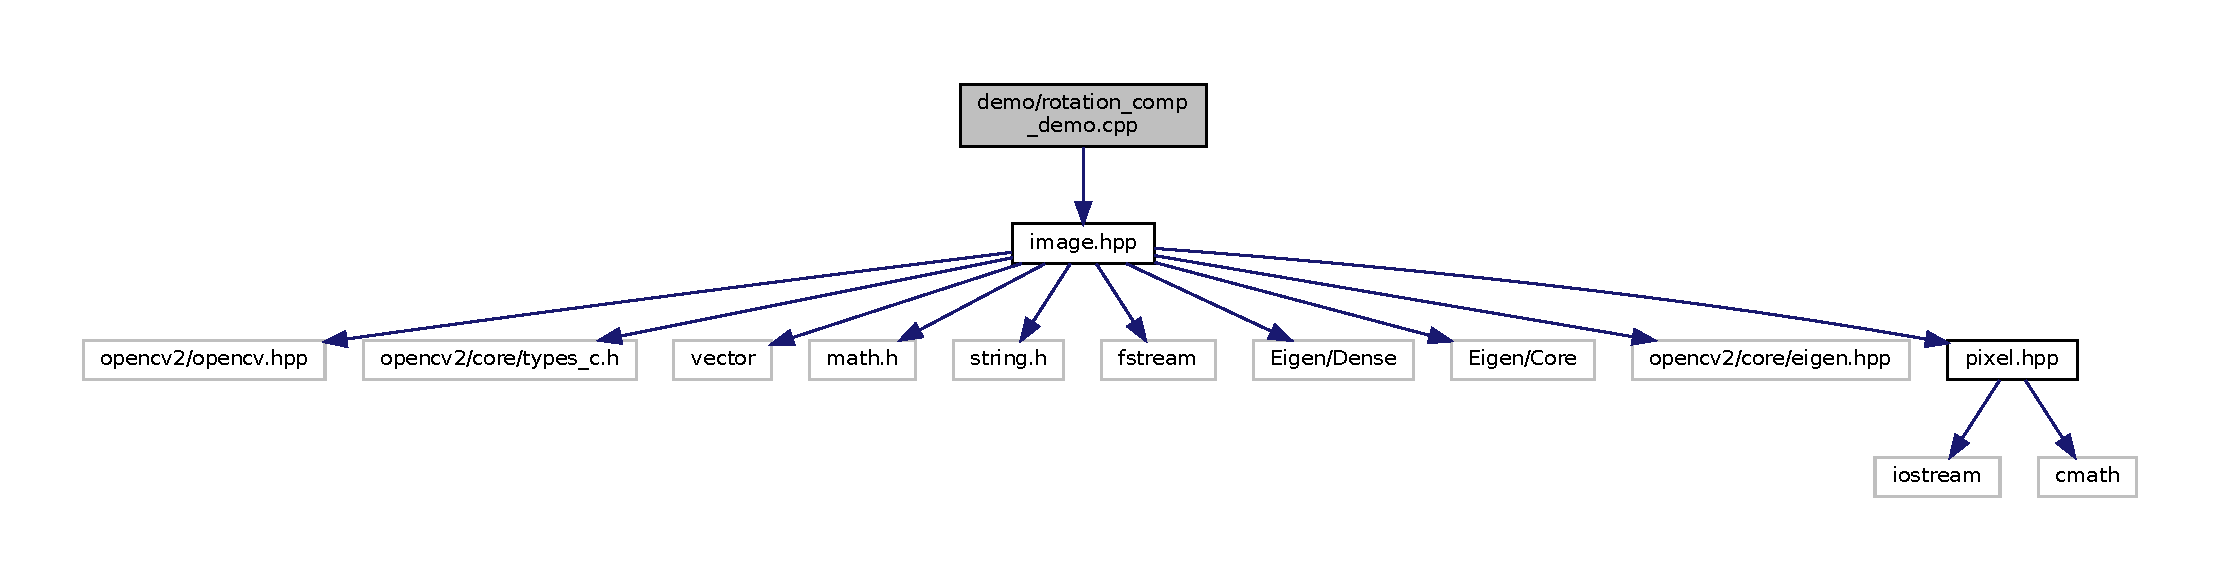
\includegraphics[width=350pt]{rotation__comp__demo_8cpp__incl}
\end{center}
\end{figure}
\subsection*{Functions}
\begin{DoxyCompactItemize}
\item 
int \hyperlink{rotation__comp__demo_8cpp_abf9e6b7e6f15df4b525a2e7705ba3089}{main} (int argc, char const $\ast$argv\mbox{[}$\,$\mbox{]})
\end{DoxyCompactItemize}


\subsection{Function Documentation}
\mbox{\Hypertarget{rotation__comp__demo_8cpp_abf9e6b7e6f15df4b525a2e7705ba3089}\label{rotation__comp__demo_8cpp_abf9e6b7e6f15df4b525a2e7705ba3089}} 
\index{rotation\+\_\+comp\+\_\+demo.\+cpp@{rotation\+\_\+comp\+\_\+demo.\+cpp}!main@{main}}
\index{main@{main}!rotation\+\_\+comp\+\_\+demo.\+cpp@{rotation\+\_\+comp\+\_\+demo.\+cpp}}
\subsubsection{\texorpdfstring{main()}{main()}}
{\footnotesize\ttfamily int main (\begin{DoxyParamCaption}\item[{int}]{argc,  }\item[{char const $\ast$}]{argv\mbox{[}$\,$\mbox{]} }\end{DoxyParamCaption})}


\hypertarget{rotation__demo_8cpp}{}\section{demo/rotation\+\_\+demo.cpp File Reference}
\label{rotation__demo_8cpp}\index{demo/rotation\+\_\+demo.\+cpp@{demo/rotation\+\_\+demo.\+cpp}}
{\ttfamily \#include \char`\"{}image.\+hpp\char`\"{}}\newline
Include dependency graph for rotation\+\_\+demo.\+cpp\+:
\nopagebreak
\begin{figure}[H]
\begin{center}
\leavevmode
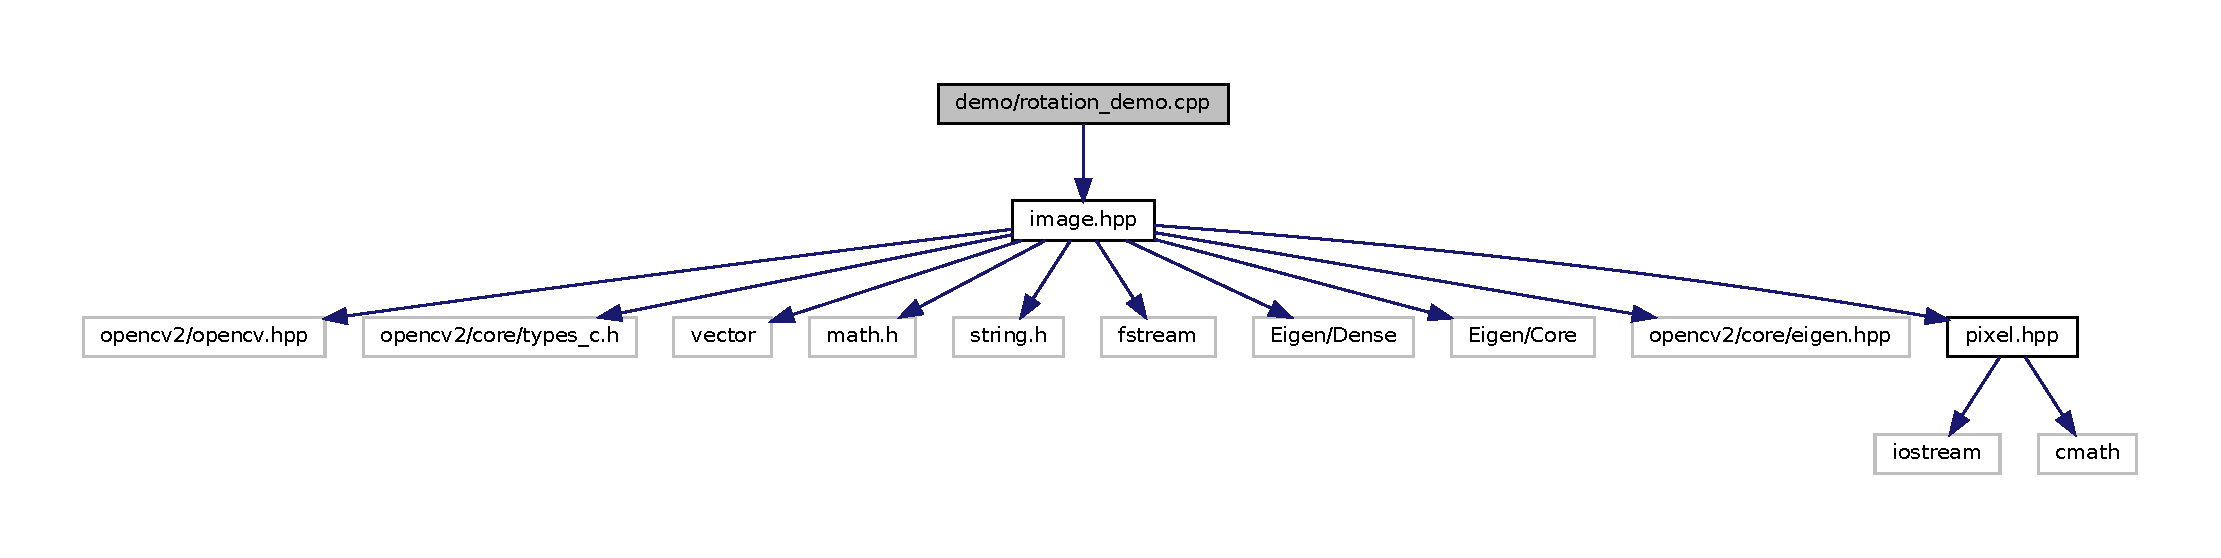
\includegraphics[width=350pt]{rotation__demo_8cpp__incl}
\end{center}
\end{figure}
\subsection*{Functions}
\begin{DoxyCompactItemize}
\item 
int \hyperlink{rotation__demo_8cpp_abf9e6b7e6f15df4b525a2e7705ba3089}{main} (int argc, char const $\ast$argv\mbox{[}$\,$\mbox{]})
\end{DoxyCompactItemize}


\subsection{Function Documentation}
\mbox{\Hypertarget{rotation__demo_8cpp_abf9e6b7e6f15df4b525a2e7705ba3089}\label{rotation__demo_8cpp_abf9e6b7e6f15df4b525a2e7705ba3089}} 
\index{rotation\+\_\+demo.\+cpp@{rotation\+\_\+demo.\+cpp}!main@{main}}
\index{main@{main}!rotation\+\_\+demo.\+cpp@{rotation\+\_\+demo.\+cpp}}
\subsubsection{\texorpdfstring{main()}{main()}}
{\footnotesize\ttfamily int main (\begin{DoxyParamCaption}\item[{int}]{argc,  }\item[{char const $\ast$}]{argv\mbox{[}$\,$\mbox{]} }\end{DoxyParamCaption})}


\hypertarget{warp__demo_8cpp}{}\section{demo/warp\+\_\+demo.cpp File Reference}
\label{warp__demo_8cpp}\index{demo/warp\+\_\+demo.\+cpp@{demo/warp\+\_\+demo.\+cpp}}
{\ttfamily \#include \char`\"{}image.\+hpp\char`\"{}}\newline
Include dependency graph for warp\+\_\+demo.\+cpp\+:
\nopagebreak
\begin{figure}[H]
\begin{center}
\leavevmode
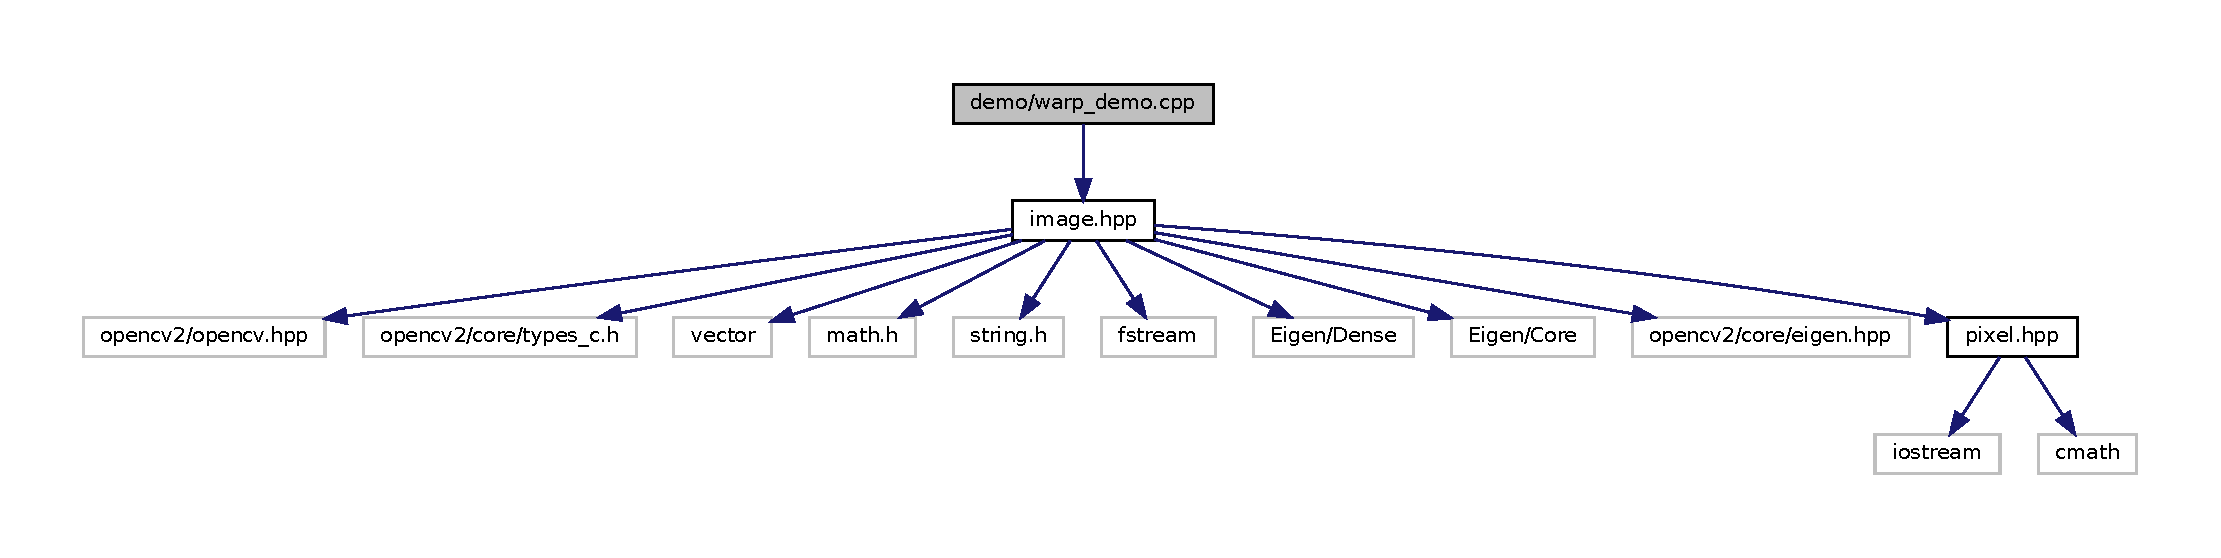
\includegraphics[width=350pt]{warp__demo_8cpp__incl}
\end{center}
\end{figure}
\subsection*{Functions}
\begin{DoxyCompactItemize}
\item 
int \hyperlink{warp__demo_8cpp_abf9e6b7e6f15df4b525a2e7705ba3089}{main} (int argc, char const $\ast$argv\mbox{[}$\,$\mbox{]})
\end{DoxyCompactItemize}


\subsection{Function Documentation}
\mbox{\Hypertarget{warp__demo_8cpp_abf9e6b7e6f15df4b525a2e7705ba3089}\label{warp__demo_8cpp_abf9e6b7e6f15df4b525a2e7705ba3089}} 
\index{warp\+\_\+demo.\+cpp@{warp\+\_\+demo.\+cpp}!main@{main}}
\index{main@{main}!warp\+\_\+demo.\+cpp@{warp\+\_\+demo.\+cpp}}
\subsubsection{\texorpdfstring{main()}{main()}}
{\footnotesize\ttfamily int main (\begin{DoxyParamCaption}\item[{int}]{argc,  }\item[{char const $\ast$}]{argv\mbox{[}$\,$\mbox{]} }\end{DoxyParamCaption})}


\hypertarget{image_8hpp}{}\section{inc/image.hpp File Reference}
\label{image_8hpp}\index{inc/image.\+hpp@{inc/image.\+hpp}}


Definition of \hyperlink{class_image}{Image} class.  


{\ttfamily \#include $<$opencv2/opencv.\+hpp$>$}\newline
{\ttfamily \#include $<$opencv2/core/types\+\_\+c.\+h$>$}\newline
{\ttfamily \#include $<$vector$>$}\newline
{\ttfamily \#include $<$math.\+h$>$}\newline
{\ttfamily \#include $<$string.\+h$>$}\newline
{\ttfamily \#include $<$fstream$>$}\newline
{\ttfamily \#include $<$Eigen/\+Dense$>$}\newline
{\ttfamily \#include $<$Eigen/\+Core$>$}\newline
{\ttfamily \#include $<$opencv2/core/eigen.\+hpp$>$}\newline
{\ttfamily \#include \char`\"{}pixel.\+hpp\char`\"{}}\newline
Include dependency graph for image.\+hpp\+:
\nopagebreak
\begin{figure}[H]
\begin{center}
\leavevmode
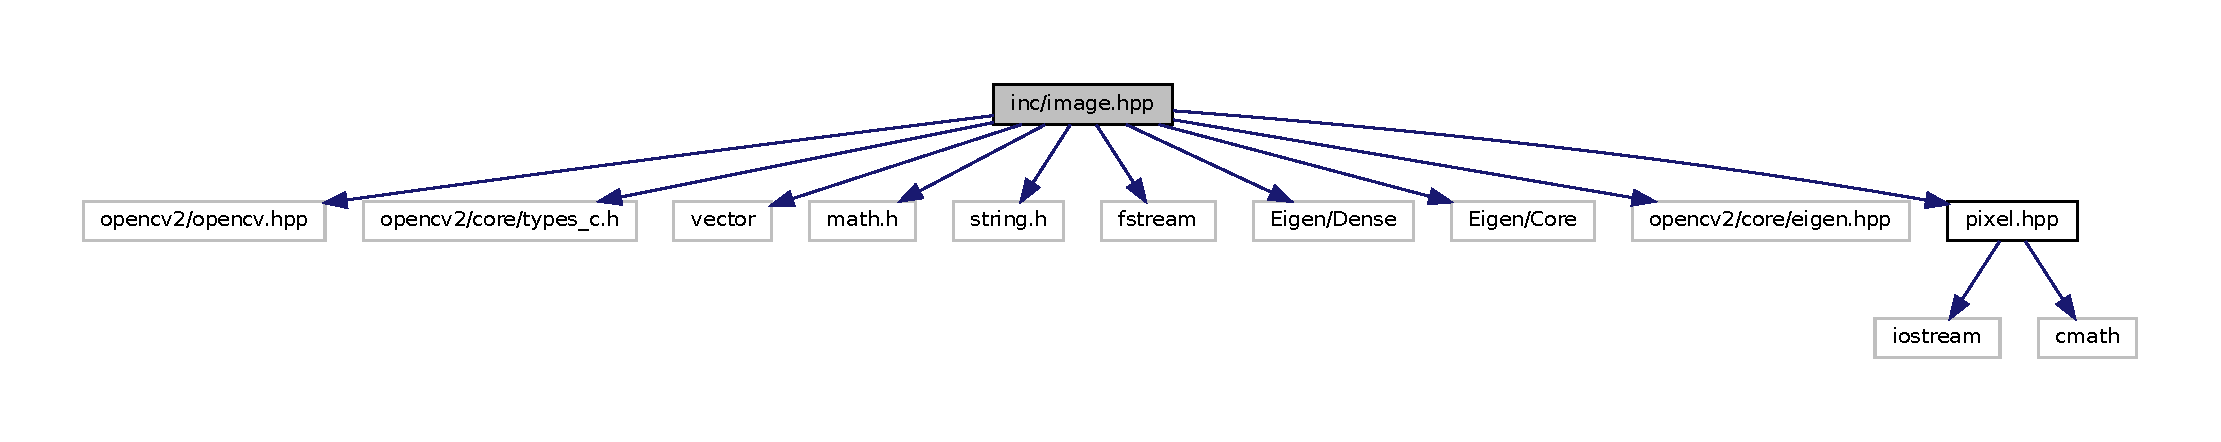
\includegraphics[width=350pt]{image_8hpp__incl}
\end{center}
\end{figure}
This graph shows which files directly or indirectly include this file\+:
\nopagebreak
\begin{figure}[H]
\begin{center}
\leavevmode
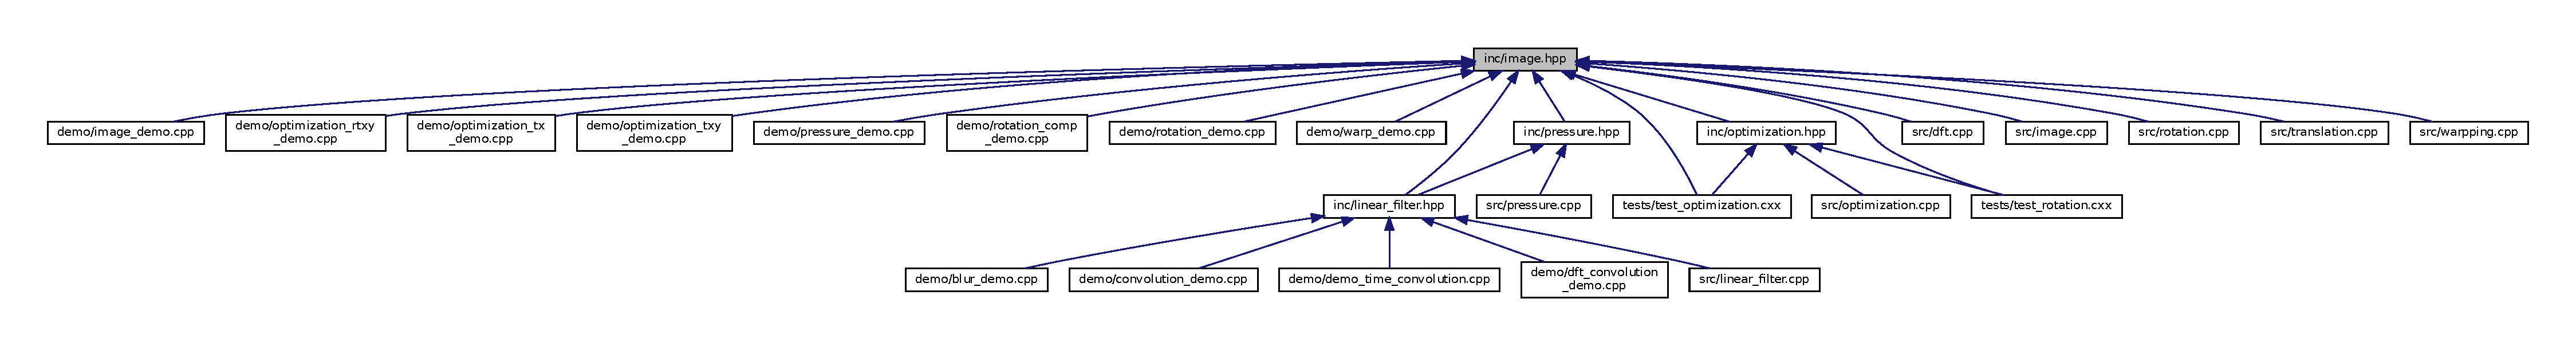
\includegraphics[width=350pt]{image_8hpp__dep__incl}
\end{center}
\end{figure}
\subsection*{Classes}
\begin{DoxyCompactItemize}
\item 
class \hyperlink{class_image}{Image}
\begin{DoxyCompactList}\small\item\em class of the image we\textquotesingle{}ll work on \end{DoxyCompactList}\end{DoxyCompactItemize}


\subsection{Detailed Description}
Definition of \hyperlink{class_image}{Image} class. 

\begin{DoxyAuthor}{Author}
Perrine, Célestine, Aurélien, Lucas 
\end{DoxyAuthor}

\hypertarget{linear__filter_8hpp}{}\section{inc/linear\+\_\+filter.hpp File Reference}
\label{linear__filter_8hpp}\index{inc/linear\+\_\+filter.\+hpp@{inc/linear\+\_\+filter.\+hpp}}
{\ttfamily \#include \char`\"{}image.\+hpp\char`\"{}}\newline
{\ttfamily \#include \char`\"{}maths\+\_\+tools.\+hpp\char`\"{}}\newline
{\ttfamily \#include \char`\"{}pressure.\+hpp\char`\"{}}\newline
Include dependency graph for linear\+\_\+filter.\+hpp\+:
\nopagebreak
\begin{figure}[H]
\begin{center}
\leavevmode
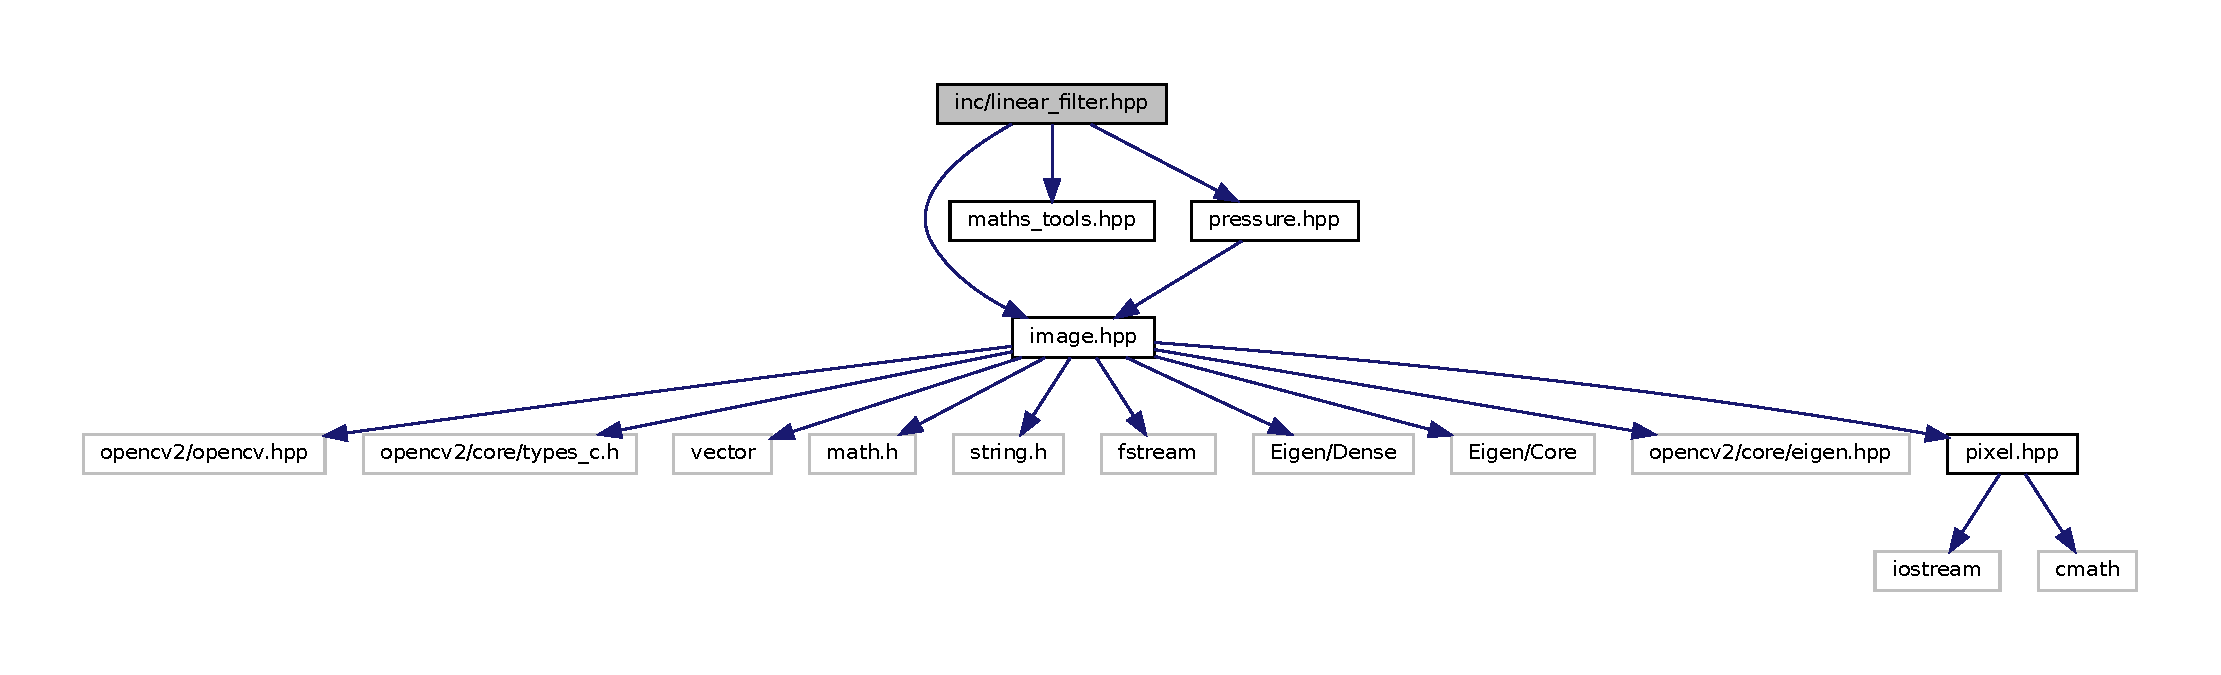
\includegraphics[width=350pt]{linear__filter_8hpp__incl}
\end{center}
\end{figure}
This graph shows which files directly or indirectly include this file\+:
\nopagebreak
\begin{figure}[H]
\begin{center}
\leavevmode
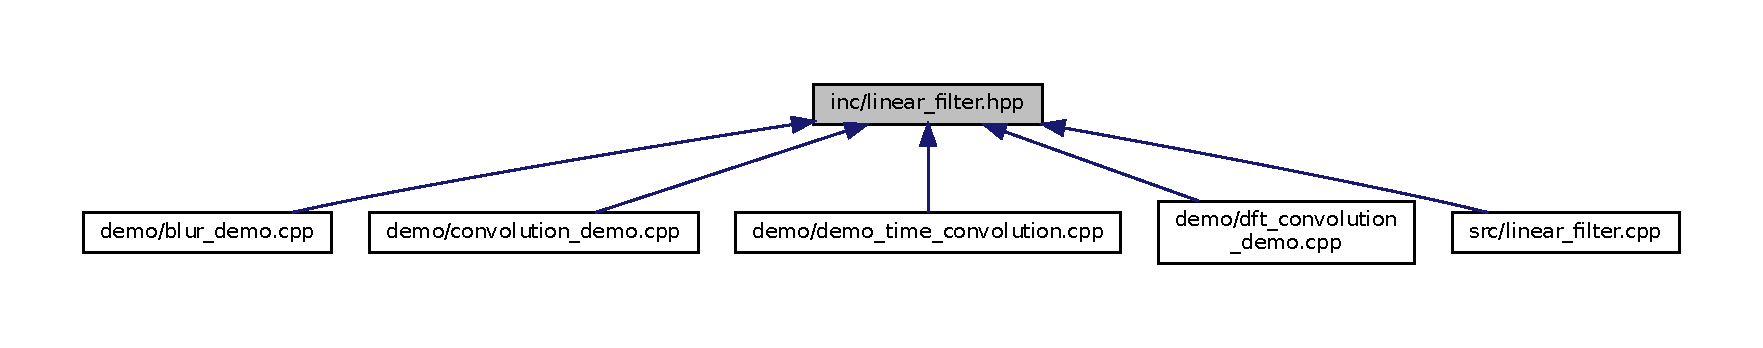
\includegraphics[width=350pt]{linear__filter_8hpp__dep__incl}
\end{center}
\end{figure}
\subsection*{Functions}
\begin{DoxyCompactItemize}
\item 
void \hyperlink{linear__filter_8hpp_ad1b837554f9911e4bf91c60bd43b5df2}{shift} (cv\+::\+Mat magI)
\begin{DoxyCompactList}\small\item\em \+: Shift subparts of input $\ast$ \end{DoxyCompactList}\item 
cv\+::\+Mat \hyperlink{linear__filter_8hpp_a1c9c777c748a21c0e0d4537dbd0e9bae}{update\+Mag} (cv\+::\+Mat complex)
\begin{DoxyCompactList}\small\item\em \+: Compute the matrix of magnitude $\ast$ \end{DoxyCompactList}\item 
cv\+::\+Mat \hyperlink{linear__filter_8hpp_a86bade9e2cd4aa9230fc6d8e3833b147}{create\+Filter\+Mask} (cv\+::\+Size imsize, const cv\+::\+Mat \&kernelX, const cv\+::\+Mat \&kernelY)
\begin{DoxyCompactList}\small\item\em Create a mask (or kernel) by matricial multiplication between two vectors. The sum of the two vectors should equal 1 to preserve the energy by convolution. \end{DoxyCompactList}\item 
float \hyperlink{linear__filter_8hpp_adc05d0d856da04e78bbde8b311f17203}{search\+\_\+max} (const cv\+::\+Mat \&image)
\begin{DoxyCompactList}\small\item\em \+: Returns the maximum intensity present in the Matrix \end{DoxyCompactList}\item 
std\+::vector$<$ float $>$ \hyperlink{linear__filter_8hpp_afe688b7431925c587389dc73cc42180a}{Mat\+\_\+to\+\_\+vector} (const cv\+::\+Mat \&matrix)
\end{DoxyCompactItemize}


\subsection{Function Documentation}
\mbox{\Hypertarget{linear__filter_8hpp_a86bade9e2cd4aa9230fc6d8e3833b147}\label{linear__filter_8hpp_a86bade9e2cd4aa9230fc6d8e3833b147}} 
\index{linear\+\_\+filter.\+hpp@{linear\+\_\+filter.\+hpp}!create\+Filter\+Mask@{create\+Filter\+Mask}}
\index{create\+Filter\+Mask@{create\+Filter\+Mask}!linear\+\_\+filter.\+hpp@{linear\+\_\+filter.\+hpp}}
\subsubsection{\texorpdfstring{create\+Filter\+Mask()}{createFilterMask()}}
{\footnotesize\ttfamily cv\+::\+Mat create\+Filter\+Mask (\begin{DoxyParamCaption}\item[{cv\+::\+Size}]{imsize,  }\item[{const cv\+::\+Mat \&}]{kernelX,  }\item[{const cv\+::\+Mat \&}]{kernelY }\end{DoxyParamCaption})}



Create a mask (or kernel) by matricial multiplication between two vectors. The sum of the two vectors should equal 1 to preserve the energy by convolution. 


\begin{DoxyParams}{Parameters}
{\em imsize} & \+: Size of the output Matrix \\
\hline
{\em kernelX} & \+: Must be a column vector. \\
\hline
{\em kernelY} & \+: Must be a column vector. \\
\hline
\end{DoxyParams}
\begin{DoxyReturn}{Returns}
\+: Matrix of the kernel. The kernel is placed in the middle of the matrix. The, to complete the size, we pad the matrix with zeros around the kernel. 
\end{DoxyReturn}
\mbox{\Hypertarget{linear__filter_8hpp_afe688b7431925c587389dc73cc42180a}\label{linear__filter_8hpp_afe688b7431925c587389dc73cc42180a}} 
\index{linear\+\_\+filter.\+hpp@{linear\+\_\+filter.\+hpp}!Mat\+\_\+to\+\_\+vector@{Mat\+\_\+to\+\_\+vector}}
\index{Mat\+\_\+to\+\_\+vector@{Mat\+\_\+to\+\_\+vector}!linear\+\_\+filter.\+hpp@{linear\+\_\+filter.\+hpp}}
\subsubsection{\texorpdfstring{Mat\+\_\+to\+\_\+vector()}{Mat\_to\_vector()}}
{\footnotesize\ttfamily std\+::vector$<$float$>$ Mat\+\_\+to\+\_\+vector (\begin{DoxyParamCaption}\item[{const cv\+::\+Mat \&}]{matrix }\end{DoxyParamCaption})}

Convert a mat object in a vector type \mbox{\Hypertarget{linear__filter_8hpp_adc05d0d856da04e78bbde8b311f17203}\label{linear__filter_8hpp_adc05d0d856da04e78bbde8b311f17203}} 
\index{linear\+\_\+filter.\+hpp@{linear\+\_\+filter.\+hpp}!search\+\_\+max@{search\+\_\+max}}
\index{search\+\_\+max@{search\+\_\+max}!linear\+\_\+filter.\+hpp@{linear\+\_\+filter.\+hpp}}
\subsubsection{\texorpdfstring{search\+\_\+max()}{search\_max()}}
{\footnotesize\ttfamily float search\+\_\+max (\begin{DoxyParamCaption}\item[{const cv\+::\+Mat \&}]{image }\end{DoxyParamCaption})}



\+: Returns the maximum intensity present in the Matrix 

\mbox{\Hypertarget{linear__filter_8hpp_ad1b837554f9911e4bf91c60bd43b5df2}\label{linear__filter_8hpp_ad1b837554f9911e4bf91c60bd43b5df2}} 
\index{linear\+\_\+filter.\+hpp@{linear\+\_\+filter.\+hpp}!shift@{shift}}
\index{shift@{shift}!linear\+\_\+filter.\+hpp@{linear\+\_\+filter.\+hpp}}
\subsubsection{\texorpdfstring{shift()}{shift()}}
{\footnotesize\ttfamily void shift (\begin{DoxyParamCaption}\item[{cv\+::\+Mat}]{magI }\end{DoxyParamCaption})}



\+: Shift subparts of input $\ast$ 


\begin{DoxyParams}{Parameters}
{\em magI} & \+: \hyperlink{class_image}{Image} to be shifted \\
\hline
\end{DoxyParams}
\mbox{\Hypertarget{linear__filter_8hpp_a1c9c777c748a21c0e0d4537dbd0e9bae}\label{linear__filter_8hpp_a1c9c777c748a21c0e0d4537dbd0e9bae}} 
\index{linear\+\_\+filter.\+hpp@{linear\+\_\+filter.\+hpp}!update\+Mag@{update\+Mag}}
\index{update\+Mag@{update\+Mag}!linear\+\_\+filter.\+hpp@{linear\+\_\+filter.\+hpp}}
\subsubsection{\texorpdfstring{update\+Mag()}{updateMag()}}
{\footnotesize\ttfamily cv\+::\+Mat update\+Mag (\begin{DoxyParamCaption}\item[{cv\+::\+Mat}]{complex }\end{DoxyParamCaption})}



\+: Compute the matrix of magnitude $\ast$ 


\begin{DoxyParams}{Parameters}
{\em complex} & \+: Matrix under complex form $\ast$ \\
\hline
\end{DoxyParams}
\begin{DoxyReturn}{Returns}
Matrix of magnitudes 
\end{DoxyReturn}

\hypertarget{maths__tools_8hpp}{}\section{inc/maths\+\_\+tools.hpp File Reference}
\label{maths__tools_8hpp}\index{inc/maths\+\_\+tools.\+hpp@{inc/maths\+\_\+tools.\+hpp}}
This graph shows which files directly or indirectly include this file\+:
\nopagebreak
\begin{figure}[H]
\begin{center}
\leavevmode
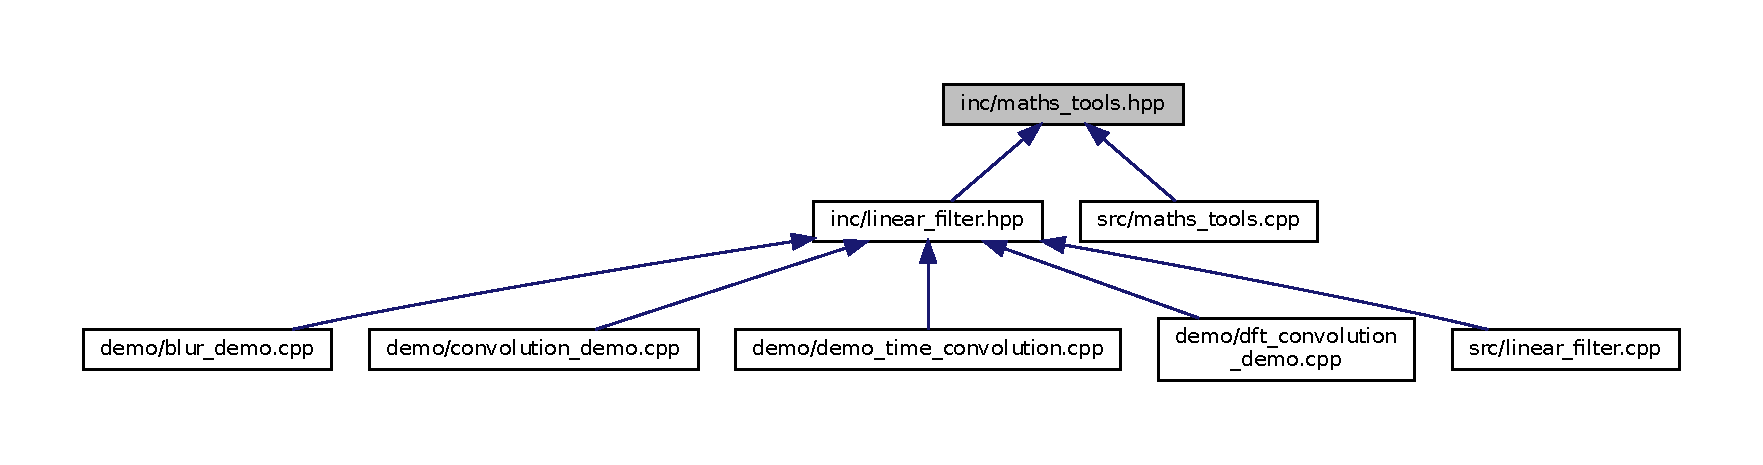
\includegraphics[width=350pt]{maths__tools_8hpp__dep__incl}
\end{center}
\end{figure}
\subsection*{Functions}
\begin{DoxyCompactItemize}
\item 
bool \hyperlink{maths__tools_8hpp_a1e001dd81543d53ce05eef3b6dc4a7a3}{between} (int r, int a, int b)
\begin{DoxyCompactList}\small\item\em \+: Return true if r is between a and b. \end{DoxyCompactList}\end{DoxyCompactItemize}


\subsection{Function Documentation}
\mbox{\Hypertarget{maths__tools_8hpp_a1e001dd81543d53ce05eef3b6dc4a7a3}\label{maths__tools_8hpp_a1e001dd81543d53ce05eef3b6dc4a7a3}} 
\index{maths\+\_\+tools.\+hpp@{maths\+\_\+tools.\+hpp}!between@{between}}
\index{between@{between}!maths\+\_\+tools.\+hpp@{maths\+\_\+tools.\+hpp}}
\subsubsection{\texorpdfstring{between()}{between()}}
{\footnotesize\ttfamily bool between (\begin{DoxyParamCaption}\item[{int}]{r,  }\item[{int}]{a,  }\item[{int}]{b }\end{DoxyParamCaption})}



\+: Return true if r is between a and b. 


\hypertarget{optimization_8hpp}{}\section{inc/optimization.hpp File Reference}
\label{optimization_8hpp}\index{inc/optimization.\+hpp@{inc/optimization.\+hpp}}
{\ttfamily \#include \char`\"{}image.\+hpp\char`\"{}}\newline
{\ttfamily \#include $<$assert.\+h$>$}\newline
Include dependency graph for optimization.\+hpp\+:
\nopagebreak
\begin{figure}[H]
\begin{center}
\leavevmode
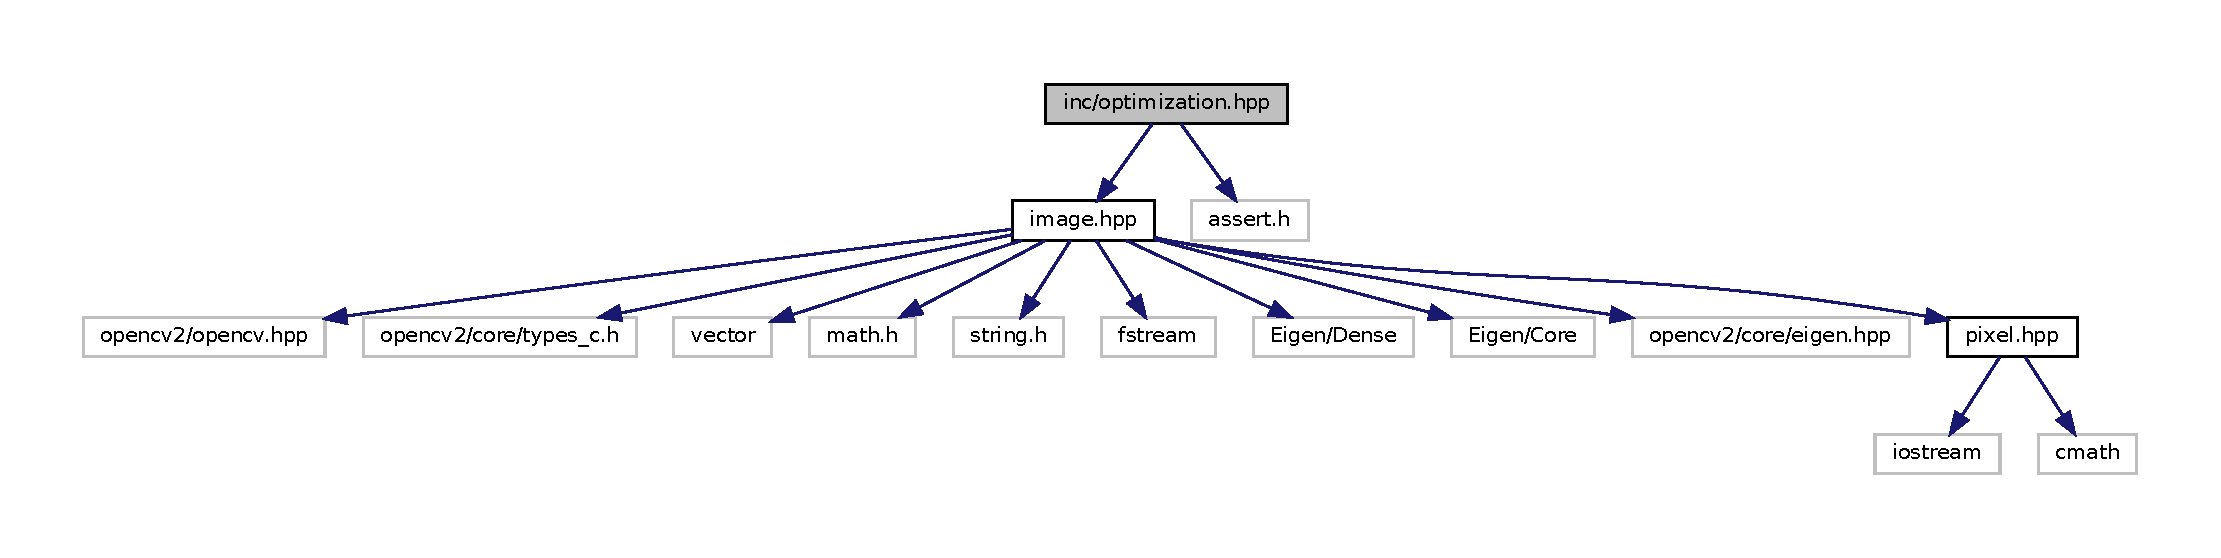
\includegraphics[width=350pt]{optimization_8hpp__incl}
\end{center}
\end{figure}
This graph shows which files directly or indirectly include this file\+:
\nopagebreak
\begin{figure}[H]
\begin{center}
\leavevmode
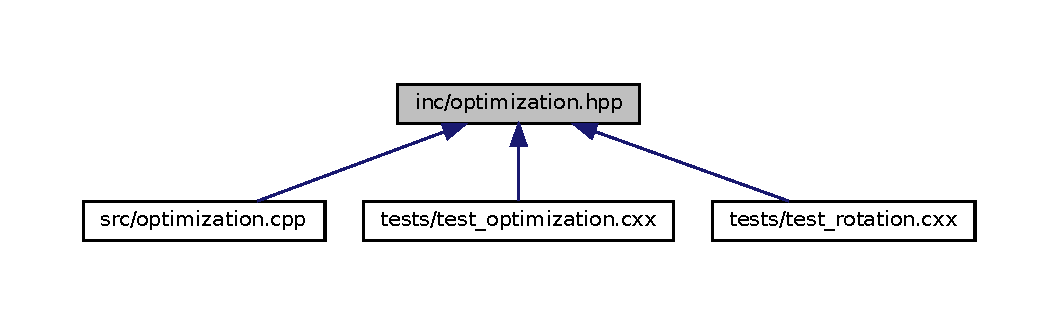
\includegraphics[width=350pt]{optimization_8hpp__dep__incl}
\end{center}
\end{figure}
\subsection*{Functions}
\begin{DoxyCompactItemize}
\item 
int \hyperlink{optimization_8hpp_a9ee1e4e7beea5a472fe21ed2bd97ddf2}{optimize} (std\+::vector$<$ float $>$ list\+\_\+l, bool max)
\begin{DoxyCompactList}\small\item\em Find the index of the maximum or the minimum (correlation or squared error) of the values of loss function in the vector. \end{DoxyCompactList}\item 
bool \hyperlink{optimization_8hpp_a532ed4571db526e7215785ece8d31efe}{equal\+\_\+vector} (std\+::vector$<$ float $>$ \&v, std\+::vector$<$ float $>$ \&w)
\begin{DoxyCompactList}\small\item\em Function which return true if the two vectors are equals down to 0.\+001, false otherwise. \end{DoxyCompactList}\item 
void \hyperlink{optimization_8hpp_a781986c541a7394e5c2f86e29643fb0d}{copy\+\_\+tab3} (float tab1\mbox{[}3\mbox{]}, float tab2\mbox{[}4\mbox{]})
\begin{DoxyCompactList}\small\item\em Made a copy of a table of size 3 in an other. \end{DoxyCompactList}\end{DoxyCompactItemize}


\subsection{Function Documentation}
\mbox{\Hypertarget{optimization_8hpp_a781986c541a7394e5c2f86e29643fb0d}\label{optimization_8hpp_a781986c541a7394e5c2f86e29643fb0d}} 
\index{optimization.\+hpp@{optimization.\+hpp}!copy\+\_\+tab3@{copy\+\_\+tab3}}
\index{copy\+\_\+tab3@{copy\+\_\+tab3}!optimization.\+hpp@{optimization.\+hpp}}
\subsubsection{\texorpdfstring{copy\+\_\+tab3()}{copy\_tab3()}}
{\footnotesize\ttfamily void copy\+\_\+tab3 (\begin{DoxyParamCaption}\item[{float}]{tab1\mbox{[}3\mbox{]},  }\item[{float}]{tab2\mbox{[}4\mbox{]} }\end{DoxyParamCaption})}



Made a copy of a table of size 3 in an other. 


\begin{DoxyParams}{Parameters}
{\em two} & tables of size 3. \\
\hline
\end{DoxyParams}
\mbox{\Hypertarget{optimization_8hpp_a532ed4571db526e7215785ece8d31efe}\label{optimization_8hpp_a532ed4571db526e7215785ece8d31efe}} 
\index{optimization.\+hpp@{optimization.\+hpp}!equal\+\_\+vector@{equal\+\_\+vector}}
\index{equal\+\_\+vector@{equal\+\_\+vector}!optimization.\+hpp@{optimization.\+hpp}}
\subsubsection{\texorpdfstring{equal\+\_\+vector()}{equal\_vector()}}
{\footnotesize\ttfamily bool equal\+\_\+vector (\begin{DoxyParamCaption}\item[{std\+::vector$<$ float $>$ \&}]{v,  }\item[{std\+::vector$<$ float $>$ \&}]{w }\end{DoxyParamCaption})}



Function which return true if the two vectors are equals down to 0.\+001, false otherwise. 


\begin{DoxyParams}{Parameters}
{\em two} & vectors of floats \\
\hline
\end{DoxyParams}
\mbox{\Hypertarget{optimization_8hpp_a9ee1e4e7beea5a472fe21ed2bd97ddf2}\label{optimization_8hpp_a9ee1e4e7beea5a472fe21ed2bd97ddf2}} 
\index{optimization.\+hpp@{optimization.\+hpp}!optimize@{optimize}}
\index{optimize@{optimize}!optimization.\+hpp@{optimization.\+hpp}}
\subsubsection{\texorpdfstring{optimize()}{optimize()}}
{\footnotesize\ttfamily int optimize (\begin{DoxyParamCaption}\item[{std\+::vector$<$ float $>$}]{list\+\_\+l,  }\item[{bool}]{squared }\end{DoxyParamCaption})}



Find the index of the maximum or the minimum (correlation or squared error) of the values of loss function in the vector. 


\begin{DoxyParams}{Parameters}
{\em a} & vector of the loss function values for a set of images, a boolean which is true if the loss function used is the squared error, false if it\textquotesingle{}s the correlation. \\
\hline
\end{DoxyParams}
\begin{DoxyReturn}{Returns}
the index of the optimized value in the vector 
\end{DoxyReturn}

\hypertarget{pixel_8hpp}{}\section{inc/pixel.hpp File Reference}
\label{pixel_8hpp}\index{inc/pixel.\+hpp@{inc/pixel.\+hpp}}
{\ttfamily \#include $<$iostream$>$}\newline
{\ttfamily \#include $<$cmath$>$}\newline
Include dependency graph for pixel.\+hpp\+:
\nopagebreak
\begin{figure}[H]
\begin{center}
\leavevmode
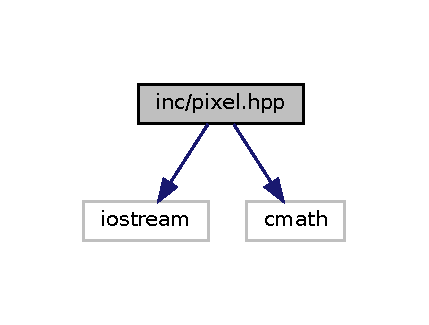
\includegraphics[width=206pt]{pixel_8hpp__incl}
\end{center}
\end{figure}
This graph shows which files directly or indirectly include this file\+:
\nopagebreak
\begin{figure}[H]
\begin{center}
\leavevmode
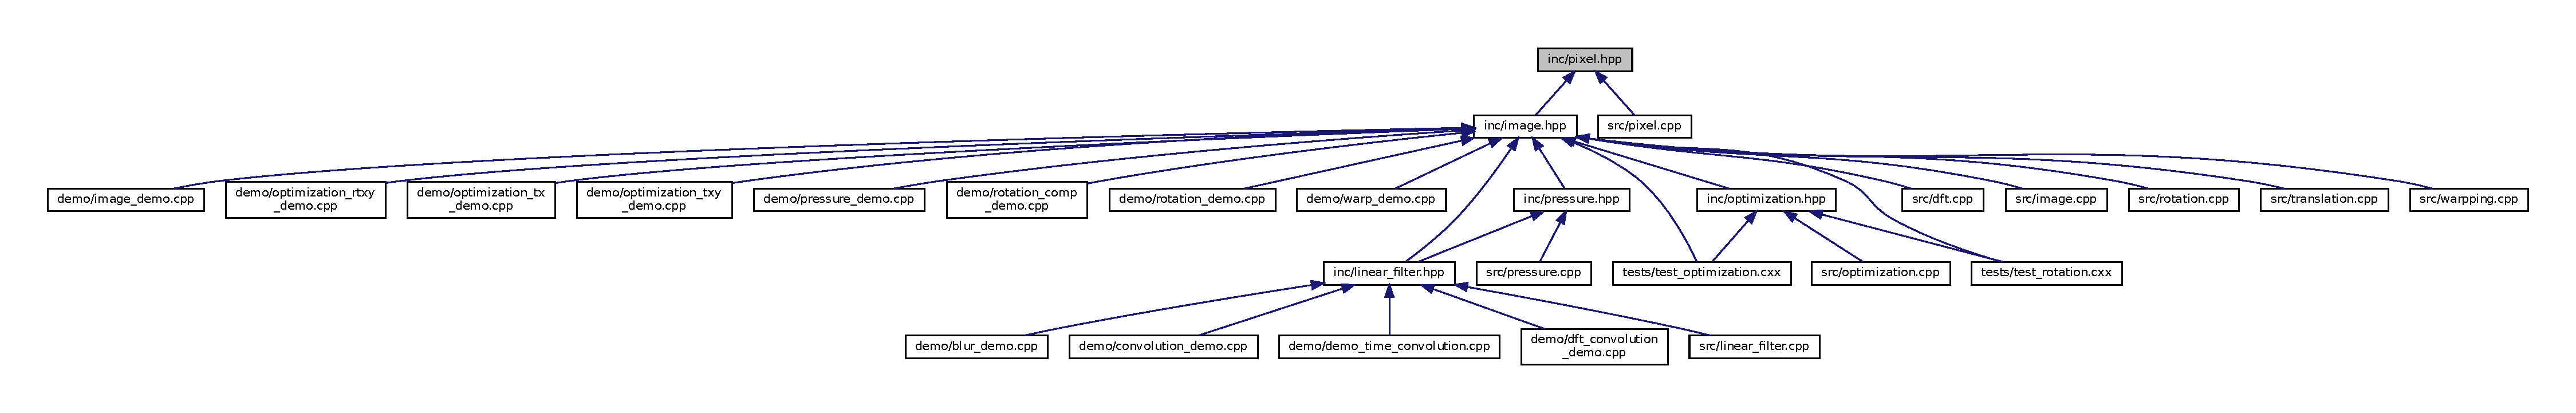
\includegraphics[width=350pt]{pixel_8hpp__dep__incl}
\end{center}
\end{figure}
\subsection*{Classes}
\begin{DoxyCompactItemize}
\item 
class \hyperlink{class_pixel}{Pixel}
\end{DoxyCompactItemize}

\hypertarget{pressure_8hpp}{}\section{inc/pressure.hpp File Reference}
\label{pressure_8hpp}\index{inc/pressure.\+hpp@{inc/pressure.\+hpp}}
{\ttfamily \#include \char`\"{}image.\+hpp\char`\"{}}\newline
Include dependency graph for pressure.\+hpp\+:
\nopagebreak
\begin{figure}[H]
\begin{center}
\leavevmode
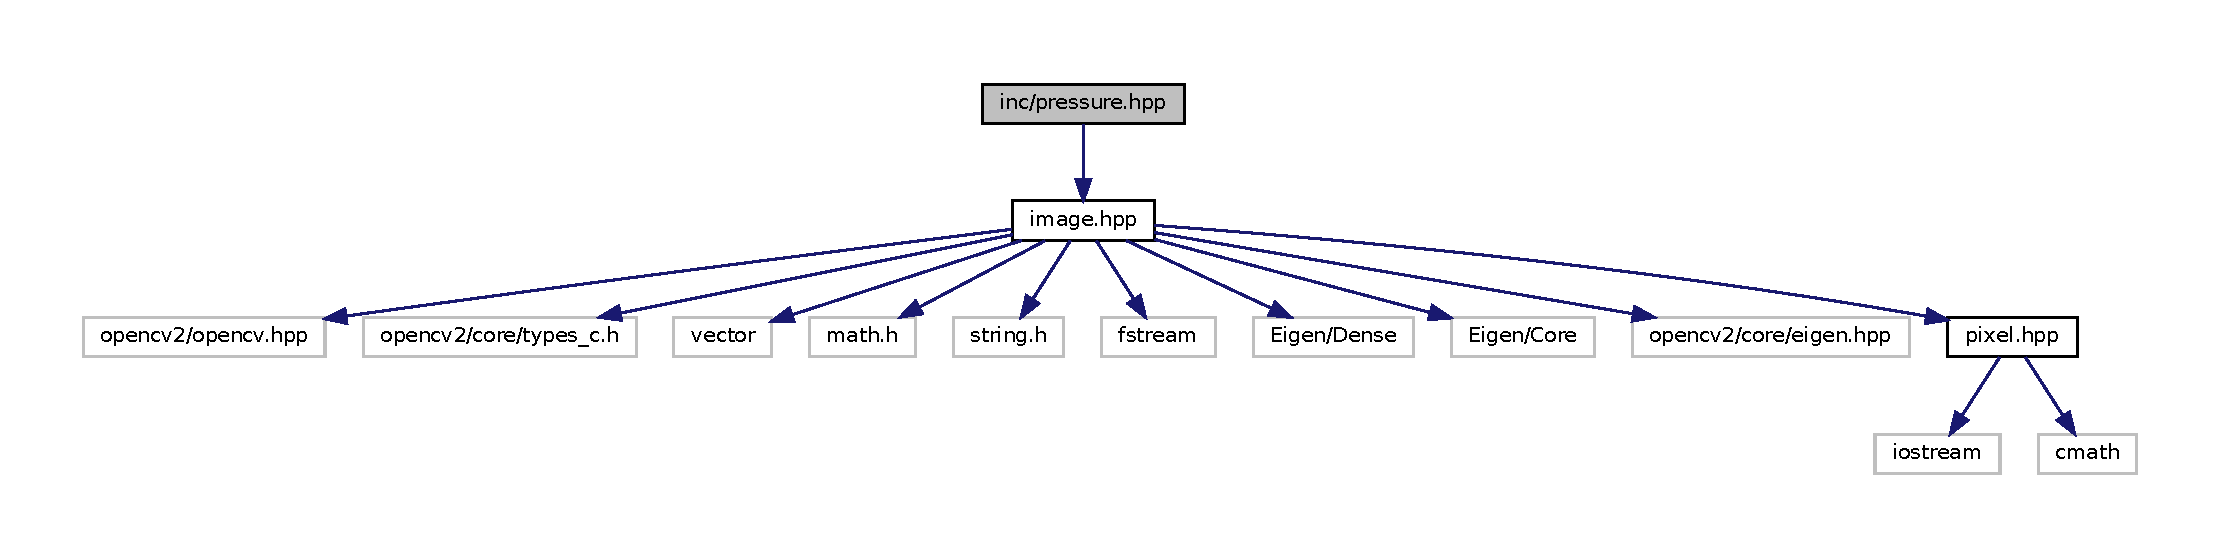
\includegraphics[width=350pt]{pressure_8hpp__incl}
\end{center}
\end{figure}
This graph shows which files directly or indirectly include this file\+:
\nopagebreak
\begin{figure}[H]
\begin{center}
\leavevmode
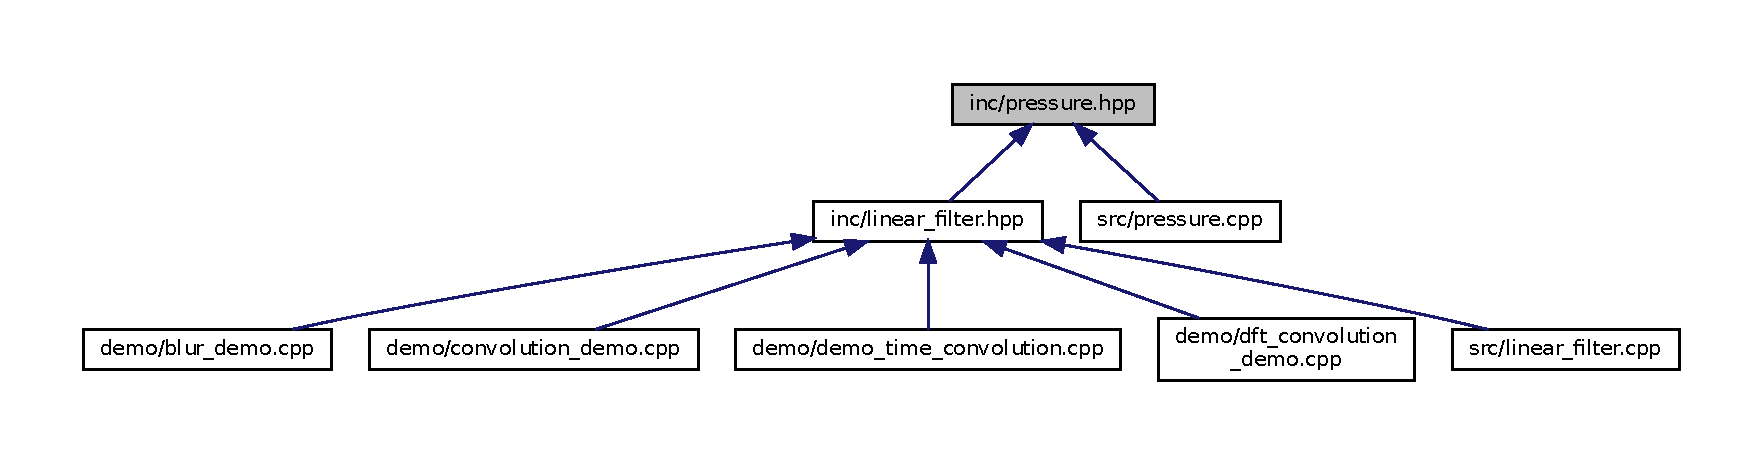
\includegraphics[width=350pt]{pressure_8hpp__dep__incl}
\end{center}
\end{figure}
\subsection*{Functions}
\begin{DoxyCompactItemize}
\item 
float \hyperlink{pressure_8hpp_a44fb8b67c9a0fb92ac38e1c5d3cae7cd}{weight\+\_\+exp} (float coeff, int power, float r)
\begin{DoxyCompactList}\small\item\em Exponential attenuation function. \end{DoxyCompactList}\end{DoxyCompactItemize}


\subsection{Function Documentation}
\mbox{\Hypertarget{pressure_8hpp_a44fb8b67c9a0fb92ac38e1c5d3cae7cd}\label{pressure_8hpp_a44fb8b67c9a0fb92ac38e1c5d3cae7cd}} 
\index{pressure.\+hpp@{pressure.\+hpp}!weight\+\_\+exp@{weight\+\_\+exp}}
\index{weight\+\_\+exp@{weight\+\_\+exp}!pressure.\+hpp@{pressure.\+hpp}}
\subsubsection{\texorpdfstring{weight\+\_\+exp()}{weight\_exp()}}
{\footnotesize\ttfamily float weight\+\_\+exp (\begin{DoxyParamCaption}\item[{float}]{coeff,  }\item[{int}]{power,  }\item[{float}]{r }\end{DoxyParamCaption})}



Exponential attenuation function. 


\begin{DoxyParams}{Parameters}
{\em \hyperlink{class_image}{Image}} & \+: float \+: coefficient of attenuation, int \+: power, float \+: parameter. \\
\hline
\end{DoxyParams}

\hypertarget{_r_e_a_d_m_e_8md}{}\section{R\+E\+A\+D\+M\+E.\+md File Reference}
\label{_r_e_a_d_m_e_8md}\index{R\+E\+A\+D\+M\+E.\+md@{R\+E\+A\+D\+M\+E.\+md}}

\hypertarget{dft_8cpp}{}\section{src/dft.cpp File Reference}
\label{dft_8cpp}\index{src/dft.\+cpp@{src/dft.\+cpp}}
{\ttfamily \#include \char`\"{}image.\+hpp\char`\"{}}\newline
Include dependency graph for dft.\+cpp\+:
\nopagebreak
\begin{figure}[H]
\begin{center}
\leavevmode
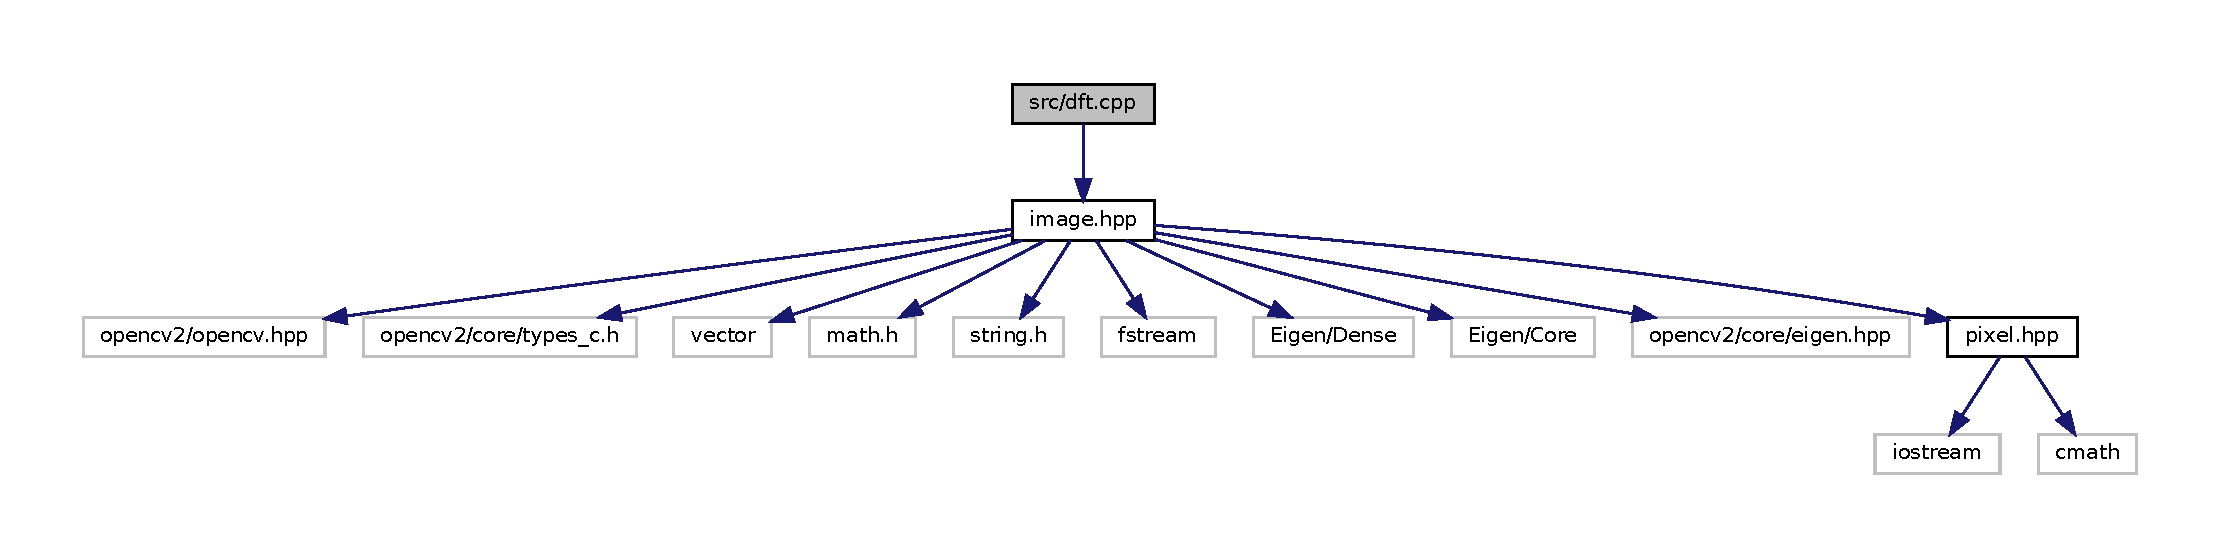
\includegraphics[width=350pt]{dft_8cpp__incl}
\end{center}
\end{figure}

\hypertarget{image_8cpp}{}\section{src/image.cpp File Reference}
\label{image_8cpp}\index{src/image.\+cpp@{src/image.\+cpp}}


Definition of image class methods.  


{\ttfamily \#include \char`\"{}image.\+hpp\char`\"{}}\newline
Include dependency graph for image.\+cpp\+:
\nopagebreak
\begin{figure}[H]
\begin{center}
\leavevmode
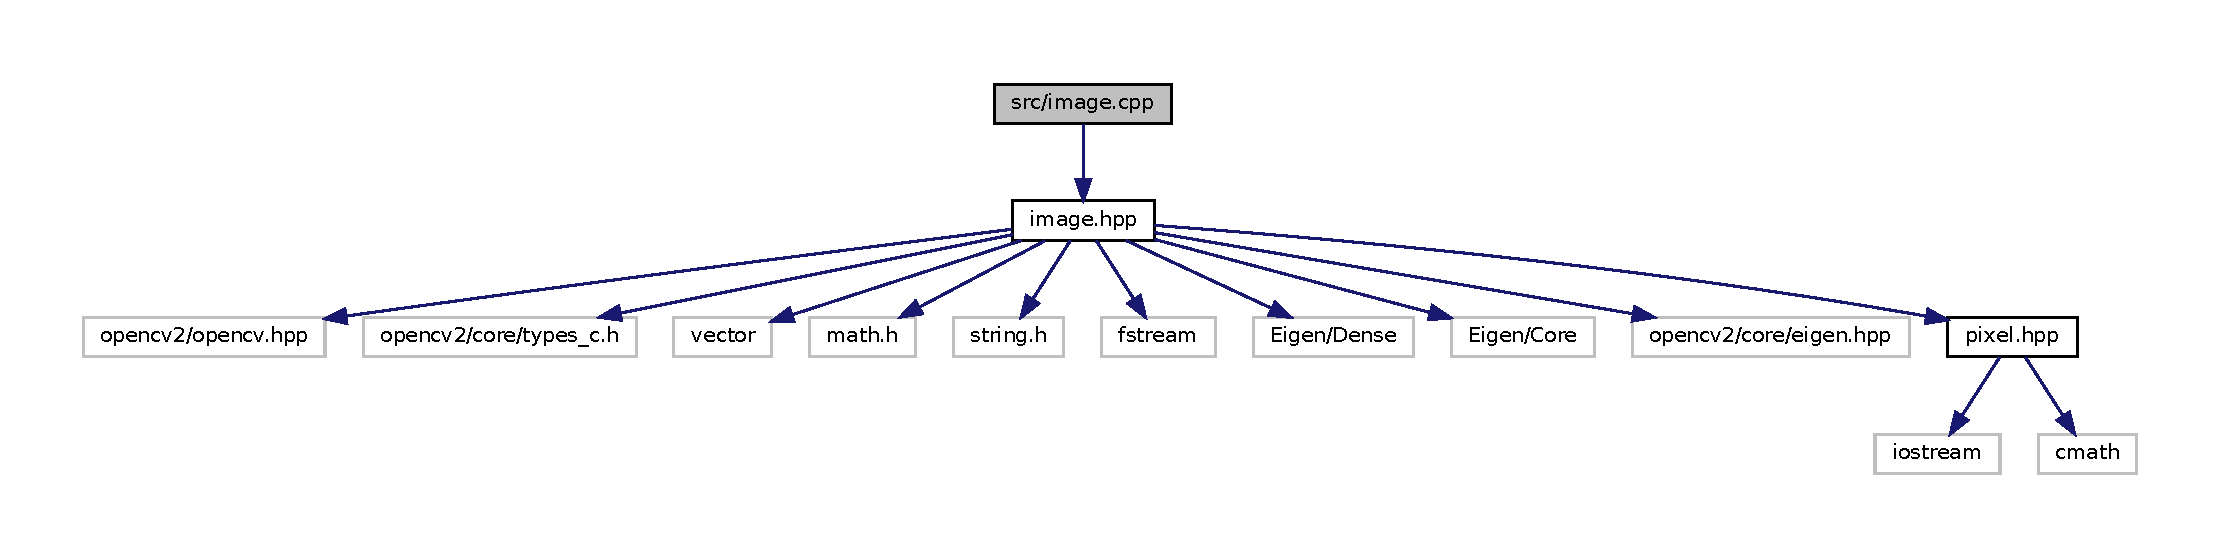
\includegraphics[width=350pt]{image_8cpp__incl}
\end{center}
\end{figure}


\subsection{Detailed Description}
Definition of image class methods. 

\begin{DoxyAuthor}{Author}
Perrine, Célestine, Aurélien, Lucas 
\end{DoxyAuthor}
\begin{DoxyDate}{Date}
01/08/2019 
\end{DoxyDate}

\hypertarget{linear__filter_8cpp}{}\section{src/linear\+\_\+filter.cpp File Reference}
\label{linear__filter_8cpp}\index{src/linear\+\_\+filter.\+cpp@{src/linear\+\_\+filter.\+cpp}}


Definition of methods concerning the linear filtering.  


{\ttfamily \#include \char`\"{}linear\+\_\+filter.\+hpp\char`\"{}}\newline
Include dependency graph for linear\+\_\+filter.\+cpp\+:
\nopagebreak
\begin{figure}[H]
\begin{center}
\leavevmode
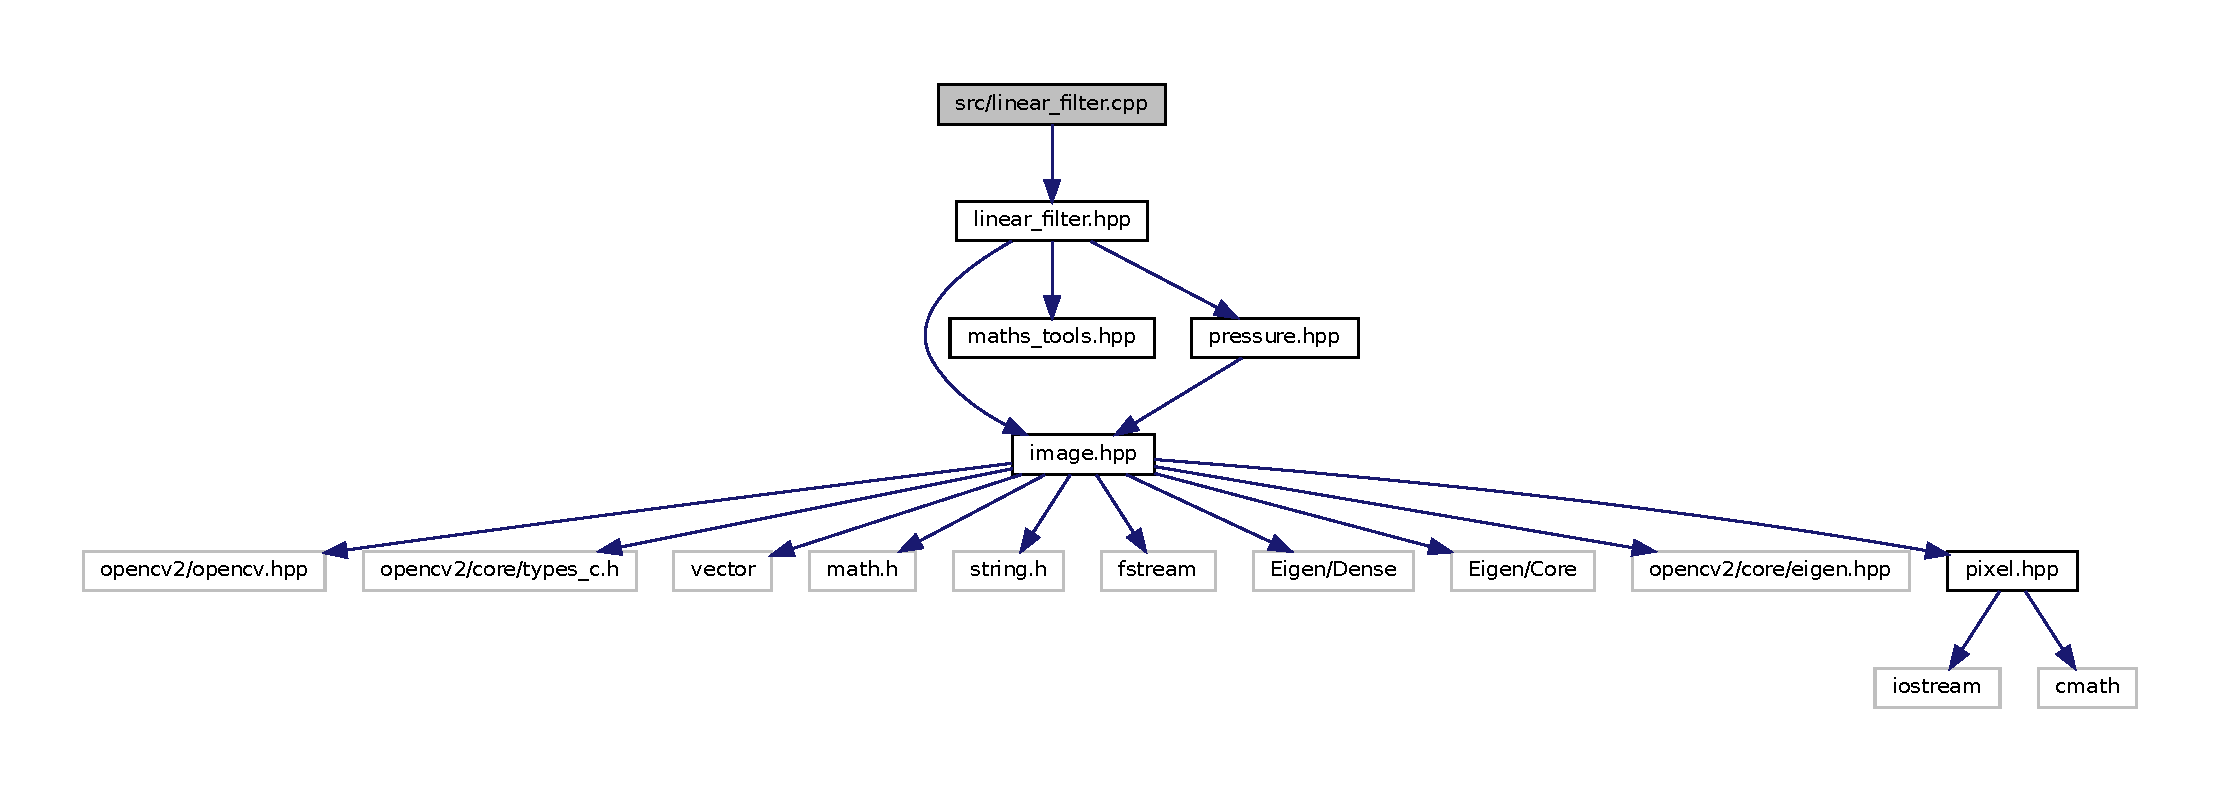
\includegraphics[width=350pt]{linear__filter_8cpp__incl}
\end{center}
\end{figure}
\subsection*{Functions}
\begin{DoxyCompactItemize}
\item 
void \hyperlink{linear__filter_8cpp_a856caac33d6b5cf718f168e8a14aaed3}{shift} (Mat magI)
\item 
Mat \hyperlink{linear__filter_8cpp_a450e66dbcac8bcfbb551c88196e96529}{update\+Mag} (Mat complex)
\item 
Mat \hyperlink{linear__filter_8cpp_a7da1ca57ead7bbf0d2ce4432bd3a72f0}{create\+Filter\+Mask} (Size imsize, const Mat \&kernelX, const Mat \&kernelY)
\item 
std\+::vector$<$ float $>$ \hyperlink{linear__filter_8cpp_ab0856ea1389c695cc6a92d52dd655007}{Mat\+\_\+to\+\_\+vector} (const Mat \&matrix)
\end{DoxyCompactItemize}


\subsection{Detailed Description}
Definition of methods concerning the linear filtering. 

Implementation of functions used for 2D convolution.

\begin{DoxyAuthor}{Author}
Perrine, Célestine, Aurélien, Lucas 
\end{DoxyAuthor}
\begin{DoxyDate}{Date}
01/21/2019
\end{DoxyDate}
\begin{DoxyAuthor}{Author}
Perrine, Célestine, Aurélien, Lucas 
\end{DoxyAuthor}
\begin{DoxyDate}{Date}
19.\+01.\+2019 
\end{DoxyDate}


\subsection{Function Documentation}
\mbox{\Hypertarget{linear__filter_8cpp_a7da1ca57ead7bbf0d2ce4432bd3a72f0}\label{linear__filter_8cpp_a7da1ca57ead7bbf0d2ce4432bd3a72f0}} 
\index{linear\+\_\+filter.\+cpp@{linear\+\_\+filter.\+cpp}!create\+Filter\+Mask@{create\+Filter\+Mask}}
\index{create\+Filter\+Mask@{create\+Filter\+Mask}!linear\+\_\+filter.\+cpp@{linear\+\_\+filter.\+cpp}}
\subsubsection{\texorpdfstring{create\+Filter\+Mask()}{createFilterMask()}}
{\footnotesize\ttfamily Mat create\+Filter\+Mask (\begin{DoxyParamCaption}\item[{Size}]{imsize,  }\item[{const Mat \&}]{kernelX,  }\item[{const Mat \&}]{kernelY }\end{DoxyParamCaption})}

\mbox{\Hypertarget{linear__filter_8cpp_ab0856ea1389c695cc6a92d52dd655007}\label{linear__filter_8cpp_ab0856ea1389c695cc6a92d52dd655007}} 
\index{linear\+\_\+filter.\+cpp@{linear\+\_\+filter.\+cpp}!Mat\+\_\+to\+\_\+vector@{Mat\+\_\+to\+\_\+vector}}
\index{Mat\+\_\+to\+\_\+vector@{Mat\+\_\+to\+\_\+vector}!linear\+\_\+filter.\+cpp@{linear\+\_\+filter.\+cpp}}
\subsubsection{\texorpdfstring{Mat\+\_\+to\+\_\+vector()}{Mat\_to\_vector()}}
{\footnotesize\ttfamily std\+::vector$<$float$>$ Mat\+\_\+to\+\_\+vector (\begin{DoxyParamCaption}\item[{const Mat \&}]{matrix }\end{DoxyParamCaption})}

\mbox{\Hypertarget{linear__filter_8cpp_a856caac33d6b5cf718f168e8a14aaed3}\label{linear__filter_8cpp_a856caac33d6b5cf718f168e8a14aaed3}} 
\index{linear\+\_\+filter.\+cpp@{linear\+\_\+filter.\+cpp}!shift@{shift}}
\index{shift@{shift}!linear\+\_\+filter.\+cpp@{linear\+\_\+filter.\+cpp}}
\subsubsection{\texorpdfstring{shift()}{shift()}}
{\footnotesize\ttfamily void shift (\begin{DoxyParamCaption}\item[{Mat}]{magI }\end{DoxyParamCaption})}

\mbox{\Hypertarget{linear__filter_8cpp_a450e66dbcac8bcfbb551c88196e96529}\label{linear__filter_8cpp_a450e66dbcac8bcfbb551c88196e96529}} 
\index{linear\+\_\+filter.\+cpp@{linear\+\_\+filter.\+cpp}!update\+Mag@{update\+Mag}}
\index{update\+Mag@{update\+Mag}!linear\+\_\+filter.\+cpp@{linear\+\_\+filter.\+cpp}}
\subsubsection{\texorpdfstring{update\+Mag()}{updateMag()}}
{\footnotesize\ttfamily Mat update\+Mag (\begin{DoxyParamCaption}\item[{Mat}]{complex }\end{DoxyParamCaption})}


\hypertarget{maths__tools_8cpp}{}\section{src/maths\+\_\+tools.cpp File Reference}
\label{maths__tools_8cpp}\index{src/maths\+\_\+tools.\+cpp@{src/maths\+\_\+tools.\+cpp}}
{\ttfamily \#include \char`\"{}maths\+\_\+tools.\+hpp\char`\"{}}\newline
Include dependency graph for maths\+\_\+tools.\+cpp\+:
\nopagebreak
\begin{figure}[H]
\begin{center}
\leavevmode
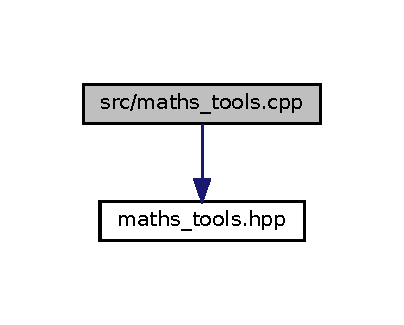
\includegraphics[width=194pt]{maths__tools_8cpp__incl}
\end{center}
\end{figure}
\subsection*{Functions}
\begin{DoxyCompactItemize}
\item 
bool \hyperlink{maths__tools_8cpp_a1e001dd81543d53ce05eef3b6dc4a7a3}{between} (int r, int a, int b)
\begin{DoxyCompactList}\small\item\em \+: Return true if r is between a and b. \end{DoxyCompactList}\end{DoxyCompactItemize}


\subsection{Function Documentation}
\mbox{\Hypertarget{maths__tools_8cpp_a1e001dd81543d53ce05eef3b6dc4a7a3}\label{maths__tools_8cpp_a1e001dd81543d53ce05eef3b6dc4a7a3}} 
\index{maths\+\_\+tools.\+cpp@{maths\+\_\+tools.\+cpp}!between@{between}}
\index{between@{between}!maths\+\_\+tools.\+cpp@{maths\+\_\+tools.\+cpp}}
\subsubsection{\texorpdfstring{between()}{between()}}
{\footnotesize\ttfamily bool between (\begin{DoxyParamCaption}\item[{int}]{r,  }\item[{int}]{a,  }\item[{int}]{b }\end{DoxyParamCaption})}



\+: Return true if r is between a and b. 


\hypertarget{optimization_8cpp}{}\section{src/optimization.cpp File Reference}
\label{optimization_8cpp}\index{src/optimization.\+cpp@{src/optimization.\+cpp}}


Set of optimization methods and function.  


{\ttfamily \#include \char`\"{}optimization.\+hpp\char`\"{}}\newline
Include dependency graph for optimization.\+cpp\+:
\nopagebreak
\begin{figure}[H]
\begin{center}
\leavevmode
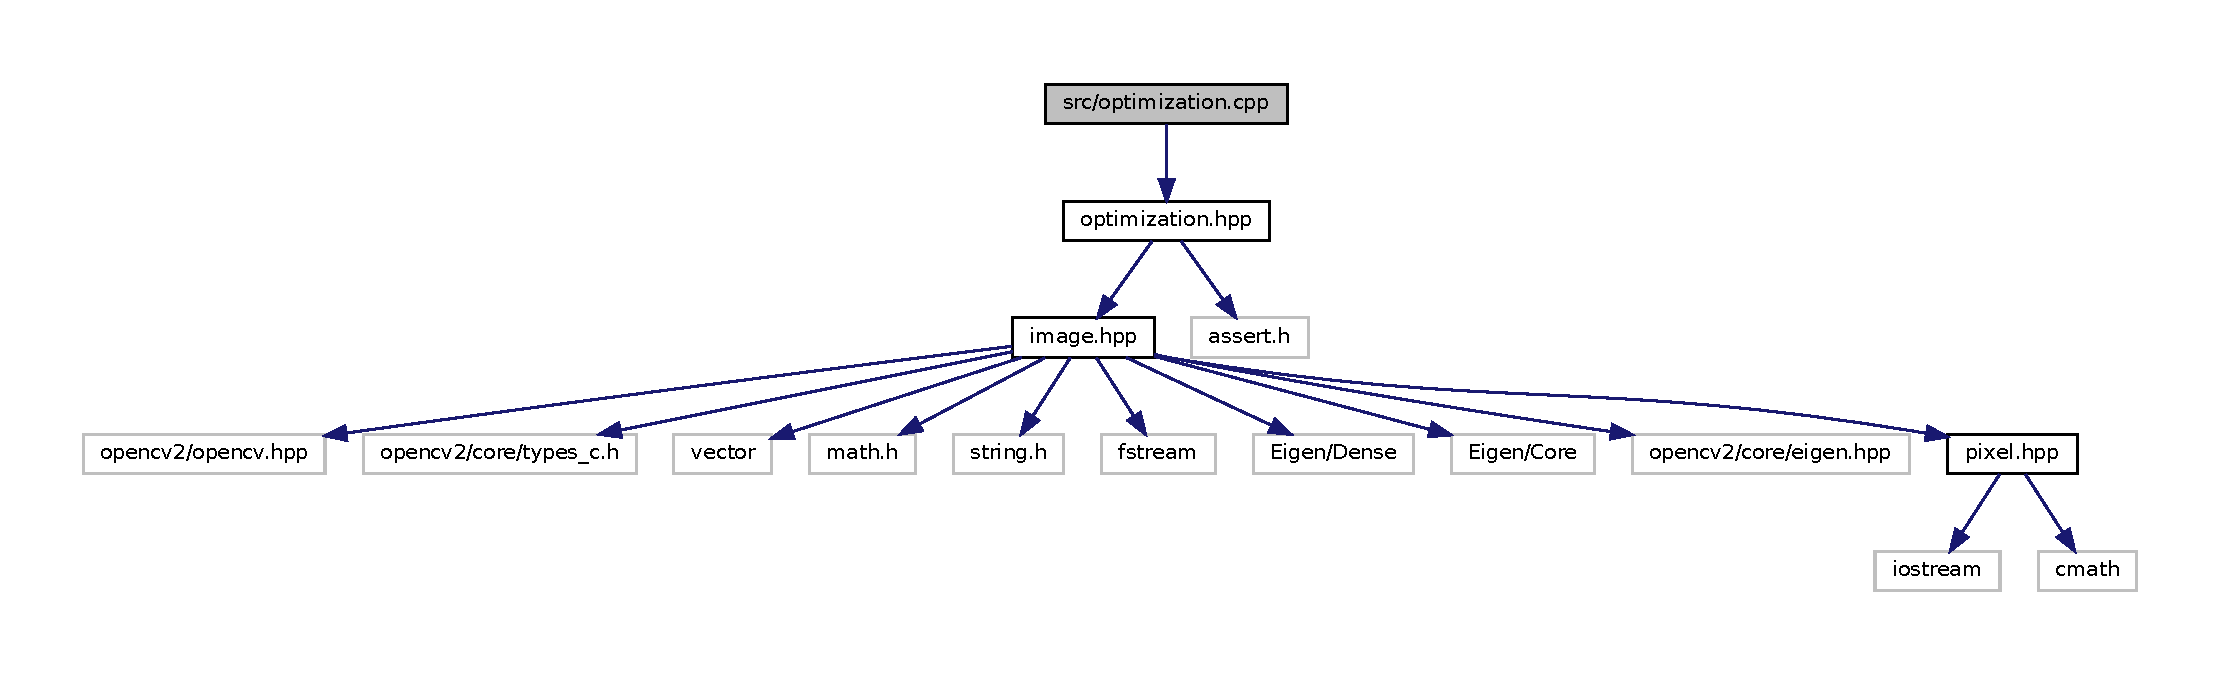
\includegraphics[width=350pt]{optimization_8cpp__incl}
\end{center}
\end{figure}
\subsection*{Functions}
\begin{DoxyCompactItemize}
\item 
int \hyperlink{optimization_8cpp_a3b6fe55e62e06469b89593c22dd51beb}{optimize} (std\+::vector$<$ float $>$ list\+\_\+l, bool squared)
\begin{DoxyCompactList}\small\item\em Find the index of the maximum or the minimum (correlation or squared error) of the values of loss function in the vector. \end{DoxyCompactList}\item 
bool \hyperlink{optimization_8cpp_a532ed4571db526e7215785ece8d31efe}{equal\+\_\+vector} (std\+::vector$<$ float $>$ \&v, std\+::vector$<$ float $>$ \&w)
\begin{DoxyCompactList}\small\item\em Function which return true if the two vectors are equals down to 0.\+001, false otherwise. \end{DoxyCompactList}\item 
void \hyperlink{optimization_8cpp_ae79ec3ddd049380a4bd091f05e7631fe}{copy\+\_\+tab3} (float tab1\mbox{[}3\mbox{]}, float tab2\mbox{[}3\mbox{]})
\end{DoxyCompactItemize}


\subsection{Detailed Description}
Set of optimization methods and function. 

Methods and function of optimization of the differents parameters of translation and rotation of the image. 

\subsection{Function Documentation}
\mbox{\Hypertarget{optimization_8cpp_ae79ec3ddd049380a4bd091f05e7631fe}\label{optimization_8cpp_ae79ec3ddd049380a4bd091f05e7631fe}} 
\index{optimization.\+cpp@{optimization.\+cpp}!copy\+\_\+tab3@{copy\+\_\+tab3}}
\index{copy\+\_\+tab3@{copy\+\_\+tab3}!optimization.\+cpp@{optimization.\+cpp}}
\subsubsection{\texorpdfstring{copy\+\_\+tab3()}{copy\_tab3()}}
{\footnotesize\ttfamily void copy\+\_\+tab3 (\begin{DoxyParamCaption}\item[{float}]{tab1\mbox{[}3\mbox{]},  }\item[{float}]{tab2\mbox{[}3\mbox{]} }\end{DoxyParamCaption})}

\mbox{\Hypertarget{optimization_8cpp_a532ed4571db526e7215785ece8d31efe}\label{optimization_8cpp_a532ed4571db526e7215785ece8d31efe}} 
\index{optimization.\+cpp@{optimization.\+cpp}!equal\+\_\+vector@{equal\+\_\+vector}}
\index{equal\+\_\+vector@{equal\+\_\+vector}!optimization.\+cpp@{optimization.\+cpp}}
\subsubsection{\texorpdfstring{equal\+\_\+vector()}{equal\_vector()}}
{\footnotesize\ttfamily bool equal\+\_\+vector (\begin{DoxyParamCaption}\item[{std\+::vector$<$ float $>$ \&}]{v,  }\item[{std\+::vector$<$ float $>$ \&}]{w }\end{DoxyParamCaption})}



Function which return true if the two vectors are equals down to 0.\+001, false otherwise. 


\begin{DoxyParams}{Parameters}
{\em two} & vectors of floats \\
\hline
\end{DoxyParams}
\mbox{\Hypertarget{optimization_8cpp_a3b6fe55e62e06469b89593c22dd51beb}\label{optimization_8cpp_a3b6fe55e62e06469b89593c22dd51beb}} 
\index{optimization.\+cpp@{optimization.\+cpp}!optimize@{optimize}}
\index{optimize@{optimize}!optimization.\+cpp@{optimization.\+cpp}}
\subsubsection{\texorpdfstring{optimize()}{optimize()}}
{\footnotesize\ttfamily int optimize (\begin{DoxyParamCaption}\item[{std\+::vector$<$ float $>$}]{list\+\_\+l,  }\item[{bool}]{squared }\end{DoxyParamCaption})}



Find the index of the maximum or the minimum (correlation or squared error) of the values of loss function in the vector. 


\begin{DoxyParams}{Parameters}
{\em a} & vector of the loss function values for a set of images, a boolean which is true if the loss function used is the squared error, false if it\textquotesingle{}s the correlation. \\
\hline
\end{DoxyParams}
\begin{DoxyReturn}{Returns}
the index of the optimized value in the vector 
\end{DoxyReturn}

\hypertarget{pixel_8cpp}{}\section{src/pixel.cpp File Reference}
\label{pixel_8cpp}\index{src/pixel.\+cpp@{src/pixel.\+cpp}}
{\ttfamily \#include \char`\"{}pixel.\+hpp\char`\"{}}\newline
Include dependency graph for pixel.\+cpp\+:
\nopagebreak
\begin{figure}[H]
\begin{center}
\leavevmode
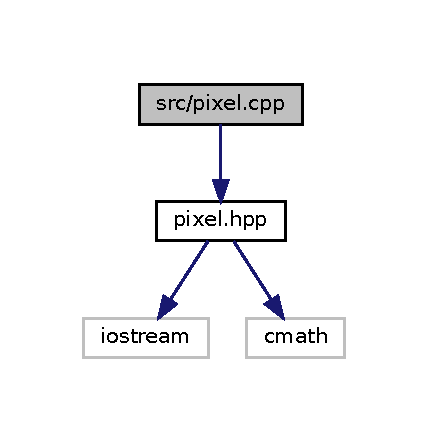
\includegraphics[width=206pt]{pixel_8cpp__incl}
\end{center}
\end{figure}

\hypertarget{pressure_8cpp}{}\section{src/pressure.cpp File Reference}
\label{pressure_8cpp}\index{src/pressure.\+cpp@{src/pressure.\+cpp}}


Set of methods and functions to simulate a variation of finger pressure during acquisition.  


{\ttfamily \#include \char`\"{}pressure.\+hpp\char`\"{}}\newline
Include dependency graph for pressure.\+cpp\+:
\nopagebreak
\begin{figure}[H]
\begin{center}
\leavevmode
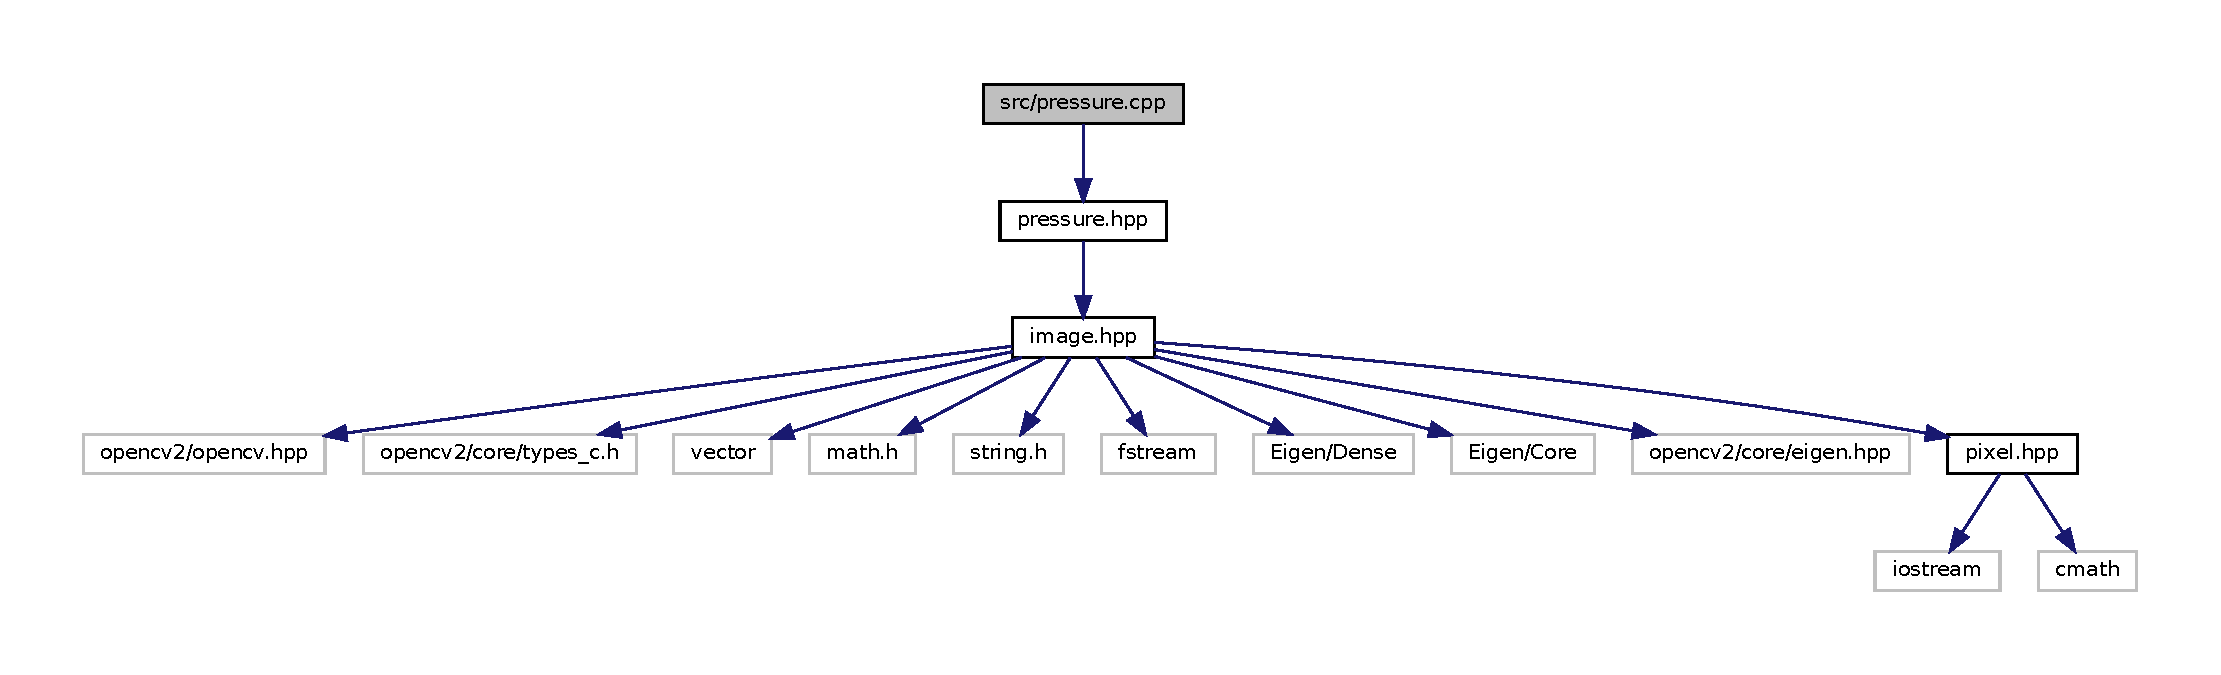
\includegraphics[width=350pt]{pressure_8cpp__incl}
\end{center}
\end{figure}
\subsection*{Macros}
\begin{DoxyCompactItemize}
\item 
\#define \hyperlink{pressure_8cpp_a17d00fb31c1fd9d49d75e28e3a2b987f}{attenuation\+\_\+power}~70
\begin{DoxyCompactList}\small\item\em Power of the exponential attenuation function which caracterizes the attenuation. \end{DoxyCompactList}\end{DoxyCompactItemize}
\subsection*{Functions}
\begin{DoxyCompactItemize}
\item 
float \hyperlink{pressure_8cpp_a44fb8b67c9a0fb92ac38e1c5d3cae7cd}{weight\+\_\+exp} (float coeff, int power, float r)
\begin{DoxyCompactList}\small\item\em Exponential attenuation function. \end{DoxyCompactList}\end{DoxyCompactItemize}


\subsection{Detailed Description}
Set of methods and functions to simulate a variation of finger pressure during acquisition. 



\subsection{Macro Definition Documentation}
\mbox{\Hypertarget{pressure_8cpp_a17d00fb31c1fd9d49d75e28e3a2b987f}\label{pressure_8cpp_a17d00fb31c1fd9d49d75e28e3a2b987f}} 
\index{pressure.\+cpp@{pressure.\+cpp}!attenuation\+\_\+power@{attenuation\+\_\+power}}
\index{attenuation\+\_\+power@{attenuation\+\_\+power}!pressure.\+cpp@{pressure.\+cpp}}
\subsubsection{\texorpdfstring{attenuation\+\_\+power}{attenuation\_power}}
{\footnotesize\ttfamily \#define attenuation\+\_\+power~70}



Power of the exponential attenuation function which caracterizes the attenuation. 



\subsection{Function Documentation}
\mbox{\Hypertarget{pressure_8cpp_a44fb8b67c9a0fb92ac38e1c5d3cae7cd}\label{pressure_8cpp_a44fb8b67c9a0fb92ac38e1c5d3cae7cd}} 
\index{pressure.\+cpp@{pressure.\+cpp}!weight\+\_\+exp@{weight\+\_\+exp}}
\index{weight\+\_\+exp@{weight\+\_\+exp}!pressure.\+cpp@{pressure.\+cpp}}
\subsubsection{\texorpdfstring{weight\+\_\+exp()}{weight\_exp()}}
{\footnotesize\ttfamily float weight\+\_\+exp (\begin{DoxyParamCaption}\item[{float}]{coeff,  }\item[{int}]{power,  }\item[{float}]{r }\end{DoxyParamCaption})}



Exponential attenuation function. 


\begin{DoxyParams}{Parameters}
{\em \hyperlink{class_image}{Image}} & \+: float \+: coefficient of attenuation, int \+: power, float \+: parameter. \\
\hline
\end{DoxyParams}

\hypertarget{rotation_8cpp}{}\section{src/rotation.cpp File Reference}
\label{rotation_8cpp}\index{src/rotation.\+cpp@{src/rotation.\+cpp}}
{\ttfamily \#include \char`\"{}image.\+hpp\char`\"{}}\newline
Include dependency graph for rotation.\+cpp\+:
\nopagebreak
\begin{figure}[H]
\begin{center}
\leavevmode
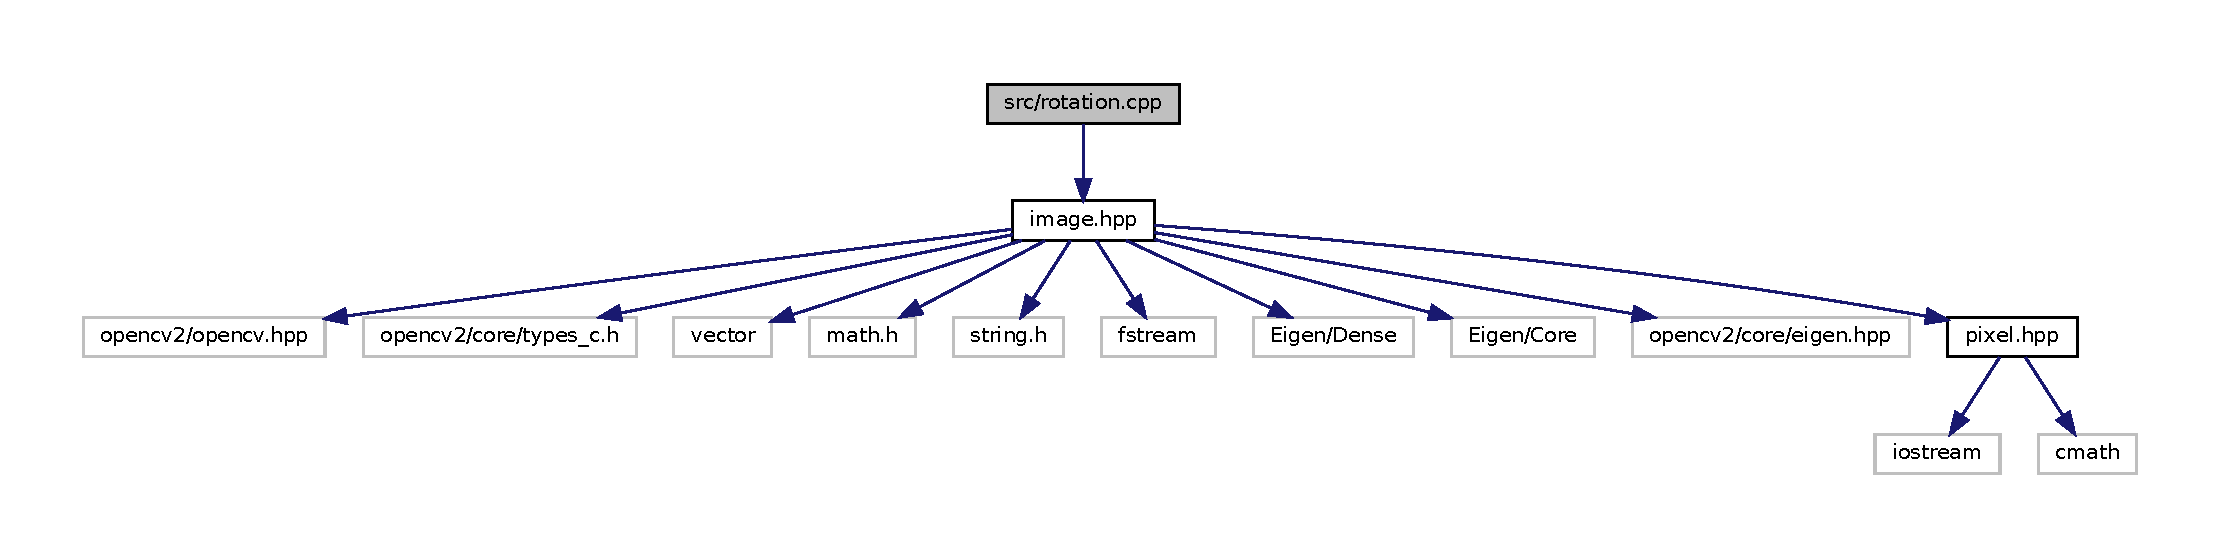
\includegraphics[width=350pt]{rotation_8cpp__incl}
\end{center}
\end{figure}

\hypertarget{translation_8cpp}{}\section{src/translation.cpp File Reference}
\label{translation_8cpp}\index{src/translation.\+cpp@{src/translation.\+cpp}}


Set of methods to translate the image along the x and y axis.  


{\ttfamily \#include \char`\"{}image.\+hpp\char`\"{}}\newline
Include dependency graph for translation.\+cpp\+:
\nopagebreak
\begin{figure}[H]
\begin{center}
\leavevmode
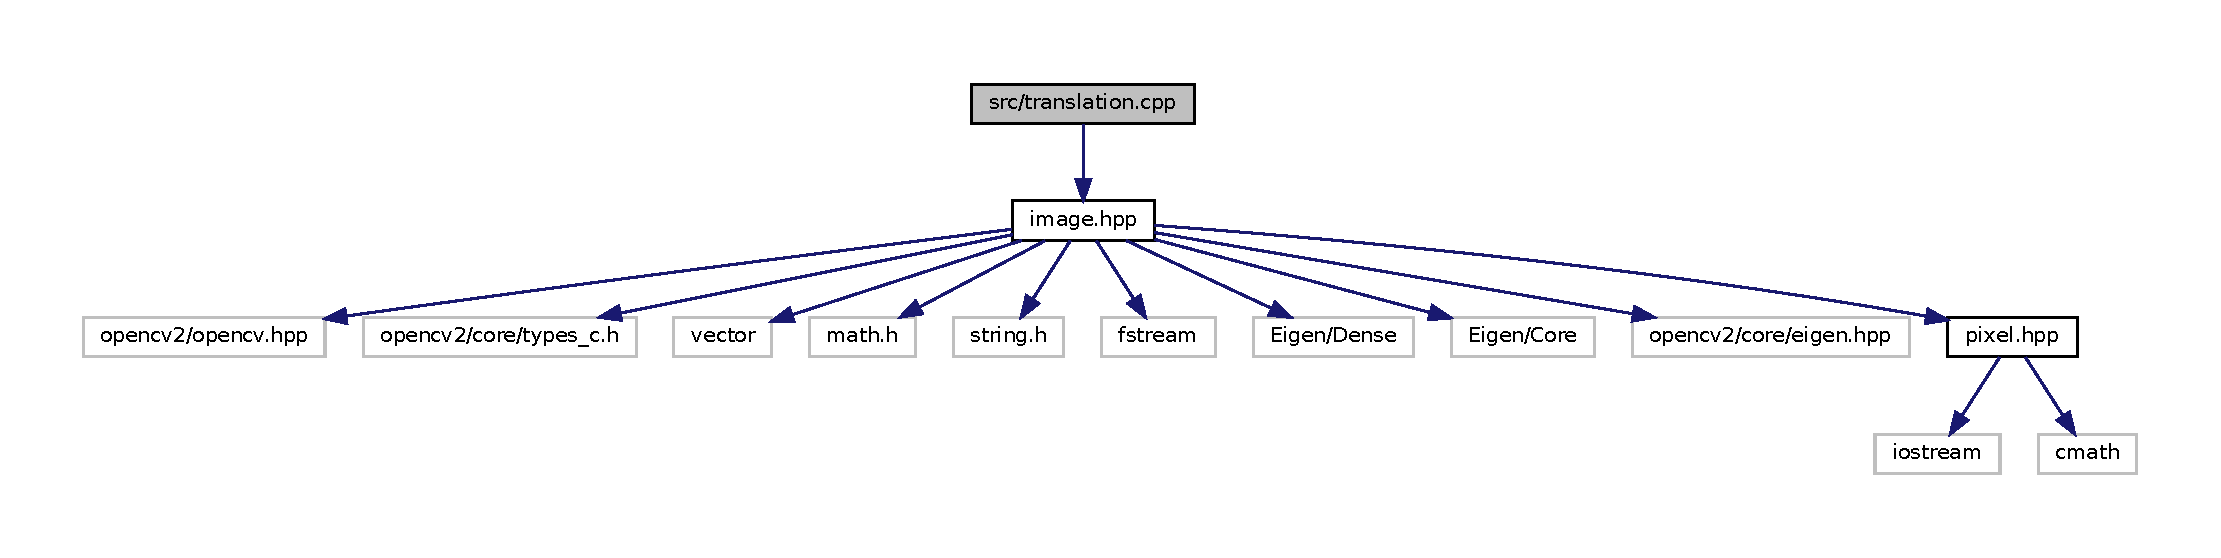
\includegraphics[width=350pt]{translation_8cpp__incl}
\end{center}
\end{figure}


\subsection{Detailed Description}
Set of methods to translate the image along the x and y axis. 


\hypertarget{warpping_8cpp}{}\section{src/warpping.cpp File Reference}
\label{warpping_8cpp}\index{src/warpping.\+cpp@{src/warpping.\+cpp}}
{\ttfamily \#include \char`\"{}image.\+hpp\char`\"{}}\newline
Include dependency graph for warpping.\+cpp\+:
\nopagebreak
\begin{figure}[H]
\begin{center}
\leavevmode
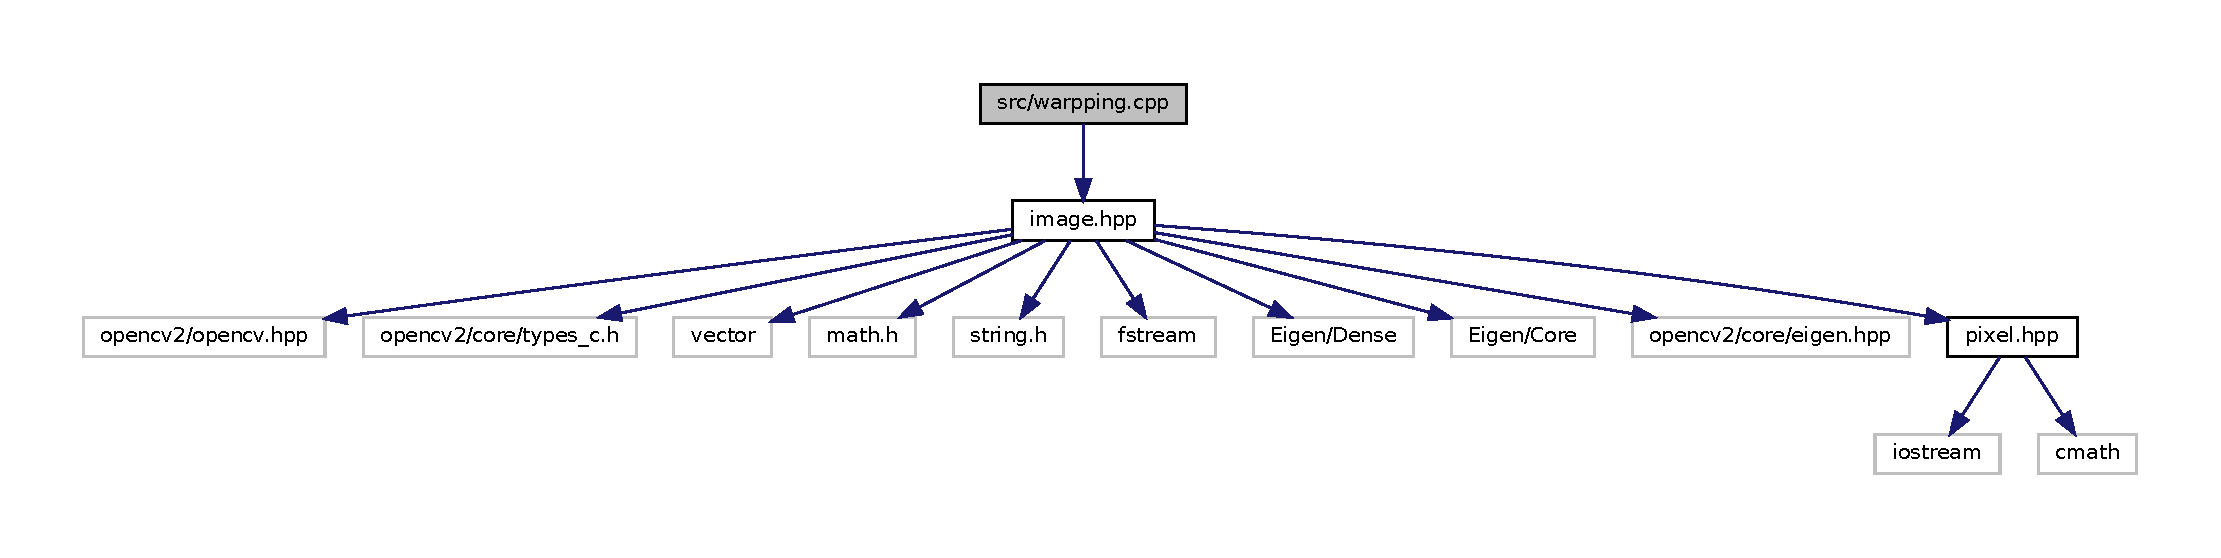
\includegraphics[width=350pt]{warpping_8cpp__incl}
\end{center}
\end{figure}

\hypertarget{test__optimization_8cxx}{}\section{tests/test\+\_\+optimization.cxx File Reference}
\label{test__optimization_8cxx}\index{tests/test\+\_\+optimization.\+cxx@{tests/test\+\_\+optimization.\+cxx}}
{\ttfamily \#include \char`\"{}image.\+hpp\char`\"{}}\newline
{\ttfamily \#include \char`\"{}optimization.\+hpp\char`\"{}}\newline
{\ttfamily \#include $<$gtest/gtest.\+h$>$}\newline
Include dependency graph for test\+\_\+optimization.\+cxx\+:
\nopagebreak
\begin{figure}[H]
\begin{center}
\leavevmode
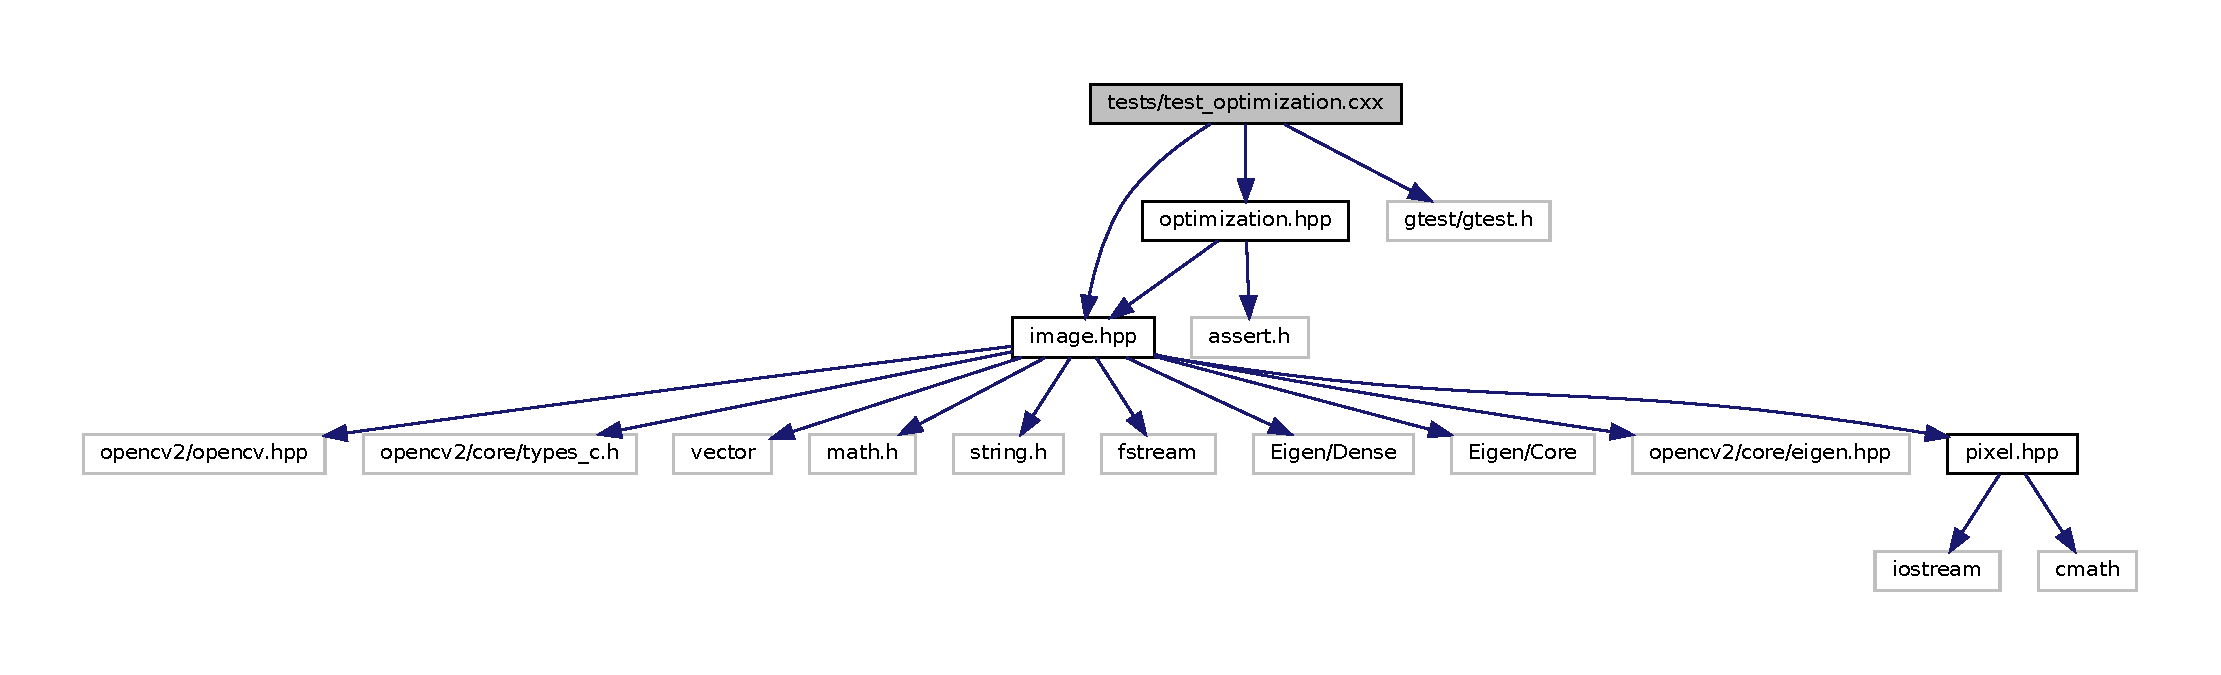
\includegraphics[width=350pt]{test__optimization_8cxx__incl}
\end{center}
\end{figure}
\subsection*{Functions}
\begin{DoxyCompactItemize}
\item 
\hyperlink{test__optimization_8cxx_a986e2df53bea239d52250bfaf61862de}{T\+E\+ST} (\hyperlink{optimization_8cpp_a3b6fe55e62e06469b89593c22dd51beb}{optimize}, max\+\_\+or\+\_\+min\+\_\+list)
\item 
\hyperlink{test__optimization_8cxx_ac311ad0bf8c88f073faa25ac9314ee84}{T\+E\+ST} (opti\+\_\+greedy\+\_\+x, px\+\_\+translation)
\item 
\hyperlink{test__optimization_8cxx_a7ed235a1ddd752bf4d8ca16402646f12}{T\+E\+ST} (opti\+\_\+greedy\+\_\+fast\+\_\+xy, px\+\_\+py\+\_\+translation)
\item 
\hyperlink{test__optimization_8cxx_adef8f3684769ff63c4197aa0e6576291}{T\+E\+ST} (coord\+\_\+descent, px\+\_\+py\+\_\+angle)
\item 
int \hyperlink{test__optimization_8cxx_a0ddf1224851353fc92bfbff6f499fa97}{main} (int argc, char $\ast$argv\mbox{[}$\,$\mbox{]})
\end{DoxyCompactItemize}


\subsection{Function Documentation}
\mbox{\Hypertarget{test__optimization_8cxx_a0ddf1224851353fc92bfbff6f499fa97}\label{test__optimization_8cxx_a0ddf1224851353fc92bfbff6f499fa97}} 
\index{test\+\_\+optimization.\+cxx@{test\+\_\+optimization.\+cxx}!main@{main}}
\index{main@{main}!test\+\_\+optimization.\+cxx@{test\+\_\+optimization.\+cxx}}
\subsubsection{\texorpdfstring{main()}{main()}}
{\footnotesize\ttfamily int main (\begin{DoxyParamCaption}\item[{int}]{argc,  }\item[{char $\ast$}]{argv\mbox{[}$\,$\mbox{]} }\end{DoxyParamCaption})}

\mbox{\Hypertarget{test__optimization_8cxx_a986e2df53bea239d52250bfaf61862de}\label{test__optimization_8cxx_a986e2df53bea239d52250bfaf61862de}} 
\index{test\+\_\+optimization.\+cxx@{test\+\_\+optimization.\+cxx}!T\+E\+ST@{T\+E\+ST}}
\index{T\+E\+ST@{T\+E\+ST}!test\+\_\+optimization.\+cxx@{test\+\_\+optimization.\+cxx}}
\subsubsection{\texorpdfstring{T\+E\+S\+T()}{TEST()}\hspace{0.1cm}{\footnotesize\ttfamily [1/4]}}
{\footnotesize\ttfamily T\+E\+ST (\begin{DoxyParamCaption}\item[{\hyperlink{optimization_8cpp_a3b6fe55e62e06469b89593c22dd51beb}{optimize}}]{,  }\item[{max\+\_\+or\+\_\+min\+\_\+list}]{ }\end{DoxyParamCaption})}

\mbox{\Hypertarget{test__optimization_8cxx_ac311ad0bf8c88f073faa25ac9314ee84}\label{test__optimization_8cxx_ac311ad0bf8c88f073faa25ac9314ee84}} 
\index{test\+\_\+optimization.\+cxx@{test\+\_\+optimization.\+cxx}!T\+E\+ST@{T\+E\+ST}}
\index{T\+E\+ST@{T\+E\+ST}!test\+\_\+optimization.\+cxx@{test\+\_\+optimization.\+cxx}}
\subsubsection{\texorpdfstring{T\+E\+S\+T()}{TEST()}\hspace{0.1cm}{\footnotesize\ttfamily [2/4]}}
{\footnotesize\ttfamily T\+E\+ST (\begin{DoxyParamCaption}\item[{opti\+\_\+greedy\+\_\+x}]{,  }\item[{px\+\_\+translation}]{ }\end{DoxyParamCaption})}

\mbox{\Hypertarget{test__optimization_8cxx_a7ed235a1ddd752bf4d8ca16402646f12}\label{test__optimization_8cxx_a7ed235a1ddd752bf4d8ca16402646f12}} 
\index{test\+\_\+optimization.\+cxx@{test\+\_\+optimization.\+cxx}!T\+E\+ST@{T\+E\+ST}}
\index{T\+E\+ST@{T\+E\+ST}!test\+\_\+optimization.\+cxx@{test\+\_\+optimization.\+cxx}}
\subsubsection{\texorpdfstring{T\+E\+S\+T()}{TEST()}\hspace{0.1cm}{\footnotesize\ttfamily [3/4]}}
{\footnotesize\ttfamily T\+E\+ST (\begin{DoxyParamCaption}\item[{opti\+\_\+greedy\+\_\+fast\+\_\+xy}]{,  }\item[{px\+\_\+py\+\_\+translation}]{ }\end{DoxyParamCaption})}

\mbox{\Hypertarget{test__optimization_8cxx_adef8f3684769ff63c4197aa0e6576291}\label{test__optimization_8cxx_adef8f3684769ff63c4197aa0e6576291}} 
\index{test\+\_\+optimization.\+cxx@{test\+\_\+optimization.\+cxx}!T\+E\+ST@{T\+E\+ST}}
\index{T\+E\+ST@{T\+E\+ST}!test\+\_\+optimization.\+cxx@{test\+\_\+optimization.\+cxx}}
\subsubsection{\texorpdfstring{T\+E\+S\+T()}{TEST()}\hspace{0.1cm}{\footnotesize\ttfamily [4/4]}}
{\footnotesize\ttfamily T\+E\+ST (\begin{DoxyParamCaption}\item[{coord\+\_\+descent}]{,  }\item[{px\+\_\+py\+\_\+angle}]{ }\end{DoxyParamCaption})}


\hypertarget{test__rotation_8cxx}{}\section{tests/test\+\_\+rotation.cxx File Reference}
\label{test__rotation_8cxx}\index{tests/test\+\_\+rotation.\+cxx@{tests/test\+\_\+rotation.\+cxx}}
{\ttfamily \#include \char`\"{}image.\+hpp\char`\"{}}\newline
{\ttfamily \#include \char`\"{}optimization.\+hpp\char`\"{}}\newline
{\ttfamily \#include $<$gtest/gtest.\+h$>$}\newline
Include dependency graph for test\+\_\+rotation.\+cxx\+:
\nopagebreak
\begin{figure}[H]
\begin{center}
\leavevmode
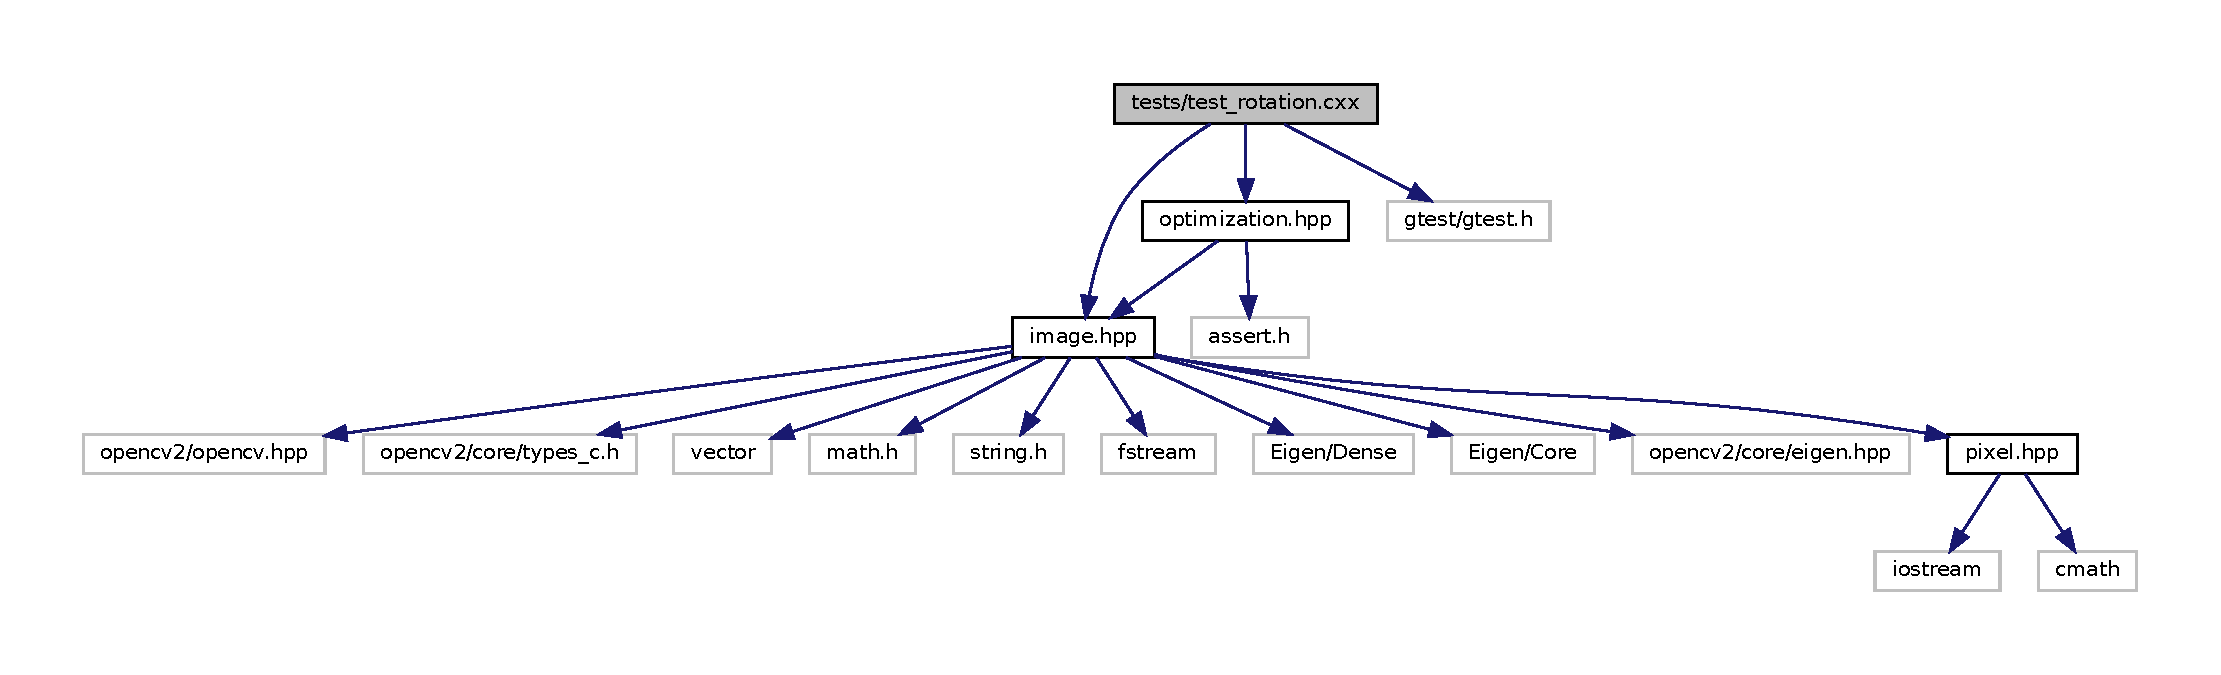
\includegraphics[width=350pt]{test__rotation_8cxx__incl}
\end{center}
\end{figure}
\subsection*{Functions}
\begin{DoxyCompactItemize}
\item 
\hyperlink{test__rotation_8cxx_ab3546aeee8ada090756fd9fd9dc33240}{T\+E\+ST} (rotate\+\_\+bilinear, erreur\+\_\+rotation)
\item 
int \hyperlink{test__rotation_8cxx_a0ddf1224851353fc92bfbff6f499fa97}{main} (int argc, char $\ast$argv\mbox{[}$\,$\mbox{]})
\end{DoxyCompactItemize}


\subsection{Function Documentation}
\mbox{\Hypertarget{test__rotation_8cxx_a0ddf1224851353fc92bfbff6f499fa97}\label{test__rotation_8cxx_a0ddf1224851353fc92bfbff6f499fa97}} 
\index{test\+\_\+rotation.\+cxx@{test\+\_\+rotation.\+cxx}!main@{main}}
\index{main@{main}!test\+\_\+rotation.\+cxx@{test\+\_\+rotation.\+cxx}}
\subsubsection{\texorpdfstring{main()}{main()}}
{\footnotesize\ttfamily int main (\begin{DoxyParamCaption}\item[{int}]{argc,  }\item[{char $\ast$}]{argv\mbox{[}$\,$\mbox{]} }\end{DoxyParamCaption})}

\mbox{\Hypertarget{test__rotation_8cxx_ab3546aeee8ada090756fd9fd9dc33240}\label{test__rotation_8cxx_ab3546aeee8ada090756fd9fd9dc33240}} 
\index{test\+\_\+rotation.\+cxx@{test\+\_\+rotation.\+cxx}!T\+E\+ST@{T\+E\+ST}}
\index{T\+E\+ST@{T\+E\+ST}!test\+\_\+rotation.\+cxx@{test\+\_\+rotation.\+cxx}}
\subsubsection{\texorpdfstring{T\+E\+S\+T()}{TEST()}}
{\footnotesize\ttfamily T\+E\+ST (\begin{DoxyParamCaption}\item[{rotate\+\_\+bilinear}]{,  }\item[{erreur\+\_\+rotation}]{ }\end{DoxyParamCaption})}


%--- End generated contents ---

% Index
\backmatter
\newpage
\phantomsection
\clearemptydoublepage
\addcontentsline{toc}{chapter}{Index}
\printindex

\end{document}
